\documentclass[11pt,reqno]{amsart}
\usepackage[margin=1.05in]{geometry}
\usepackage{amsmath,amssymb,amsthm,mathtools,booktabs,array,enumitem}
\usepackage[hyphens]{url}
\usepackage[colorlinks=true,linkcolor=blue,citecolor=blue,urlcolor=blue]{hyperref}
\usepackage[expansion=false]{microtype}
\usepackage{graphicx}
\usepackage{tikz}
\usetikzlibrary{calc}

\setlist{leftmargin=2em}
\emergencystretch=2em

\theoremstyle{plain}
\newtheorem{theorem}{Theorem}[section]
\newtheorem{proposition}[theorem]{Proposition}
\newtheorem{lemma}[theorem]{Lemma}
\newtheorem{corollary}[theorem]{Corollary}
\theoremstyle{definition}
\newtheorem{definition}[theorem]{Definition}
\newtheorem{remark}[theorem]{Remark}
\newtheorem{assumption}[theorem]{Assumption}

\newcommand{\R}{\mathbb R}
\newcommand{\hG}{h_\Gamma}
\newcommand{\hO}{h_\Omega}
\newcommand{\Gh}{\Gamma_h}
\newcommand{\Oh}{\Omega_h}
\newcommand{\Th}{\mathcal T_h}
\newcommand{\EG}{\mathcal E_h^\Gamma}
\newcommand{\Vh}{V_h}
\newcommand{\VR}{V_h^R}
\newcommand{\VO}{V_h^0}
\newcommand{\Pih}{\Pi_h}
\newcommand{\Zh}{Z_h}
\newcommand{\Wh}{W_h}
\newcommand{\Yh}{Y_h}
\newcommand{\gI}{g_I}
\newcommand{\dn}{\partial_n}
\newcommand{\dt}{\partial_\tau}
\newcommand{\ut}{\tilde u}
\newcommand{\pt}{\tilde p}
\newcommand{\ft}{\tilde f}
\newcommand{\psit}{\tilde\psi}
\newcommand{\pbar}{\bar p}
\newcommand{\pbG}{\bar p_{\Gamma}}
\newcommand{\ip}[2]{\langle #1,\, #2\rangle}
\newcommand{\tnorm}[1]{|\!|\!|#1|\!|\!|}
\newcommand{\norm}[1]{\lVert #1\rVert}
\newcommand{\GS}{\mathrm{GS}}
\newcommand{\CNS}{\mathrm{CNS}^\ast}
\newcommand{\eps}{\varepsilon_h}
\newcommand{\curl}{\operatorname{curl}}
\renewcommand{\div}{\operatorname{div}}
\newcommand{\Rc}{\mathcal R}
\newcommand{\Gc}{\mathcal G}
\newcommand{\cS}{\mathcal S}
\newcommand{\Lk}{\mathcal L}
\DeclareMathOperator{\diam}{diam}
\DeclareMathOperator{\dist}{dist}

\begin{document}

\title[Scott--Vogelius--Nitsche on polygonal boundaries]{Exactly divergence-free Stokes elements with Nitsche's method on a polygonally approximated boundary: the missing pressure traction, Scott's rate, and the zero-gradient lock}

\author{Jaideep Sai Padhi}
\address{Department of Computer Science, Purdue University, West Lafayette, IN 47907, USA}
\email{jpadhi@purdue.edu}
%% TBD: C. de S. Cavalcante may join as a co-author (per the joint AML letter); not added here.
\date{\today}
\subjclass[2020]{Primary 65N30; Secondary 65N12, 65N15, 76D07}
\keywords{Stokes equations, Scott--Vogelius elements, Nitsche's method, curved boundaries, polygonal approximation, divergence-free finite elements, penalty parameter}

\begin{abstract}
Scott--Vogelius elements compute velocities that are divergence-free pointwise, but on a curved no-slip wall this property clashes with the usual replacement of the wall by an inscribed polygon: the discrete velocity can be forced to have zero gradient at polygon vertices, and with strongly imposed no-slip the $H^1$ error can degrade to order $h^{1/2}$. Gjerde and Scott proposed to impose the wall condition weakly by Nitsche's method on the polygon, observed errors of order $h^{3/2}$, and Scott asked for a proof that the error behaves like $h_\Gamma^{3/2}+h_\Omega^k$ and, if it does not, why not. We answer the question in two dimensions.

For the method as printed, the estimate holds if and only if the pressure is constant along the wall. The printed Nitsche form omits the pressure part $-pn$ of the traction, so the penalty balances the wall pressure and the discrete velocity leaks through the wall with normal velocity $(h/\mu)(p-\bar p)$. We prove that the method nevertheless converges, at the sharp rate $h/\mu$ in the $H^1$ seminorm and $(h/\mu)^{1/2}$ in the mesh-dependent energy norm, identify the error to leading order with constant exactly $1$ in the slip and energy norms, and show that the $H^1$ constant is the energy of a Stokes flow driven by the leak. Restoring the traction with the wall mean of the discrete pressure removed gives a well-posed, exactly divergence-free method; the device is due to Frachon, Nilsson and Zahedi, and our contribution is its analysis. We prove that it attains $h_\Gamma^{3/2}+h_\Omega^k$ for general Stokes data and every fixed $k\ge4$, uniformly in the penalty for flux-corrected outer data, and that the term $h_\Gamma^{3/2}$ is sharp whenever the wall shear does not vanish identically and $h_\Gamma$ is small relative to the minimum angle of the wall triangles. We show that the Nitsche penalty must scale with the ratio of bulk to boundary mesh size, with sufficiency on every mesh and necessity certified in exact arithmetic on broad classes of meshes. Finally we explain the zero-gradient phenomenon itself: under the Guzm\'an--Scott angle condition strongly imposed no-slip already attains the same two-sided rate $h_\Gamma^{3/2}$, and the lock is caused by wall vertices lying in only two triangles, each of which costs $h_\Gamma|\partial_nu|$ in $H^1$. Computations with up to $256$ boundary chords confirm the rates and constants. Omitted proofs and further results are in an extended version.
\end{abstract}

\maketitle

\section{Introduction}\label{sec:intro}

\subsection{Exactly divergence-free elements}
Most mixed finite element methods for incompressible flow enforce the constraint $\div u=0$ only weakly: the discrete divergence is orthogonal to the discrete pressure space, but not zero. In 1985 Scott and Vogelius \cite{ScottVogelius1985} observed that for continuous piecewise-$P_k$ velocities and discontinuous piecewise-$P_{k-1}$ pressures the divergence maps the velocity space \emph{onto} the pressure space when $k\ge4$ and the mesh has no singular vertices. For such a pair the weak constraint is a strong one: the discrete velocity is divergence-free pointwise. The inf-sup constant of the pair was later made explicit in terms of the local geometry of the mesh by Guzm\'an and Scott \cite{GuzmanScott2019}, through an angle quantity $\Theta(z)$ at each vertex $z$ that measures how far the vertex is from being singular. Lower-degree pairs with the same property exist on split meshes, for instance on barycentric (Clough--Tocher) refinements \cite{ArnoldQin1992,GuzmanNeilan2018}; see Neilan's review \cite{Neilan2020}.

Pointwise incompressibility is more than a cosmetic property. It gives exact mass conservation, and, on meshes fitted to the domain with strongly imposed Dirichlet data, it makes the velocity error independent of the pressure. This \emph{pressure robustness} matters when pressure gradients are large relative to the viscosity, for example in nearly hydrostatic or rotating flows; the survey of John, Linke, Merdon, Neilan and Rebholz \cite{JohnEtAl2017} explains why the classical inf-sup stable pairs lack it and why divergence-free pairs have it.

\subsection{Curved walls and polygonal approximation}
Most flows of interest are bounded by curved walls. The simplest way to handle a curved boundary $\Gamma$ in a finite element code is to replace it by an inscribed polygon $\Gh$ whose vertices lie on $\Gamma$, and to impose the boundary condition on $\Gh$. For scalar second-order problems the consequences are classical. Berger, Scott and Strang \cite{BergerScottStrang1972} and Scott \cite{Scott1975} showed that transferring a homogeneous Dirichlet condition from $\Gamma$ to $\Gh$ costs an $H^1$ error of order $\hG^{3/2}$, where $\hG$ is the length of the chords: the solution is of size $\hG^2$ on the chords and oscillates on the scale $\hG$, so its $H^{1/2}(\Gh)$ norm is of order $\hG^{3/2}$. Higher order requires either a better geometry or a correction of the boundary data. The first route is the isoparametric approach, in which the boundary elements are curved by a polynomial map \cite{Ciarlet1978book}; the second goes back to Bramble, Dupont and Thom\'ee \cite{BrambleDupontThomee1972}, who corrected the boundary condition on the polygon by a Taylor expansion in the normal direction. Both ideas are alive today: boundary-value correction has been combined with Nitsche's method for cut elements \cite{BurmanHansboLarson2018,BurmanHansboLarson2019Stokes} and for polygonal approximations \cite{DupontGuzmanScott2025}, and the shifted boundary method \cite{MainScovazzi2018} is a related approach.

For exactly divergence-free elements the polygonal approximation has an additional, less obvious cost. A field that is smooth at a polygon vertex and vanishes on both adjacent edges has zero gradient there, since its gradient annihilates two independent directions. Continuous piecewise polynomials can escape this constraint, because their gradients may jump across the interior edges at the vertex; for \emph{divergence-free} piecewise polynomials, however, the jumps are themselves constrained, and such fields inherit gradient constraints at the vertices of a polygonal wall \cite{ScottPrize,GjerdeScott2024}. On the true curved wall, however, the gradient of the velocity is $\dn u\otimes n$, which is not zero where the wall shear stress is not zero. If no-slip is imposed strongly on an inscribed polygon, the computed gradient can therefore be wrong by $O(1)$ at the polygon vertices. Scott and Gjerde--Scott report that the $H^1$ error of Scott--Vogelius elements then decays only like $h^{1/2}$ \cite{ScottPrize,GjerdeScott2024}, compared with $h^{3/2}$ for scalar problems. We call this the \emph{zero-gradient lock}. The standard cure is to fit the geometry, with isoparametric or Piola-mapped Scott--Vogelius elements \cite{NeilanOtus2021,DurstNeilan2024}; these attain the optimal order $h^k$, at the price of curved elements.

\subsection{Nitsche's method and the prize question}
In 1971 Nitsche \cite{Nitsche1971} proposed to impose Dirichlet conditions weakly, by adding to the variational form a consistency term (the normal flux of the solution tested against the test function), its symmetric counterpart, and a penalty term $(\mu/h)\ip{u}{v}$. Unlike a pure penalty method \cite{Babuska1973}, whose penalty must grow as the mesh is refined because the method is inconsistent, Nitsche's method is consistent, so the penalty only has to be large enough for coercivity. Stenberg \cite{Stenberg1995} later showed that Nitsche's method can be read as a stabilised Lagrange multiplier method, which explains both its consistency and the form of its penalty; the multiplier is the boundary flux of the solution. For the Stokes equations the consistency term is the full traction $\sigma(u,p)n=(\nabla u)n-pn$ (or its symmetric-gradient version), and therefore contains the pressure term $\ip{p}{v\cdot n}$ \cite{FreundStenberg1995,Stenberg1995,Becker2002,BurmanHansbo2014}; Burman, Hansbo and Larson note that this term is essential for consistency \cite{BurmanHansboLarson2019Stokes}.

Gjerde and Scott \cite{GjerdeScott2024} combined these ideas: they keep the inscribed polygon, use Scott--Vogelius elements with $k=4$, and impose no-slip on the polygon by Nitsche's method, with penalty $\mu/h$ and \emph{no pressure term}. They report errors orders of magnitude below those of strong imposition. Scott observed $H^1$ errors of order $h^{3/2}$ for this Scott--Vogelius--Nitsche method on a benchmark with constant pressure, and posed the question as a prize problem, listed as PPL~115 in the Prize Problem Ledger \cite{ScottPrize}. The prize asks for ``a published proof that Scott--Vogelius--Nitsche converges'', which ``should include a computational study of the influence of the Nitsche penalty parameter''. It states the expected error
\[
\norm{u-u_h}_{H^1}\;\lesssim\;\hG^{3/2}+\hO^k,
\]
where $\hG$ is the boundary mesh size and $\hO$ the bulk mesh size, and it adds: \emph{``If this does not hold, why not?''} This paper answers the question, for general Stokes data, in two dimensions.

\subsection{What goes wrong, and why the method still converges}
The key observation is simple. Because the Gjerde--Scott form has no pressure term on the wall, the discrete momentum equation does not see the wall pressure through a traction. Testing the exact solution in the discrete equations leaves the residual $-\ip{p-\pbar}{v\cdot n}$ on the polygon, for any constant $\pbar$. Something must balance it, and the only candidate is the penalty. To leading order the discrete velocity therefore satisfies the \emph{leak law}
\[
\frac\mu h\,u_h\cdot n\;\approx\;p-\pbar\qquad\text{on }\Gh ,
\]
where $\pbar$ is the mean of $p$ over the wall: the fluid leaks through the wall, outward where the pressure is above its mean and inward where it is below. The leak is of size $h/\mu$, so it vanishes as the mesh is refined. This is the classical consistency error of a boundary penalty method \cite{Babuska1973}, acting only on the pressure and with the vanishing parameter $h/\mu$, and it is the reason why the printed method converges at all.

How fast does it converge? The leak is a normal velocity of size $h/\mu$ on the wall, so a naive trace argument would lift it to an $H^1$ error of order $(h/\mu)\hG^{-1/2}$, that is, rate $\frac12$. The true $H^1$ rate is $1$. The reason is incompressibility: for a divergence-free polynomial field on a boundary triangle, the normal derivative of the normal component equals minus the tangential derivative of the tangential component, so the purely \emph{normal} load produced by the missing traction acts like a tangential derivative and can be integrated by parts along the wall. In the mesh-dependent energy norm, which contains $(\mu/h)^{1/2}\norm{\cdot}_{L^2(\Gh)}$, the leak is seen directly and the rate is exactly $\frac12$. In short: the printed method converges, but not at Scott's rate, unless the pressure is constant along the wall. This explains why Scott's constant-pressure benchmark shows the rate $\frac32$, and it is the answer to ``why not'' for the method as printed.

\subsection{The repair}
The obvious repair is to add the missing term $\ip{p_h}{v\cdot n}$ to the momentum equation. With exactly divergence-free elements this does not work as it stands: the square linear system acquires the kernel vector $(u,p)=(0,1)$, because a constant pressure now drops out of both equations. The standard fix, restricting the pressure to mean-zero functions, destroys pointwise incompressibility: the discrete divergence becomes a nonzero constant. The repair we analyse adds the traction with the \emph{wall mean of the discrete pressure removed}, $\ip{p_h-\pbG(p_h)}{v\cdot n}$, to the momentum equation only. The continuity equation is untouched, so the velocity stays exactly divergence-free, and the constant mode is fixed automatically. We call this method $\CNS$ (consistent Nitsche, with the star marking the mean-free correction). The device is not new: Frachon, Nilsson and Zahedi \cite{FrachonNilssonZahedi2024} introduced the zero-net-flux formulation for divergence-free cut elements, and the velocity of $\CNS$ coincides with the velocity of their formulation transcribed to our setting. What is new is the analysis on an inscribed polygon.

\subsection{Main results}
We state the results informally here; precise statements are in Sections~\ref{sec:printed}--\ref{sec:strong}. We write $h=\hO$ for the bulk mesh size (the $h$ in Scott's penalty $\mu/h$), $\hG$ for the longest chord, $\gamma=\mu\hG/h$ for the effective boundary penalty, and $G=\norm{p-\pbar}_{L^2(\Gamma)}$ for the variation of the pressure along the wall. The solution is assumed smooth, the mesh shape regular, and every polygon vertex is assumed to lie in at least three triangles (this is the Guzm\'an--Scott angle condition at the wall; Section~\ref{sec:setting}).
\begin{enumerate}[label=(\arabic*)]
\item \emph{The printed method converges, but at rate $1$ when the wall pressure varies} (Section~\ref{sec:printed}). Its $H^1$ error is at most $C_p\,h/\mu+C(\hG^{3/2}+\hO^k)$, and at least $c\,(h/\mu)G$; in the energy norm it is $\asymp(h/\mu)^{1/2}G$ plus Scott's terms. To leading order the error is an explicit field whose trace is $-(h/\mu)(p-\pbar)n$; its slip and energy norms, normalised by $(h/\mu)G$ and $(h/\mu)^{1/2}G$, tend to $1$. The normalised $H^1$ error tends to the energy of the Stokes flow that has the leak as Dirichlet data. This constant depends on the whole domain, not only on the wall.
\item \emph{The mean-free correction attains Scott's rate, and the rate is sharp} (Section~\ref{sec:corrected}). $\CNS$ is well posed for $\gamma$ above a threshold, its velocity is divergence-free pointwise, and $\norm{u-u_h}_{H^1}\le C(\hG^{3/2}+\hO^k)$ for general Stokes data and every fixed $k\ge4$. With a zero-flux correction of the outer boundary data the bound is uniform in the penalty and needs no relation between $\hG$ and $\hO$. If the wall shear does not vanish identically and $\hG\le2\sin(\theta_{\min}/4)$, with $\theta_{\min}$ the minimum angle of the triangles at the wall, the $H^1$ error is also bounded below by $c\,\hG^{3/2}$, so the term $\hG^{3/2}$ cannot be improved.
\item \emph{The penalty must scale with the mesh ratio} (Section~\ref{sec:penalty}). With Scott's normalisation $\mu/h$, the penalty must grow like $\rho=h/\min_e|e|$. Sufficiency holds on every mesh. Necessity is certified in exact rational arithmetic on every mesh whose shortest chord carries a triangle with apex angle at least $35^\circ$ and base angles at least $5^\circ$, and is proved on every shape-regular mesh with explicit but very small constants. A necessity statement based on a single wall star is false in general (the exact counterexamples have small angles).
\item \emph{The zero-gradient lock is a property of the wall mesh} (Section~\ref{sec:strong}). Under the same angle condition, strongly imposed no-slip on the polygon already has $H^1$ error $\asymp\hG^{3/2}+h^k$, two-sided. The lock is caused by polygon vertices lying in only two triangles, which the angle condition excludes: each such vertex costs $\hG|\dn u(z)|$ in $H^1$, one lock gives rate $1$, and a positive fraction of locks gives rate $\frac12$. With three or more triangles the same loss appears continuously as one triangle at the vertex degenerates. The advantages of Nitsche imposition on an inscribed polygon are therefore robustness to such meshes and a smaller constant, not a better rate.
\end{enumerate}
Table~\ref{tab:summary} summarises the rates.

\begin{table}[htb]
\centering\small
\caption{Rates for $k\ge4$ on meshes satisfying the angle condition (M0)--(M2) of Section~\ref{sec:setting}, fixed penalty $\gamma$, smooth solution, $h\asymp\hG$. ``$G>0$'' means the pressure is not constant on the wall; ``$W\not\equiv0$'' means the wall shear does not vanish identically.}\label{tab:summary}
\setlength{\tabcolsep}{3pt}
\begin{tabular}{>{\raggedright\arraybackslash}p{0.29\textwidth}>{\raggedright\arraybackslash}p{0.33\textwidth}>{\raggedright\arraybackslash}p{0.15\textwidth}>{\raggedright\arraybackslash}p{0.14\textwidth}}
\toprule
method & $H^1$ error & energy error & where\\
\midrule
printed ($\GS$), $G=0$ & $\asymp\hG^{3/2}$ (if $W\not\equiv0$) & $\lesssim\hG^{3/2}$ & Thms.~\ref{thm:A}, \ref{thm:lb}\\
printed ($\GS$), $G>0$ & $\asymp h/\mu$ & $\asymp(h/\mu)^{1/2}$ & Thms.~\ref{thm:A}--\ref{thm:B}\\
printed, growing penalty $\mu\gtrsim h\hG^{-3/2}$ & $\asymp\hG^{3/2}$ & rate $\le1$ for any scaling & Cor.~\ref{cor:rescue}, Sec.~\ref{sec:growing}\\
corrected ($\CNS$), any $G$ & $\asymp\hG^{3/2}$ (if $W\not\equiv0$) & $\lesssim\hG^{3/2}$ & Thms.~\ref{thm:D}, \ref{thm:lb}\\
strong no-slip, $\ge3$ triangles at every wall vertex & $\asymp\hG^{3/2}$ & -- & Thm.~\ref{thm:st:two}\\
strong no-slip, locked wall vertices $\Lk$ & $\asymp\hG^{3/2}+\hG\bigl(\sum_{\Lk}|\dn u(z)|^2\bigr)^{1/2}$ & -- & Thm.~\ref{thm:st:locks}\\
\bottomrule
\end{tabular}
\end{table}

Beyond these four results, the extended version \cite{PadhiExt} of this paper, of which the present article is a condensed account, contains a theory of the pressure and of drag and lift, $L^2$ estimates, Clough--Tocher refinements with $k\ge2$, general curved domains, steady Navier--Stokes flow, nearly singular wall stars, and pressure robustness. We state these results without proof in Section~\ref{sec:further}. The three-dimensional analysis is the subject of a companion paper \cite{PadhiThreeD}.

\subsection{How to read this paper}
Section~\ref{sec:related} compares our results with the recent literature and lists precisely what is new. Section~\ref{sec:setting} fixes the setting and collects the geometric and discrete tools. Section~\ref{sec:printed} analyses the printed method, Section~\ref{sec:corrected} the corrected method, Section~\ref{sec:penalty} the penalty threshold and Section~\ref{sec:strong} strong imposition. Section~\ref{sec:further} surveys further results, Section~\ref{sec:numerics} reports computations, and Section~\ref{sec:conclusions} concludes with open problems. Proofs that are routine, or that rely on long computer-assisted certificates, are sketched and referred to \cite{PadhiExt}; the code and all raw data are publicly available \cite{ZeroGradRepo}.

\section{Related work and novelty}\label{sec:related}

The problem sits at the meeting point of three lines of work: exactly divergence-free elements on curved domains, weak imposition of boundary conditions for Stokes flow, and the stability theory of Scott--Vogelius elements near singular and nearly singular vertices. We discuss each and then state what is new.

\subsection{The prize problem and the constant-pressure case}
The question we answer was posed by Scott \cite{ScottPrize}, on the basis of the computations of Gjerde and Scott \cite{GjerdeScott2024}. Cavalcante \cite{Cavalcante} has analysed the constant-pressure (zero-pressure-gradient) benchmark of the prize: the abstract of that preprint states the bound $\norm{u-u_h}_{H^1}\le C(\hO^k+\hG^{3/2})$ for this benchmark with quartic velocities on an inscribed polygon, and it reports a coercivity transition of the penalty near $\mu\approx60.338$ for its test mesh; our code gives $\mu^\ast=60.343$ at the same resolution ($N=20$ chords). In our notation that is the case $G=0$ of the printed method, which we recover in Theorem~\ref{thm:A}; our proofs do not use \cite{Cavalcante}. The present paper treats general Stokes data. The difference is essential: once the wall pressure varies, the printed method no longer has Scott's rate (Theorems~\ref{thm:A}--\ref{thm:B}), and a corrected method is needed. The analysis of the constant-pressure case and ours are thus complementary answers to the two halves of Scott's question: the ``if'' (the estimate holds when the pressure is constant on the wall) and the ``why not'' (it fails otherwise, for an identifiable reason).

\subsection{Divergence-free elements on curved domains}
Neilan and Otus \cite{NeilanOtus2021} constructed Scott--Vogelius elements on curved two-dimensional domains, with boundary elements mapped to fit the geometry, and proved convergence estimates; they also showed how to recover pressure robustness by reconstructing the load with commuting interpolants \cite[Theorem~6.1]{NeilanOtus2021}. Durst and Neilan \cite{DurstNeilan2024} extended the approach to general degree on smooth planar domains. In three dimensions, Chen and Liu \cite{ChenLiu2026} obtain pressure-robust, optimal-order $h^k$ estimates with isoparametric Piola-mapped elements on curved domains. Methods that fit the boundary can reach rates above $\hG^{3/2}$ (Chen and Liu attain $h^k$); the inscribed-polygon Nitsche route analysed here is the low-cost, straight-sided alternative, whose best possible rate is $\hG^{3/2}+h^k$ (Theorem~\ref{thm:lb}). We therefore do not regard it as a competitor on rate, but as the analysis of a method that is easy to implement in any code that already has Scott--Vogelius elements.

The work closest to ours is that of Liu, Neilan and Otus \cite{LiuNeilanOtus2023}. They use Scott--Vogelius elements on Clough--Tocher splits of a mesh lying inside a curved domain, impose the tangential condition by a Nitsche-type form with a Taylor boundary correction, and enforce the normal component by a separate mean-free boundary multiplier which, as they note, approximates the wall pressure up to a constant. Together with a zero-flux constraint on the velocity space the method is exactly divergence-free and converges at the optimal order $h^k$; without the constraint, they remark, it is ill posed \cite[Remark~3.2]{LiuNeilanOtus2023}. Our Proposition~\ref{prop:singular} is the analogue of this remark for the square Scott--Vogelius system. Our subject is different: the method as Gjerde and Scott printed it, and its minimal repair, with no extra unknowns, no boundary correction and the pressure itself on the wall.

For cut (unfitted) meshes, Liu, Neilan and Olshanskii \cite{LiuNeilanOlshanskii2023} place the boundary pressure term in both the momentum and the continuity equation; the discrete divergence then vanishes only away from an $O(h)$ strip at the boundary. Frachon, Nilsson and Zahedi \cite{FrachonNilssonZahedi2024} place it in the momentum equation only, so as not to perturb the divergence condition, and show that fixing the pressure mean by a Lagrange multiplier makes the discrete divergence equal to that multiplier \cite[(5.7)--(5.9)]{FrachonNilssonZahedi2024}. They avoid this by testing the momentum equation only with velocities of zero net boundary flux. Our $\CNS$ is this device in square form (Remark~\ref{rem:fnz}); we claim no novelty for it. Burman, Hansbo and Larson give related multiplier formulations for divergence-free cut elements \cite{BurmanHansboLarson2024}. Exactly divergence-free methods also require discrete Dirichlet data with zero net flux, as Eickmann, Scott and Tscherpel point out for polygonal domains \cite{EickmannScottTscherpel2025}; our flux-corrected outer data (Definition~\ref{def:flux}) are a simple instance.

\subsection{Nitsche's method for Stokes flow}
Weak imposition of Dirichlet data in Nitsche's sense was developed further by Freund and Stenberg \cite{FreundStenberg1995} and Stenberg \cite{Stenberg1995}; for Stokes flow the consistent form uses the full traction and contains the pressure term \cite{FreundStenberg1995,Stenberg1995,Becker2002,BurmanHansbo2014}. Penalty-free variants \cite{Burman2012,BoiveauBurman2016} and Robin-type generalisations \cite{JuntunenStenberg2009} exist. That the pressure term is needed for consistency is known \cite{BurmanHansboLarson2019Stokes}, and that the Nitsche penalty must scale with the local boundary mesh size follows from the trace-inverse inequality \cite{Stenberg1995,JuntunenStenberg2009}. What has not been done, to our knowledge, is an analysis of a Nitsche--Stokes form \emph{without} the pressure term: whether it converges, at what rate, and what its error looks like. The mechanism, a consistency error of penalty type acting only on the pressure, is that of Babu\v{s}ka's penalty method \cite{Babuska1973}.

On the geometric side, the polygonal approximation of curved boundaries for scalar problems is classical \cite{BergerScottStrang1972,Scott1975}, and higher-order boundary corrections on polygons are due to Bramble, Dupont and Thom\'ee \cite{BrambleDupontThomee1972} and, more recently, Dupont, Guzm\'an and Scott \cite{DupontGuzmanScott2025} (for the Poisson problem). Bernardi, Costabel, Dauge and Girault \cite{BCDG2016} show that the continuous inf-sup constant of an inscribed polygonal approximation converges to that of the curved domain; we use a simple gluing argument for the same purpose. None of the cut-element or boundary-correction works above uses exactly divergence-free spaces on an inscribed polygon.

\subsection{Singular and nearly singular vertices}
The stability of Scott--Vogelius elements degenerates near singular vertices, and the Guzm\'an--Scott quantity $\Theta(z)$ \cite{GuzmanScott2019} measures this. Gr\"a\ss le, Bohne and Sauter \cite{GrassleBohneSauter2024} introduced pressure constraints (the ``pressure-wired'' element) that restore a shape-robust inf-sup constant at nearly singular vertices, and spurious pressures with robust velocities, together with postprocessing filters, were studied by Park \cite{Park2020} and by Bohne, Gr\"a\ss le and Sauter \cite{BohneGrassleSauter2025}. Our constrained inf-sup result for strong imposition (Theorem~\ref{thm:st:locks}(a)) is essentially the wall-vertex case of theirs, and our pressure filter is in the same spirit. Kean, Neilan and Schneier \cite{KeanNeilanSchneier2022} analyse Scott--Vogelius elements on anisotropic meshes obtained by barycentric and incenter refinement. What is different in our setting is that the loss at a locked wall vertex is an \emph{approximation} loss, caused by the zero trace on the polygon, and not a stability loss; the velocity error can therefore be characterised two-sidedly.

The zero-gradient lock at a wall vertex with two triangles, and the statement that no constraint arises with more than two triangles, are due to Scott \cite[Theorem~1]{ScottPrize}; Gjerde and Scott treat the two-triangle case in \cite[\S3.4, App.~B]{GjerdeScott2024}.

\subsection{Broader context}
Several further strands of the literature enter the analysis or its extensions. The divergence-free pairs used in three dimensions, relevant to the companion paper \cite{PadhiThreeD}, are stable on Alfeld (barycentric) splits \cite{Zhang2005,GuzmanNeilan2018}, on Worsey--Farin splits \cite{GuzmanLischkeNeilan2022}, and on Freudenthal meshes for large degree \cite{Zhang2011}; smooth discrete de Rham complexes \cite{Neilan2015,FuGuzmanNeilan2020} provide the corresponding smooth stream-function spaces, and Farrell, Mitchell and Scott \cite{FarrellMitchellScott2024} survey what is known and conjectured. A local Fortin projection for Scott--Vogelius elements on general meshes has recently been constructed by Eickmann, Guzm\'an, Neilan, Scott and Tscherpel \cite{EickmannGNST2026}. Our $L^2$ estimates on graded meshes use local energy estimates in the spirit of Arnold and Liu \cite{ArnoldLiu1995} and of Demlow, Guzm\'an and Schatz \cite{DemlowGuzmanSchatz2011}, and the regularity result of Kellogg and Osborn \cite{KelloggOsborn1976} on convex polygons. The Navier--Stokes extension follows the framework of nonsingular solution branches of Brezzi, Rappaz and Raviart \cite{BRR1980,GiraultRaviart}, with a duality argument of Schatz type \cite{Schatz1974} for explicit thresholds. Sharp trace-inverse constants for polynomials \cite{WarburtonHesthaven2003} enter the analysis of the pressure in the first row of boundary triangles. For nearly singular wall stars we use anisotropic interpolation \cite{BabuskaAziz1976,Apel1999} and right inverses of the divergence on John domains \cite{AcostaDuranMuschietti2006}.

\subsection{What is known and what is new}
\emph{Known, and used or recovered here.}
\begin{itemize}
\item The pressure term is necessary for consistency of Nitsche's method for Stokes flow \cite{BurmanHansboLarson2019Stokes}; penalty consistency errors of the leak type are classical \cite{Babuska1973}.
\item The mean-free (zero-net-flux) placement of the pressure term that keeps the discrete velocity divergence-free \cite{FrachonNilssonZahedi2024}; the need for a flux constraint or correction \cite{LiuNeilanOtus2023,EickmannScottTscherpel2025}.
\item Sufficiency of a penalty proportional to the ratio of bulk to boundary mesh size (the trace-inverse inequality \cite{Stenberg1995,JuntunenStenberg2009}).
\item The two-triangle lock \cite{ScottPrize,GjerdeScott2024}; constrained and filtered pressures at nearly singular vertices \cite{GrassleBohneSauter2024,Park2020,BohneGrassleSauter2025}.
\item The $H^1$ bound $\hO^k+\hG^{3/2}$ for the constant-pressure benchmark with quartic velocities \cite{Cavalcante}.
\end{itemize}
\emph{New in this paper}, as far as we know.
\begin{itemize}
\item A two-sided analysis of the printed Gjerde--Scott method for general data: convergence at the sharp rate $h/\mu$ in $H^1$ and $(h/\mu)^{1/2}$ in energy, the explicit leading error term with constant $1$ in the slip and energy norms, and the identification of the $H^1$ constant with the energy of a Stokes leak flow (Section~\ref{sec:printed}).
\item The proof of Scott's conjectured rate $\hG^{3/2}+\hO^k$ for general Stokes data, for the mean-free correction on an inscribed polygon, with a penalty-uniform $H^1$ bound under flux-corrected data; and a matching lower bound showing that the term $\hG^{3/2}$ is sharp, for every $k\ge4$ (Section~\ref{sec:corrected}).
\item The observation that a growing penalty restores the $H^1$ rate $\frac32$ of the printed method but can never lift its energy rate above $1$.
\item Explicit necessity statements for the penalty threshold, including exact rational certificates on shape families of boundary triangles, a proof on every shape-regular mesh, and exact counterexamples to purely local necessity (Section~\ref{sec:penalty}).
\item A two-sided theory of strongly imposed no-slip on the inscribed polygon: the counting lower bound at locked vertices, the sharp two-sided rate with locks, and the needle-angle law (Section~\ref{sec:strong}). The upper bound $\hG^{3/2}+h^k$ under the Guzm\'an--Scott condition is close to a corollary of \cite{GuzmanScott2019} and the scalar theory \cite{BergerScottStrang1972,Scott1975}; what is new there is only the observation that it holds, and that the lock therefore needs two-triangle or nearly singular wall stars.
\item The results surveyed in Section~\ref{sec:further} (pressure and drag, $L^2$, penalty-uniform leak limit, Navier--Stokes, general domains, nearly singular stars, pressure robustness), proved in \cite{PadhiExt}, some of them only under the additional hypotheses listed in Table~\ref{tab:status}.
\end{itemize}

\section{Setting, methods and tools}\label{sec:setting}

\subsection{The model problem}
To keep the geometry explicit we work, as Gjerde and Scott do, with flow past a disk in a box. Let $R=(-L,L)^2$ with $L>1$, let $D$ be the open unit disk, $\Gamma=\partial D$ the wall, and $\Omega=R\setminus\overline D$. We seek $(u,p)$ with
\[
-\Delta u+\nabla p=f,\qquad \div u=0\quad\text{in }\Omega,\qquad u=0\ \text{on }\Gamma,\qquad u=g\ \text{on }\partial R .
\]
Curved domains bounded by several smooth curves, convex or not, are treated in \cite{PadhiExt} (Section~\ref{sec:further}). The disk has one feature that the general case lacks and that makes the exposition cleaner: every point of the polygon has an explicit nearest point on $\Gamma$.

\emph{The polygon.} Let $P_h$ be a convex polygon with vertices on $\Gamma$, $\Gh=\partial P_h$ and $\Oh=R\setminus P_h$. Since $P_h\subset D$, the computational domain $\Oh$ contains $\Omega$; the difference $S_h=\Oh\setminus\overline\Omega$ is a union of thin circular segments, one between each chord and its arc. The outward normal of $\Oh$ on $\Gh$ is denoted $n$; it points into $P_h$. On a chord $e$ we write $n_e$ and $\tau_e$ for its normal and tangent, and $\ip{\cdot}{\cdot}$ for the $L^2(\Gh)$ pairing.

\emph{The mesh.} $\Th$ is a conforming triangulation of $\Oh$ and $\EG$ the set of its edges on $\Gh$ (the chords). We use four parameters:
\[
h=\hO:=\max_{T\in\Th}\diam T,\qquad
\hG:=\max_{e\in\EG}|e|,\qquad
\rho:=\frac{h}{\min_{e\in\EG}|e|},\qquad
\gamma:=\frac{\mu\hG}{h}.
\]
Here $h$ is the $h$ in Scott's penalty $\mu/h$, and $\gamma$ is the \emph{effective boundary penalty}: $\mu/h=\gamma/\hG$. Keeping $\hG$ and $\hO$ separate matters, because Scott's expected rate $\hG^{3/2}+\hO^k$ distinguishes them and because the penalty threshold depends on their ratio. We assume:

\begin{assumption}[Mesh]\label{ass:mesh}\leavevmode
\begin{enumerate}[label=(M\arabic*),start=0]
\item \emph{Shape regularity and comparable chords}: the triangles are shape regular, and $c_0\hG\le|e|\le\hG$ for all $e\in\EG$. No quasi-uniformity is assumed; $\hG\ll h$ is allowed.
\item \emph{No singular vertices}: no interior vertex has all its edges on two lines, and no boundary vertex lies in only one triangle or has all its edges on two lines.
\item \emph{The Guzm\'an--Scott angle condition}: $\Theta(z):=\max_j|\sin(\theta_j+\theta_{j+1})|\ge\Theta_0>0$ at every vertex $z$, where $\theta_1,\theta_2,\dots$ are the consecutive angles at $z$ \cite{GuzmanScott2019} (at boundary vertices the wrap-around term is omitted).
\end{enumerate}
\end{assumption}
At a vertex of $\Gh$ the angle of $\Oh$ is $\pi$ plus the two small angles between the chords and the tangent, so it is $\pi+O(\hG)$. With only two triangles at such a vertex, the only pair of consecutive angles sums to $\pi+O(\hG)$, and $\Theta(z)=O(\hG)$. So, for small $\hG$, (M2) at the vertices of $\Gh$ says precisely that \emph{every polygon vertex lies in at least three triangles} (Lemma~\ref{lem:st:local}(b) below). This innocent-looking consequence will turn out to be the whole story of the zero-gradient lock (Figure~\ref{fig:geometry} and Section~\ref{sec:strong}).

\begin{figure}[t]
\centering
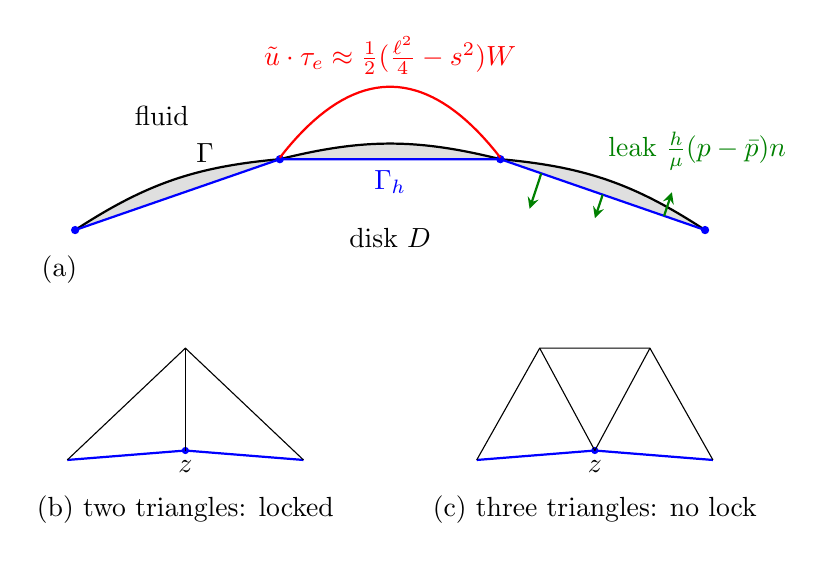
\begin{tikzpicture}[scale=1.0,>=stealth]
% (a) chords, strip and bump (schematic, curvature exaggerated)
\begin{scope}[shift={(0,0.4)}]
\coordinate (V0) at (-4,-0.9); \coordinate (V1) at (-1.4,0); \coordinate (V2) at (1.4,0); \coordinate (V3) at (4,-0.9);
\fill[gray!25] (V0) to[bend left=14] (V1) -- cycle;
\fill[gray!25] (V1) to[bend left=14] (V2) -- cycle;
\fill[gray!25] (V2) to[bend left=14] (V3) -- cycle;
\draw[thick] (V0) to[bend left=14] (V1) to[bend left=14] (V2) to[bend left=14] (V3);
\draw[thick,blue] (V0) -- (V1) -- (V2) -- (V3);
\foreach \v in {V0,V1,V2,V3} \fill[blue] (\v) circle (1.5pt);
\node at (-2.35,0.08) {$\Gamma$};
\node[blue,below] at (0,-0.02) {$\Gamma_h$};
\node at (-2.9,0.55) {fluid};
\node at (0,-1.0) {disk $D$};
% bump on the middle chord (tangential velocity profile, drawn as a graph over the chord)
\draw[red,thick,domain=-1.4:1.4,samples=40] plot (\x,{0.9*(1-(\x/1.4)^2)+0.02});
\node[red,above] at (0,0.95) {$\tilde u\cdot\tau_e\approx\tfrac12(\tfrac{\ell^2}4-s^2)W$};
% leak arrows on the right chord (normal, varying sign)
\foreach \t/\l in {0.2/0.45,0.5/0.3,0.8/-0.3} {
  \draw[->,green!50!black,thick] ($(V2)!\t!(V3)$) -- ++(-0.33*\l,-1*\l);
}
\node[green!50!black] at (3.9,0.1) {leak $\frac h\mu(p-\bar p)n$};
\node at (-4.2,-1.4) {(a)};
\end{scope}
% (b) locked vertex, two triangles
\begin{scope}[shift={(-2.6,-3.3)}]
\draw[thick,blue] (-1.5,-0.12) -- (0,0) -- (1.5,-0.12);
\fill[blue] (0,0) circle (1.3pt);
\draw (-1.5,-0.12) -- (0,1.3) -- (1.5,-0.12);
\draw (0,0) -- (0,1.3);
\node[below] at (0,0) {$z$};
\node at (0,-0.75) {(b) two triangles: locked};
\end{scope}
% (c) three triangles
\begin{scope}[shift={(2.6,-3.3)}]
\draw[thick,blue] (-1.5,-0.12) -- (0,0) -- (1.5,-0.12);
\fill[blue] (0,0) circle (1.3pt);
\draw (-1.5,-0.12) -- (-0.7,1.3) -- (0.7,1.3) -- (1.5,-0.12);
\draw (0,0) -- (-0.7,1.3); \draw (0,0) -- (0.7,1.3);
\node[below] at (0,0) {$z$};
\node at (0,-0.75) {(c) three triangles: no lock};
\end{scope}
\end{tikzpicture}
\caption{(a) The wall $\Gamma$, the inscribed polygon $\Gh$ and the thin strip between them (grey, exaggerated). On each chord the extended solution is a tangential velocity whose profile along the chord is a parabola of height $\ell^2W/8$ (the chordal bump, red), which produces Scott's $\hG^{3/2}$. The printed method adds a normal leak $(h/\mu)(p-\pbar)$ (green). (b) A polygon vertex in two triangles: divergence-free fields vanishing on both chords have zero gradient at $z$. (c) With three triangles the gradient can jump across the interior edges, and the lock disappears (Section~\ref{sec:strong}).}
\label{fig:geometry}
\end{figure}

\emph{Spaces.} Fix $k\ge4$. $\Vh$ is the space of continuous piecewise-$P_k$ vector fields on $\Th$, $\VR:=\{v\in\Vh:v|_{\partial R}=0\}$, $\VO:=\{v\in\Vh:v|_{\partial\Oh}=0\}$, $\Pih$ is the space of discontinuous piecewise-$P_{k-1}$ functions, $\Zh:=\{v\in\VR:\div v=0\}$ and $\Yh:=\Zh\cap\VO$. The discrete outer data $\gI$ are the $P_k$ Lagrange interpolant of $g$, and $\Wh:=\{z\in\Vh:z|_{\partial R}=\gI,\ \div z=0\}$.

An exactly divergence-free method is sensitive to the net flux of its Dirichlet data \cite{EickmannScottTscherpel2025}: every $z\in\Wh$ has $\int_{\Gh}z\cdot n=-\int_{\partial R}\gI\cdot\nu$ ($\nu$ the outward normal of $R$), while the exact solution has zero flux through $\Gamma$. The interpolant $\gI$ has a small nonzero flux $m_R:=\int_{\partial R}\gI\cdot\nu$, of order $h^{\sigma_k}$ with $\sigma_k=k+2$ for even $k$ and $k+1$ for odd $k$ (Newton--Cotes). It is removed by a one-line correction.

\begin{definition}[Flux-corrected outer data]\label{def:flux}
$\tilde g_I:=\gI-\dfrac{m_R}{8L^2}\,x$ on $\partial R$, where $x$ is the position field. Since $\int_{\partial R}x\cdot\nu=\int_R\div x=8L^2$, $\tilde g_I$ has zero net flux, and it is again continuous and piecewise $P_k$.
\end{definition}

\subsection{The two Nitsche methods}
With $Du=\nabla u+(\nabla u)^{\mathsf T}$, $a_h(u,v)=\frac12(Du,Dv)$ and $\dn u:=(\nabla u)n$, the symmetric Nitsche form of Gjerde and Scott is
\[
N_h(u,v)=a_h(u,v)-\ip{\dn u}{v}-\ip{u}{\dn v}+\frac{\mu}{h}\ip{u}{v}.
\]
In words: the viscous form, minus the normal flux of the solution tested against the test function (the consistency term), minus its symmetric counterpart, plus the penalty. The only piece of the Stokes traction that is represented is the viscous flux $(\nabla u)n$; the pressure traction $-pn$ is absent.

\begin{definition}[The printed method $\GS$ {\cite[(27)--(28)]{GjerdeScott2024}}]
Find $u_h\in\Vh$ with $u_h|_{\partial R}=\gI$ and $p_h\in\Pih$ such that
\[
N_h(u_h,v)-(p_h,\div v)=(\ft,v)\quad\forall v\in\VR,\qquad (q,\div u_h)=0\quad\forall q\in\Pih.
\]
\end{definition}
Here $\ft$ is a smooth extension of $f$ to the strip $S_h$. Two details of the transcription: Gjerde and Scott write the pressure form with the opposite sign (our $p_h$ is their $-p_h$), and their text defines the test space as vanishing on $\Gh$, which would remove the Nitsche terms altogether; the evident intended test space is $\VR$. The outer boundary carries strongly imposed data; the Nitsche terms act only on the polygon.

\begin{definition}[The mean-free correction $\CNS$]\label{def:cns}
As $\GS$, with the momentum equation
\begin{gather*}
N_h(u_h,v)-(p_h,\div v)+\ip{p_h-\pbG(p_h)}{v\cdot n}=(\ft,v)\quad\forall v\in\VR,\\
\pbG(q):=\frac1{|\Gh|}\int_{\Gh}q .
\end{gather*}
\end{definition}
The added term is the missing pressure traction, with the wall mean of the discrete pressure removed. It sits in the momentum row only, so the continuity row, and with it the pointwise incompressibility of $u_h$, is unchanged. Removing the mean is what makes the square system nonsingular (Proposition~\ref{prop:singular}). Methods ``with flux-corrected data'' replace $\gI$ by $\tilde g_I$.

\subsection{The exact solution on the polygonal domain}
The exact solution lives on $\Omega$, the discrete one on the larger domain $\Oh$. To compare them we extend $u$ across $\Gamma$ in a divergence-free way. Since $u\cdot n=0$ on $\Gamma$, the stream function $\psi$ with $u=\curl\psi=(\partial_y\psi,-\partial_x\psi)$ is single-valued; let $\psit$ be a smooth extension of $\psi$ to a neighbourhood of $\overline\Omega$ and put $\ut:=\curl\psit$, so $\div\ut=0$ everywhere. Let $\pt$ be a smooth extension of $p$. The extended fields satisfy the momentum equation up to a defect $F:=\ft+\Delta\ut-\nabla\pt$, which vanishes on $\Omega$ and is supported in the thin strip $S_h$.

\begin{assumption}[Smooth solution]\label{ass:D}
$(u,p)$ and $\ft$ are smooth and bounded on a fixed neighbourhood of $\overline\Omega$, and $h\le h_\ast$ is small.
\end{assumption}
Near $\Gamma$ this follows from smooth data. At the four corners of the box it is a genuine hypothesis on the \emph{solution}: for generic smooth, compatible data the Stokes velocity at a right-angled corner is only in $H^s$ for $s<3.7396$ \cite{Dauge1989}. It holds for the manufactured tests of Section~\ref{sec:numerics}. For data-driven problems on meshes that are quasi-uniform at the corners the terms $h^k$ below become $h^{\min(k,2.7396)-\epsilon}$, and the terms $h^{k+1}$ of the $L^2$ bounds degrade likewise, unless the mesh is graded there \cite{PadhiExt}. The terms involving $\hG$ are unaffected.

\emph{Norms and constants.} For fields with traces on $\Gh$ we use the mesh-dependent energy norm
\[
\tnorm{v}^2:=\norm{\nabla v}_{\Oh}^2+\frac{\mu}{h}\norm{v}_{\Gh}^2+\sum_{e\in\EG}|e|\,\norm{\dn v}_{L^2(e)}^2 .
\]
The middle term is the \emph{slip} part. We write $G:=\norm{p-\pbar}_{L^2(\Gamma)}$, where $\pbar$ is the mean of $p$ over $\Gamma$; $G=0$ exactly when the pressure is constant along the wall. Constants $C,c$ depend on (M0)--(M2), $k$, $L$ and norms of $(u,p,\psit)$, never on $h,\hG,\mu,\gamma,\rho$ unless displayed; $C_p$ may also depend on $\norm{p-\pbar}_{W^{1,\infty}(\Gamma)}$.

\subsection{Geometry of chords}
Everything that distinguishes the polygon from the circle is contained in the following elementary facts.

\begin{lemma}[Chords]\label{lem:chords}
Let $e$ be a chord of length $\ell$, $x\in e$, $s$ the signed arclength from the midpoint $m_e$ of $e$, and $x^\ast=x/|x|$ the nearest point of $\Gamma$. Then $d:=\dist(x,\Gamma)=\frac12(\frac{\ell^2}4-s^2)+O(\ell^4)$, in particular $d\le\ell^2/4$, and, up to a fixed orientation sign,
\[
n(x^\ast)-n_e=-s\,\tau_e+O(\ell^2).
\]
The arclength Jacobian of the radial projection $\Gh\to\Gamma$ is $1+O(\ell^2)$.
\end{lemma}

\begin{proof}
$|x|^2=1-\ell^2/4+s^2$. The normal at $x^\ast$ is radial, and its angle differs from that of $n_e$ by the central angle to $x^\ast$, which is $s+O(s^3)$.
\end{proof}

\begin{lemma}[Wall structure and extension]\label{lem:wall}
On $\Gamma$ we have $\nabla u=\dn u\otimes n$ and $\dn u\cdot n=0$; hence $\dn u=W\tau$ with the \emph{wall shear} $W:=\dn u\cdot\tau$. On $\Gh$, $\norm{\ut}_{L^\infty(\Gh)}\le C\hG^2$, and for $x\in e$,
\begin{equation}\label{eq:bump}
\ut(x)=d\,W(x^\ast)\tau(x^\ast)+O(d^2)=\tfrac12\bigl(\tfrac{\ell^2}4-s^2\bigr)W(m_e^\ast)\,\tau_e+O(\hG^3).
\end{equation}
Moreover $|(F,v)|\le C\hG^2\norm{\nabla v}$ for $v\in\VR$.
\end{lemma}

\begin{proof}
Tangential derivatives of $u$ vanish on $\Gamma$, and $\div u=n\cdot\dn u$. Taylor-expand $\ut$ at $x^\ast$ and use Lemma~\ref{lem:chords}. For the last bound, $F$ is bounded and supported in the strip $S_h$ of width $O(\hG^2)$; apply a one-dimensional Poincar\'e inequality across the strip and the uniform Friedrichs inequality of Lemma~\ref{lem:korn}.
\end{proof}

Formula \eqref{eq:bump} is the \emph{chordal bump}: on each chord the extended solution is a parabola of height $\ell^2W/8$ in the tangential direction. It carries the whole of Scott's $\hG^{3/2}$ (Section~\ref{sec:corrected}).

\begin{lemma}[Uniform trace, Friedrichs and Korn inequalities]\label{lem:korn}
There are $C_{\mathrm{tr}},C_F,\kappa$, independent of $h$, such that every $v\in H^1(\Oh)^2$ with $v|_{\partial R}=0$ satisfies
$\norm{v}_{L^2(\Gh)}\le C_{\mathrm{tr}}\norm{\nabla v}$, $\norm{v}\le C_F\norm{\nabla v}$ and $\norm{\nabla v}^2\le\kappa\,a_h(v,v)$.
\end{lemma}

\begin{proof}
Write $\Gh$ in polar form as $r=\rho_h(\theta)$. On a chord with endpoint angles $\theta_m\pm\alpha$, $\rho_h=\cos\alpha/\cos(\theta-\theta_m)$, so $\norm{\rho_h-1}_\infty\le C\hG^2$ and $\norm{\rho_h'}_\infty\le C\hG$. Let $\chi$ be smooth with $\chi(1)=1$ and $\chi\equiv0$ outside a fixed collar in $\Omega$, and $\Phi_h(r,\theta)=(r+\chi(r)(\rho_h(\theta)-1),\theta)$. Then $\Phi_h$ maps $\Omega$ onto $\Oh$ and $\Gamma$ onto $\Gh$, is the identity near $\partial R$, and $\norm{D\Phi_h-I}_\infty\le C\hG$. For $w=v\circ\Phi_h$ we have $D(w)=D(v)\circ\Phi_h+E$ with $|E|\le C\hG|\nabla v\circ\Phi_h|$. On the fixed domain $\Omega$ the function $w$ vanishes on $\partial R$, so Korn's first inequality, the trace inequality and Friedrichs' inequality hold there; changing variables back gives $\norm{\nabla v}\le C(\norm{D(v)}+\hG\norm{\nabla v})$, and the last term is absorbed for $\hG\le h_\ast$.
\end{proof}

The next lemma is the first place where the geometry produces the exponent $\frac32$. Its content is a cancellation: the transposed-gradient term that the symmetric-gradient form leaves on the chords is only $O(\hG)$ pointwise, but its leading part is odd in $s$ on each chord.

\begin{lemma}[Transposed-gradient term]\label{lem:transposed}
For $v\in\VR$, $|\ip{(\nabla\ut)^{\mathsf T}n}{v}|\le C\hG^{3/2}\norm{\nabla v}$.
\end{lemma}

\begin{proof}
By Taylor expansion at $x^\ast$ and Lemmas~\ref{lem:chords}--\ref{lem:wall}, $(\nabla\ut)^{\mathsf T}n_e=n(x^\ast)(\dn u(x^\ast)\cdot(n_e-n(x^\ast)))+O(\hG^2)=s\,a_e+O(\hG^2)$ on $e$, with $a_e:=n(m_e^\ast)W(m_e^\ast)$ constant on $e$. Since $\int_es\,ds=0$,
\[
\Bigl|\int_es\,a_e\cdot v\Bigr|=\Bigl|\int_es\,a_e\cdot(v-v(m_e))\Bigr|\le\frac{|e|^2}{4}\norm{\dt v}_{L^1(e)}\le C|e|^{5/2}\norm{\dt v}_{L^2(e)} .
\]
With the inverse trace inequality $|e|\norm{\dt v}_{L^2(e)}^2\le C_I^2\norm{\nabla v}^2_{T_e}$ and $\#\EG\le C/\hG$, the sum over the chords is at most $C\hG^{3/2}\norm{\nabla v}$. The remainder $O(\hG^2)$ is handled by the trace inequality of Lemma~\ref{lem:korn}.
\end{proof}

\subsection{Discrete tools}
\begin{lemma}[Inverse traces]\label{lem:inverse}
For $v\in\Vh$, $\sum_{e\in\EG}|e|\norm{\dn v}^2_{L^2(e)}\le C_I^2\norm{\nabla v}^2$, hence $\norm{\dn v}_{\Gh}\le C_I(\rho/h)^{1/2}\norm{\nabla v}$. For $q\in\Pih$, $\norm{q}^2_{\Gh}\le C_I^2(\rho/h)\norm{q}^2$.
\end{lemma}

The following lemma is the standard coercivity argument for Nitsche's method, written so that the role of $\rho$ is visible.

\begin{lemma}[Coercivity and continuity]\label{lem:coercive}
Let $\mu_0:=4\kappa\rho C_I^2$. If $\mu\ge\mu_0$ (which holds when $\gamma\ge\gamma_0:=4\kappa C_I^2/c_0$), then
\[
N_h(v,v)\ge c_1\tnorm{v}^2\quad\forall v\in\VR,\qquad |N_h(w,v)|\le M\tnorm{w}\,\tnorm{v},
\]
with $c_1,M$ independent of $h$, $\mu$ and $\rho$.
\end{lemma}

\begin{proof}
By Lemma~\ref{lem:inverse} and Young's inequality, $2|\ip{\dn v}{v}|\le\frac12a_h(v,v)+2\kappa\rho C_I^2h^{-1}\norm{v}^2_{\Gh}$. Hence $N_h(v,v)\ge\frac12a_h(v,v)+(\mu-2\kappa\rho C_I^2)h^{-1}\norm{v}^2_{\Gh}$, and for $\mu\ge\mu_0$ this is at least $(2\kappa)^{-1}\norm{\nabla v}^2+(\mu/2h)\norm{v}^2_{\Gh}$. Adding the inverse trace bound for the last part of $\tnorm\cdot$ gives coercivity. Continuity: each $\dn$-term is at most $(\rho/\mu)^{1/2}\tnorm w\tnorm v\le(4\kappa C_I^2)^{-1/2}\tnorm w\tnorm v$.
\end{proof}

Scott--Vogelius theory enters through the next two results.

\begin{lemma}[Uniform inf-sup constant]\label{lem:infsup}
There is $\beta>0$, depending only on $k$, $\Theta_0$, shape regularity and $L$, such that for every $q\in\Pih\cap L^2_0(\Oh)$ there is $v\in\VO$ with $\div v=q$ and $\norm{\nabla v}\le\beta^{-1}\norm{q}$.
\end{lemma}

\begin{proof}[Sketch]
Guzm\'an and Scott \cite[Theorem~1]{GuzmanScott2019} prove this for $k\ge4$ under (M1)--(M2), with a local Fortin construction that uses neither quasi-uniformity nor small $h$. The domain enters only through the continuous inf-sup constant and a Poincar\'e constant. The latter is uniform by Lemma~\ref{lem:korn}. For the former, cover $\Oh$ by the pieces $W_j\cap\Oh$, where the $W_j$ are fixed angular wedges about the centre of the disk; each piece is star-shaped with respect to a ball of fixed radius (every chord line meeting $W_j$ leaves the ball on its outer side, because $P_h\subset D$), and the pieces have diameters, ball radii and overlaps bounded independently of $h$. Gluing Bogovski\u{\i} operators over such a finite cover gives a uniform continuous inf-sup constant \cite{PadhiExt}. Alternatively, Bernardi, Costabel, Dauge and Girault prove directly that the continuous inf-sup constant of an inscribed polygonal approximation differs from that of the curved domain by $O(h)$ \cite[Theorem~4.6]{BCDG2016}. %% VERIFY: theorem number checked in the arXiv/author copies only, not the SIAM typeset version.
\end{proof}

\begin{lemma}[Divergence range and approximation]\label{lem:approx}
Under (M1), $\div\VR=\Pih$, $\Wh\ne\emptyset$, and the velocities of $\GS$ and $\CNS$ are divergence-free pointwise. Moreover
\[
E_h:=\inf_{z\in\Wh}\tnorm{\ut-z}\le C\eps,\qquad \eps:=(1+(\gamma\hG)^{1/2})\,h^k+h^{\sigma_k}\bigl(\hG^{-1/2}+(\mu/h)^{1/2}\bigr).
\]
With flux-corrected data the flux part $h^{\sigma_k}(\cdots)$ is replaced by $(1+\gamma^{1/2})\hG^{\sigma_k-1/2}+|m_R|$.
\end{lemma}

\begin{proof}
\emph{Divergence range.} Lemma~\ref{lem:infsup} gives $\div\VO=\Pih\cap L^2_0$. The quadratic edge bubble $b=\beta_en_e$ on a single chord lies in $\VR$ and has $\int\div b=\int_{\Gh}b\cdot n=|e|/6\ne0$; this adds the constants, so $\div\VR=\Pih$. For any $\mathcal G\in\Vh$ with trace $\gI$ on $\partial R$ we have $\div\mathcal G\in\Pih=\div\VR$, so $\mathcal G-v\in\Wh$ for a suitable $v\in\VR$. For the discrete velocity, $u_h-\mathcal G\in\VR$ and the continuity equation forces $\div u_h=0$.

\emph{Interpolation.} Let $w_h:=I_h\ut$ be the Lagrange interpolant; $w_h=\gI$ on $\partial R$. Boundary triangles have diameter at most $C\hG$, so $\norm{\nabla(\ut-w_h)}\le Ch^k$, $\norm{\ut-w_h}_{L^\infty(\Gh)}\le C\hG^{k+1}$ and $\norm{\dn(\ut-w_h)}_{L^\infty(\Gh)}\le C\hG^k$, whence $\tnorm{\ut-w_h}\le C(1+(\gamma\hG)^{1/2})h^k$. Moreover $\div w_h=\div(w_h-\ut)\in\Pih$ has norm at most $Ch^k$.

\emph{Net flux.} Since $\ut=g$ on $\partial R$ and $\div\ut=0$, $\int_{\Gh}\ut\cdot n=-\int_{\partial R}g\cdot\nu=0$, and therefore
\[
m:=\int_{\Oh}\div w_h=\int_{\partial R}(\gI-g)\cdot\nu+\int_{\Gh}(w_h-\ut)\cdot n,\qquad |m|\le Ch^{\sigma_k}.
\]
Equispaced $P_k$ interpolation on an edge integrates like the closed $(k+1)$-point Newton--Cotes rule, which is exact for polynomials of degree $\sigma_k-1$; so each edge contributes $O(|e|^{\sigma_k+1})$.

\emph{Removing the mean.} Let $b:=\sum_{e\in\EG}\beta_en_e$, so $\int\div b=|\Gh|/6$, and $a:=6m/|\Gh|$. Since $\#\EG\le C/\hG$,
$\tnorm{ab}\le C|a|(\hG^{-1/2}+(\mu/h)^{1/2})\le C\eps$, and $\norm{\div(ab)}\le C|a|\hG^{-1/2}\le C\eps$.

\emph{Divergence correction.} The field $q:=\div(w_h-ab)\in\Pih$ has mean zero and $\norm q\le C\eps$. Lemma~\ref{lem:infsup} gives $v\in\VO$ with $\div v=q$ and $\norm{\nabla v}\le C\eps$; since $v=0$ on $\Gh$, $\tnorm v\le(1+C_I^2)^{1/2}\norm{\nabla v}$. Then $z:=w_h-ab-v\in\Wh$ and $\tnorm{\ut-z}\le C\eps$.

\emph{Flux-corrected data.} Replace $w_h$ by $I_h\ut-c\,I_h(\zeta x)$ with $c=m_R/(8L^2)$ and $\zeta$ a cut-off equal to $1$ near $\partial R$ and $0$ near $\Gamma$. Its trace on $\partial R$ is $\tilde g_I$, it costs $C|m_R|$ in energy (no boundary terms on $\Gh$), and its net flux is now $\int_{\Gh}(I_h\ut-\ut)\cdot n=O(\hG^{\sigma_k})$, because only the chords contribute. The bubble step then costs $C(1+\gamma^{1/2})\hG^{\sigma_k-1/2}$.
\end{proof}

The flux term is genuine for the plain interpolant: every $z\in\Wh$, including the discrete velocity, has $\int_{\Gh}z\cdot n=-m_R$, so $\tnorm{\ut-z}\ge(\mu/h)^{1/2}|m_R|/|\Gh|^{1/2}$. For bounded $\gamma$ it is below $Ch^k$ whenever $\hG\ge h^{2(\sigma_k-k)}$ ($\hG\ge h^4$ for even $k$, $\hG\ge h^2$ for odd $k$).

\subsection{The error equation}
Testing the extended solution in the Nitsche form produces the pressure traction, which is where the two methods part ways.

\begin{lemma}[Error equation]\label{lem:erroreq}
For $v\in\VR$,
\begin{gather*}
N_h(\ut,v)-(\pt,\div v)+\ip{\pt}{v\cdot n}=(\ft,v)+\Gc(v),\\
\Gc(v):=\ip{(\nabla\ut)^{\mathsf T}n}{v}-\ip{\ut}{\dn v}+\frac\mu h\ip{\ut}{v}-(F,v),
\end{gather*}
and $|\Gc(v)|\le C(1+\gamma^{1/2})\hG^{3/2}\tnorm v$; for $v\in\VO$, $|\Gc(v)|\le C\hG^{3/2}\norm{\nabla v}$.
\end{lemma}

\begin{proof}
Since $D(\ut)$ is symmetric and $v=0$ on $\partial R$, $a_h(\ut,v)=-(\div D(\ut),v)+\ip{D(\ut)n}{v}$, and $\div D(\ut)=\Delta\ut$ because $\div\ut=0$. Insert $-\Delta\ut=\ft-F-\nabla\pt$, integrate $-(\nabla\pt,v)=(\pt,\div v)-\ip{\pt}{v\cdot n}$ by parts, and use $D(\ut)n-\dn\ut=(\nabla\ut)^{\mathsf T}n$. For the bound: the transposed term is Lemma~\ref{lem:transposed}; $|\ip{\ut}{\dn v}|\le C\hG^2\cdot C_I(\rho/h)^{1/2}\norm{\nabla v}\le C\hG^{3/2}\norm{\nabla v}$; the penalty term is at most $(\mu/h)^{1/2}C\hG^2\tnorm v=C\gamma^{1/2}\hG^{3/2}\tnorm v$; and the $F$-term is Lemma~\ref{lem:wall}. For $v\in\VO$ the transposed and penalty terms vanish.
\end{proof}

The functional $\Gc$ is the geometric consistency error, common to both methods and of Scott's order $\hG^{3/2}$. For $\GS$ the error equation has one more term. Testing with divergence-free $v\in\Zh$, which have zero net flux through $\Gh$, we can subtract any constant from the pressure:

\begin{corollary}[The printed method on divergence-free test functions]\label{cor:GSerr}
For $v\in\Zh$ and every constant $c$,
\[
N_h(\ut-u_h,v)=\Rc(v)+\Gc(v),\qquad \Rc(v):=-\ip{\pt-c}{v\cdot n}.
\]
\end{corollary}
We will take $c=\pbar$. The functional $\Rc$ is the \emph{missing traction}. It is of size $G$, not small, and it is the subject of the next section.

\subsection{A roadmap of the error analysis}
All the upper bounds below are built from the same three ingredients, and it may help to see them side by side before the details.
\begin{enumerate}[label=(\roman*)]
\item \emph{Approximation.} How well can divergence-free discrete fields with the right outer data approximate the extended solution? Lemma~\ref{lem:approx} answers: to within $\eps$, which is $h^k$ plus a flux term that the flux-corrected data remove. This is where Scott--Vogelius theory (Lemma~\ref{lem:infsup}) and the angle condition (M2) enter.
\item \emph{Geometric consistency.} The extended solution does not vanish on the chords; it has the chordal bump \eqref{eq:bump} of height $O(\hG^2)$. Every Nitsche term that sees this trace produces a consistency error, collected in $\Gc$, of order $\hG^{3/2}$ (Lemma~\ref{lem:erroreq}); the exponent $\frac32$ comes either from odd symmetry on each chord (Lemma~\ref{lem:transposed}) or from the $H^{1/2}$ size of the bump. This error is common to all methods that impose the wall condition on the polygon, weakly or strongly, and it is sharp (Theorems~\ref{thm:lb} and~\ref{thm:st:low}).
\item \emph{Traction consistency.} For $\GS$ the missing traction $\Rc$ is an additional consistency error of order one, which the penalty converts into the leak of size $h/\mu$ (Section~\ref{sec:printed}). For $\CNS$ it is absent, but the pressure now enters the velocity estimate through the wall term, and it has to be controlled by the inf-sup condition and absorbed, which is why $\CNS$ needs $\gamma\ge\gamma_2$ (Theorem~\ref{thm:D}).
\end{enumerate}
The lower bounds use test fields tailored to each error: a divergence-free field with normal trace $-(p-\pbar)n$ for the leak (Section~\ref{sec:printed}), divergence-free fields vanishing on the wall and feeling the second moment of the bump for the geometric error (Section~\ref{sec:lb}), and local vertex-gradient arguments for strong imposition (Section~\ref{sec:strong}).

\section{The printed method: the leak law}\label{sec:printed}

\emph{Relation to \cite{CavalcantePadhiLetter}.} Theorems~\ref{thm:A}, \ref{thm:C} and~\ref{thm:B} and Corollary~\ref{cor:Bp} were announced in the joint letter \cite{CavalcantePadhiLetter}, with proof sketches; we give complete proofs here. The identification of the $H^1$ constant with a Stokes leak flow (Section~\ref{sec:leakflow}) is not in the letter.

Throughout this section $u_h$ is the velocity of $\GS$ and $\gamma\ge\gamma_0$, so that $N_h$ is coercive (Lemma~\ref{lem:coercive}). The error equation of Corollary~\ref{cor:GSerr} has two right-hand sides. The geometric part $\Gc$ is of Scott's order. The traction part $\Rc(v)=-\ip{\pt-\pbar}{v\cdot n}$ is of order one; it is a normal load on the wall, and the only term of $N_h$ that can balance a normal load of order one on the wall is the penalty. This suggests that $u_h$ carries a normal wall velocity $(h/\mu)(p-\pbar)$. We now make this precise: first in the energy norm, where the leak is seen directly, then in the $H^1$ seminorm, where incompressibility improves the rate, and finally at the level of the exact leading term and its $H^1$ constant.

\subsection{A divergence-free field with prescribed normal trace}
All lower bounds need a discrete divergence-free field whose trace on the wall looks like the leak. Let
\[
\varphi_0(\theta):=\int_0^\theta(p-\pbar)(\theta')\,d\theta',
\]
which is periodic because $p-\pbar$ has zero mean on $\Gamma$, and let $\varphi:=\chi_1(r)\varphi_0(\theta)$ with a cut-off $\chi_1$ equal to $1$ near $r=1$ and $0$ near $\partial R$. Then $w:=\curl\varphi$ satisfies
\[
w=(p-\pbar)e_r=-(p-\pbar)\,n\qquad\text{on }\Gamma .
\]
Let $\Pi_{k+1}$ be the $C^1$ piecewise-$P_{k+1}$ interpolant of Morgan and Scott \cite{MorganScott1975} (for $k=4$, the Argyris interpolant \cite{Argyris1968}); it exists because $k+1\ge5$. The field $v_\varphi:=\curl\Pi_{k+1}\varphi$ is continuous, piecewise $P_k$, divergence-free and vanishes near $\partial R$, so $v_\varphi\in\Zh$, and $\norm{v_\varphi-w}_{W^{1,\infty}}\le Ch^k$.

\subsection{The energy norm: rate exactly one half}

\begin{theorem}[Energy error of the printed method; announced in {\cite{CavalcantePadhiLetter}}]\label{thm:A}
The error of $\GS$ satisfies
\[
\tnorm{\ut-u_h}\le C\Bigl[(h/\mu)^{1/2}G+(1+\gamma^{1/2})\hG^{3/2}+\eps\Bigr].
\]
If $G>0$ and $h\le h_0(G)$, with $h_0$ independent of $\gamma\ge\gamma_0$, then also
\[
\tnorm{\ut-u_h}\ge(2M)^{-1}(h/\mu)^{1/2}G-C\Bigl[(1+\gamma^{1/2})\hG^{3/2}+\eps\Bigr].
\]
In particular, for $G=0$ the printed method satisfies $\tnorm{\ut-u_h}\le C[(1+\gamma^{1/2})\hG^{3/2}+\eps]$, which is Scott's expected estimate.
\end{theorem}

\begin{proof}
\emph{Upper bound.} For $z\in\Wh$ the difference $e_h:=z-u_h$ lies in $\Zh$. By Corollary~\ref{cor:GSerr} and Lemma~\ref{lem:coercive},
\[
c_1\tnorm{e_h}^2\le N_h(z-\ut,e_h)+\Rc(e_h)+\Gc(e_h).
\]
With the Jacobian bound of Lemma~\ref{lem:chords}, $|\Rc(e_h)|\le(G+C\hG^2)\norm{e_h}_{\Gh}\le(G+C\hG^2)(h/\mu)^{1/2}\tnorm{e_h}$. Lemmas~\ref{lem:erroreq} and~\ref{lem:approx} bound the other two terms.

\emph{Lower bound.} On a chord, $v_\varphi\cdot n_e=-(p-\pbar)(x^\ast)\,n(x^\ast)\cdot n_e+O(h^k)$ and $n(x^\ast)\cdot n_e=1+O(s^2)$, so
\[
\Rc(v_\varphi)=G^2+O(\hG^2+h^k),\qquad \tnorm{v_\varphi}^2\le\frac\mu h\bigl(G+C\hG^2+Ch^k\bigr)^2+C .
\]
By continuity of $N_h$, $M\tnorm{\ut-u_h}\ge(|\Rc(v_\varphi)|-|\Gc(v_\varphi)|)/\tnorm{v_\varphi}$, and the quotient $|\Rc(v_\varphi)|/\tnorm{v_\varphi}$ is at least $\frac12(h/\mu)^{1/2}G$ once $h\le h_0(G)$.
\end{proof}

The lower bound is carried by the slip part $(\mu/h)^{1/2}\norm{\cdot}_{\Gh}$ of the energy norm. When $G>0$, $\gamma\hG\ll G$ and $\eps\ll(h/\mu)^{1/2}G$, the energy error is therefore $\asymp(h/\mu)^{1/2}$: the energy rate is exactly $\frac12$. The $H^1$ seminorm behaves better.

\subsection{The \texorpdfstring{$H^1$}{H1} seminorm: incompressibility turns a normal load into a tangential derivative}
A normal velocity of size $h/\mu$ on the chords, lifted into the domain by a generic discrete field, costs $(h/\mu)\hG^{-1/2}$ in $H^1$, because the lift oscillates on the element scale. The following lemma shows that divergence-free fields do not pay this price for \emph{normal} loads.

\begin{lemma}[Normal-load cancellation]\label{lem:cancel}
Let $S$ be edgewise $W^{1,\infty}$ on $\Gh$, continuous at the vertices of $\Gh$, with $|S\cdot\tau_e|\le C\hG$ on every $e\in\EG$ (for instance $S$ smooth with $S\cdot\tau=0$ on $\Gamma$). Then for $v\in\Zh$,
\[
|\ip{S}{\dn v}|\le C\bigl(\norm{v}_{\Gh}+\hG^{1/2}\norm{\nabla v}\bigr)\le C\norm{\nabla v}.
\]
\end{lemma}

\begin{proof}
The tangential part of $S$ is small: $|\ip{(S\cdot\tau)\tau}{\dn v}|\le C\hG\norm{\dn v}_{\Gh}\le C\hG^{1/2}\norm{\nabla v}$ by Lemma~\ref{lem:inverse} and (M0). For the normal part, $v$ is a polynomial on the triangle $T_e$ with $\div v=0$, so on $e$
\[
\dn v\cdot n_e=\dn(v\cdot n_e)=-\dt(v\cdot\tau_e).
\]
With $\sigma_e:=S\cdot n_e$, integration by parts along the chord gives
\[
\int_e\sigma_e\,\dn v\cdot n_e=\int_e\dt\sigma_e\,(v\cdot\tau_e)-\bigl[\sigma_e\,v\cdot\tau_e\bigr]_{\partial e}.
\]
At a polygon vertex $x$ shared by $e$ and $e'$ the endpoint terms combine to $v(x)\cdot(\sigma_{e'}\tau_{e'}-\sigma_e\tau_e)$, which is of size $C(|e|+|e'|)|v(x)|$ because $S$ is continuous and the chords turn by $O(\hG)$. Summing, $\sum_e|e|\norm{v}_{L^\infty(e)}\le C|\Gh|^{1/2}\norm{v}_{\Gh}$, and Lemma~\ref{lem:korn} finishes.
\end{proof}

Computations confirm that this is exactly what incompressibility buys: the discrete dual norm of $v\mapsto\ip{S}{\dn v}$ stays bounded on $\Zh$ for normal $S$, but grows like $\hG^{-1/2}$ on $\VR$ and also on $\Zh$ for tangential $S$ (Table~\ref{tab:lemma}).

\begin{theorem}[$H^1$ error of the printed method; announced in {\cite{CavalcantePadhiLetter}}]\label{thm:C}
With $C_p:=C(1+\norm{p-\pbar}_{W^{1,\infty}(\Gamma)})$,
\[
\norm{\nabla(\ut-u_h)}\le C_p\,\frac h\mu+C\Bigl[(1+\gamma^{1/2})\hG^{3/2}+\eps\Bigr].
\]
\end{theorem}

\begin{proof}
\emph{Split.} For $z\in\Wh$ write $z-u_h=\delta_R+\delta_G$ with $\delta_R,\delta_G\in\Zh$ defined by
\[
N_h(\delta_R,v)=\Rc(v),\qquad N_h(\delta_G,v)=\Gc(v)-N_h(\ut-z,v)\qquad\forall v\in\Zh .
\]
The geometric part is bounded in energy by coercivity: $\norm{\nabla\delta_G}\le\tnorm{\delta_G}\le C(1+\gamma^{1/2})\hG^{3/2}+CE_h$.

\emph{Ansatz for the traction part.} We expect $\delta_R\approx(h/\mu)w$, with $w=-(p-\pbar)n$ on the wall. Put $r_h:=\delta_R-(h/\mu)v_\varphi\in\Zh$. Then $N_h(r_h,v)=m(v)+\ell(v)$ with
\[
m(v):=-\ip{(\pt-\pbar)n+v_\varphi}{v},\qquad
\ell(v):=-\frac h\mu\bigl[a_h(v_\varphi,v)-\ip{\dn v_\varphi}{v}-\ip{v_\varphi}{\dn v}\bigr].
\]
The penalty applied to $(h/\mu)v_\varphi$ has cancelled the traction up to the mismatch $m$.

\emph{The mismatch.} On a chord, $(\pt-\pbar)n_e+v_\varphi=(p-\pbar)(x^\ast)(n_e-n(x^\ast))+O(\hG^2+h^k)=(p-\pbar)(m_e^\ast)\,s\,\tau_e+O(\hG^2+h^k)$. The leading term is odd in $s$ with constant coefficient, and the argument of Lemma~\ref{lem:transposed} gives $|m(v)|\le C_p(\hG^{3/2}+h^k)\norm{\nabla v}$.

\emph{The remaining terms.} $|a_h(v_\varphi,v)|+|\ip{\dn v_\varphi}{v}|\le C_p\norm{\nabla v}$. The dangerous term is $\ip{v_\varphi}{\dn v}$, which a trace-inverse estimate would bound only by $\hG^{-1/2}\norm{\nabla v}$. But $v_\varphi$ is within $Ch^k$ of the normal field $w$, so Lemma~\ref{lem:cancel} applies:
\[
|\ip{v_\varphi}{\dn v}|\le|\ip{w}{\dn v}|+|\ip{v_\varphi-w}{\dn v}|\le C_p\norm{\nabla v}+Ch^k\hG^{-1/2}\norm{\nabla v}.
\]
Hence $|\ell(v)|\le(h/\mu)(C_p+Ch^k\hG^{-1/2})\norm{\nabla v}$.

\emph{Close.} Testing with $v=r_h$ and using $(h/\mu)h^k\hG^{-1/2}=\gamma^{-1}h^k\hG^{1/2}\le Ch^k$,
\[
\norm{\nabla\delta_R}\le\frac h\mu\norm{\nabla v_\varphi}+\norm{\nabla r_h}\le C_p\frac h\mu+C(\hG^{3/2}+\eps).
\]
Collect $\ut-u_h=(\ut-z)+\delta_R+\delta_G$.
\end{proof}

\begin{remark}[Why rate one and not one half]
Without incompressibility Lemma~\ref{lem:cancel} would give only $C\hG^{-1/2}$, and the $H^1$ error would be $(h/\mu)\hG^{-1/2}$, with an element-scale oscillation in the trace. The inconsistency $-pn$ is purely \emph{normal}, and $\div v=0$ converts $\dn v\cdot n$ into a tangential derivative, which can be moved onto the smooth load. This is why the printed method still converges at rate $1$ in $H^1$.
\end{remark}

The rate $h/\mu$ is sharp. The next theorem shows that, as long as the traction term dominates, the slip is of size exactly $(h/\mu)G$, and the $H^1$ error cannot be smaller.

\begin{theorem}[Slip and $H^1$ lower bounds; announced in {\cite{CavalcantePadhiLetter}}]\label{thm:B}
Let $G>0$ and let $X:=C_p(h/\mu)+(1+\gamma^{1/2})\hG^{3/2}+\eps$ be the bound of Theorem~\ref{thm:C}. Suppose that, for a fixed small $\delta$,
\[
X\le\delta\,G\min(G,\hG^{1/2}),\qquad h/\mu\le\delta G,\qquad \hG\le h_0(G),
\]
which holds for fixed $\gamma$ and bounded $\rho$ as $\hG\to0$. Then
\[
c\,\frac h\mu G\le\norm{\ut-u_h}_{L^2(\Gh)}\le\Bigl(\frac h\mu\Bigr)^{1/2}\tnorm{\ut-u_h},\qquad
\norm{\nabla(\ut-u_h)}\ge c\,\frac h\mu G-Ch^{k+1/2}.
\]
Together with Theorem~\ref{thm:C}, $\norm{\nabla(\ut-u_h)}\asymp h/\mu$ in this regime.
\end{theorem}

\begin{proof}
Let $e_u:=\ut-u_h$ and $v:=v_\varphi$. Corollary~\ref{cor:GSerr} rearranges to
\[
\frac\mu h\ip{e_u}{v}=\Rc(v)+\Gc(v)-a_h(e_u,v)+\ip{\dn e_u}{v}+\ip{e_u}{\dn v}.
\]
We bound the five terms on the right, using that $v$ is smooth up to $O(h^k)$.
\begin{enumerate}
\item $\Rc(v)=G^2+O(\hG^2+h^k)$, as in the proof of Theorem~\ref{thm:A}.
\item $|\Gc(v)|\le C(\hG^{3/2}+\gamma\hG^3+\gamma\hG h^k)$. The only term that could be large is the penalty part $(\mu/h)\ip{\ut}{v}$; but on the chords $\ut$ is tangential to leading order (the chordal bump \eqref{eq:bump}) while $v\approx-(p-\pbar)n$ is normal, so $\ut\cdot v=O(\hG^4+\hG^2h^k)$.
\item $|a_h(e_u,v)|\le C_p\norm{\nabla e_u}\le C_pX\le C_p\delta G^2$ by Theorem~\ref{thm:C}.
\item By Theorem~\ref{thm:A} and $h/\mu\le\delta G$, $|\ip{e_u}{\dn v}|\le C_p\norm{e_u}_{\Gh}\le C_p(h/\mu)^{1/2}\tnorm{e_u}\le C_p[(h/\mu)G+X]\le2C_p\delta G^2$.
\item Split $e_u=(\ut-z)+(z-u_h)$ with $z\in\Wh$ from Lemma~\ref{lem:approx}; by Lemma~\ref{lem:inverse}, $|\ip{\dn e_u}{v}|\le\norm{\dn(\ut-z)}_{\Gh}\norm{v}_{\Gh}+C(\rho/h)^{1/2}(\norm{\nabla(z-\ut)}+\norm{\nabla e_u})\norm{v}_{\Gh}\le C\hG^{-1/2}XG\le C\delta G^2$.
\end{enumerate}
For $\delta$ small, $|\ip{e_u}{v}|\ge\frac12(h/\mu)G^2$. Dividing by $\norm{v}_{\Gh}\le G+C\hG^2$ gives the lower bound for the slip; the upper bound is the definition of $\tnorm\cdot$. For the $H^1$ bound, let $E\in H^1(\Oh)$ lift $(g-\gI)|_{\partial R}$ with $E|_{\Gh}=0$ and $\norm{E}_{H^1}\le Ch^{k+1/2}$; Lemma~\ref{lem:korn} applied to $e_u-E$ gives $\norm{e_u}_{\Gh}\le C_{\mathrm{tr}}(\norm{\nabla e_u}+\norm{\nabla E})$.
\end{proof}

\subsection{The leading term}
We can now identify the error itself, not only its size.

\begin{corollary}[Exact leading term; announced in {\cite{CavalcantePadhiLetter}}]\label{cor:Bp}
Let $G>0$ and let $\hG\to0$ with $h/\mu\to0$, $\gamma\hG\to0$ and $\eps/(h/\mu)^{1/2}\to0$ (for example $\gamma$ fixed, $\rho$ bounded). Then
\[
\ut-u_h=\frac h\mu\,v_\varphi+\vartheta_h,\qquad \tnorm{\vartheta_h}=o\bigl((h/\mu)^{1/2}\bigr),\qquad \norm{\vartheta_h}_{\Gh}=o(h/\mu),
\]
and consequently
\[
\frac{\norm{\ut-u_h}_{L^2(\Gh)}}{(h/\mu)\,G}\longrightarrow1,\qquad\frac{\tnorm{\ut-u_h}}{(h/\mu)^{1/2}G}\longrightarrow1 .
\]
\end{corollary}

\begin{proof}
In the notation of the proof of Theorem~\ref{thm:C}, $\ut-u_h=(\ut-z)+(h/\mu)v_\varphi+r_h+\delta_G$. The same energy argument gives $\tnorm{r_h}\le C_p(h/\mu+\hG^{3/2})+C\eps$, and $\tnorm{\delta_G}+\tnorm{\ut-z}\le C[(1+\gamma^{1/2})\hG^{3/2}+\eps]$; on $\Gh$ each of these carries the extra factor $(h/\mu)^{1/2}$. Relative to $(h/\mu)^{1/2}G$ and $(h/\mu)G$ they are $o(1)$ under the hypotheses. Finally $\norm{v_\varphi}_{\Gh}=G(1+O(\hG^2))+O(h^k)$ and $\tnorm{v_\varphi}^2=(\mu/h)\norm{v_\varphi}^2_{\Gh}+O(1)$.
\end{proof}

Since $v_\varphi\approx-(p-\pbar)n$ on $\Gh$, the printed method replaces the no-slip condition by the leak condition
\[
\frac\mu h\,u_h\cdot n\approx p-\pbar\qquad\text{on }\Gh,
\]
with universal constant $1$ in the slip and energy norms (Figure~\ref{fig:leak}). The leak does not change the total mass: since $\int_\Gamma(p-\pbar)=0$, the fluid that leaves through the parts of the wall where the pressure is above its mean re-enters where it is below, and the net flux through $\Gh$ is exactly that dictated by the outer data. What is violated is the local no-penetration condition, by an amount proportional to the local excess pressure. The picture is that of a slightly porous wall whose permeability is $h/\mu$; as $h\to0$ with $\mu$ fixed, the wall becomes impermeable at rate $h$. This is the sharp answer to Scott's question for the printed method: \emph{the estimate $\hG^{3/2}+h^k$ holds if and only if $p$ is constant on $\Gamma$}, and otherwise the error is the explicit leak field.

\subsection{The \texorpdfstring{$H^1$}{H1} constant is a Stokes flow}\label{sec:leakflow}
Corollary~\ref{cor:Bp} identifies the slip and energy constants but not the $H^1$ constant $\norm{\nabla(\ut-u_h)}\mu/(hG)$, because the remainder $r_h$ has the same $H^1$ order as $(h/\mu)v_\varphi$. The correct $H^1$ description is global: the leak drives a Stokes flow in the whole domain.

\begin{definition}[Leak flow]\label{def:leak}
Let $(U,P)$ solve $-\Delta U+\nabla P=0$, $\div U=0$ in $\Omega$, with $U=-(p-\pbar)n$ on $\Gamma$ and $U=0$ on $\partial R$, and put $K:=\norm{\nabla U}_{L^2(\Omega)}/G$.
\end{definition}

The data are compatible ($\int_\Gamma U\cdot n=0$), and $U$ minimises the Dirichlet energy among divergence-free fields with these boundary values. In particular $K$ depends on $p|_\Gamma$ \emph{and} on the outer boundary.

\begin{theorem}[The leak flow is the $H^1$ limit]\label{thm:hc}
Let $\tilde U$ be a smooth divergence-free extension of $U$ across $\Gamma$. For $\GS$ with $\gamma\ge\gamma_0$,
\[
\begin{aligned}
\Bigl\|\nabla\Bigl(\frac\mu h(\ut-u_h)-\tilde U\Bigr)\Bigr\|_{\Oh}&\le C_U\Bigl[\min\bigl(\gamma\hG^{1/2},(\gamma\hG)^{1/2}\bigr)+\hG^{1/2}+(h/\mu)^{1/2}+E_U\Bigr]\\
&\quad+C\frac\mu h\Bigl[(1+\gamma^{1/2})\hG^{3/2}+\eps\Bigr],
\end{aligned}
\]
where $E_U:=h+(1+(\gamma\hG)^{1/2})h^k+(1+\gamma^{1/2})\hG^{\sigma_k-1/2}$ is an approximation error for $\tilde U$ and $C_U$ depends on norms of $p$ and $U$ near $\Gamma$.
Consequently, if $\hG\to0$ with $h/\mu\to0$, $\gamma\hG\to0$, $\gamma(1+\gamma^{1/2})\hG^{1/2}\to0$ and $(\mu/h)\eps\to0$ (all of which hold for fixed $\gamma$ and bounded $\rho$),
\[
\frac{\norm{\nabla(\ut-u_h)}}{(h/\mu)\,G}\longrightarrow K .
\]
\end{theorem}

\begin{proof}
We treat the traction response $\delta_R$ of the proof of Theorem~\ref{thm:C}; the rest of the error, $(\ut-z)+\delta_G$, is bounded in energy by $C[(1+\gamma^{1/2})\hG^{3/2}+\eps]$, which after multiplication by $\mu/h$ is the last term of the bound. By a variant of Lemma~\ref{lem:approx} (with $g=0$ and only $H^2$ regularity of $U$ away from $\Gamma$) there is $z_U\in\Zh$ with $\tnorm{\tilde U-z_U}\le CE_U$. Put $\epsilon:=\delta_R-(h/\mu)z_U\in\Zh$. For $v\in\Zh$,
\[
N_h(\epsilon,v)=\Rc(v)-\frac h\mu N_h(\tilde U,v)+\frac h\mu N_h(\tilde U-z_U,v).
\]
\emph{Green's formula for $\tilde U$.} Let $\tilde P$ extend $P$ and $F_U:=-\Delta\tilde U+\nabla\tilde P$, which vanishes on $\Omega$, is bounded and is supported in the strip. As in Lemma~\ref{lem:erroreq}, since $\div v=0$, $v|_{\partial R}=0$ and $\int_{\Gh}v\cdot n=0$,
\[
N_h(\tilde U,v)=(F_U,v)+\ip{\sigma_U}{v}-\ip{\tilde U}{\dn v}+\frac\mu h\ip{\tilde U}{v},\qquad\sigma_U:=(\nabla\tilde U)^{\mathsf T}n-(\tilde P-c)n .
\]
\emph{Cancellation of the penalty terms.} With $\Rc(v)=-\ip{(\pt-\pbar)n}{v}$ the error equation becomes
\begin{gather*}
N_h(\epsilon,v)=-\ip{\zeta}{v}-\frac h\mu\Bigl[(F_U,v)+\ip{\sigma_U}{v}-\ip{\tilde U}{\dn v}\Bigr]+\frac h\mu N_h(\tilde U-z_U,v),\\
\zeta:=(\pt-\pbar)n+\tilde U .
\end{gather*}
\emph{The mismatch.} Since $\tilde U(x^\ast)=-(p-\pbar)(x^\ast)n(x^\ast)$, Lemma~\ref{lem:chords} gives $\zeta=(p-\pbar)(m_e^\ast)\,s\,\tau_e+O(\hG^2)$ on each chord, odd in $s$ to leading order. As in Lemma~\ref{lem:transposed}, $|\ip{\zeta}{v}|\le C\hG^{3/2}\norm{\nabla v}$; alternatively $\norm{\zeta}_{\Gh}\le C\hG$ gives $|\ip{\zeta}{v}|\le C\hG(h/\mu)^{1/2}\tnorm v$.

\emph{The $O(h/\mu)$ terms.} $|(F_U,v)|\le C\hG^2\norm{\nabla v}$ and $|\ip{\sigma_U}{v}|\le C(h/\mu)^{1/2}\tnorm v$. On the chords $\tilde U$ is continuous at the vertices and nearly normal, $\tilde U\cdot\tau_e=O(\hG)$, so Lemma~\ref{lem:cancel} applies to $S=\tilde U$ and $|\ip{\tilde U}{\dn v}|\le C((h/\mu)^{1/2}+\hG^{1/2})\tnorm v$. Finally $|N_h(\tilde U-z_U,v)|\le ME_U\tnorm v$.

\emph{Close.} Testing with $v=\epsilon$,
\[
c_1\tnorm{\epsilon}\le C\Bigl[\min\bigl(\hG^{3/2},\hG(h/\mu)^{1/2}\bigr)+\frac h\mu\bigl(\hG^2+(h/\mu)^{1/2}+\hG^{1/2}+E_U\bigr)\Bigr].
\]
Divide by $h/\mu$, using $\hG^{3/2}\mu/h=\gamma\hG^{1/2}$ and $\hG(\mu/h)^{1/2}=(\gamma\hG)^{1/2}$, and add $\tnorm{\tilde U-z_U}$. For the limit, multiply out and use $\norm{\nabla\tilde U}^2_{\Oh}-\norm{\nabla U}^2_\Omega=O(\hG^2)$.
\end{proof}

Two by-products of the proof are worth recording. First, on the pure-pressure test ($u=0$, $f=\nabla p$) we have $\ut=0$ and $\Gc\equiv0$, so the error of $\GS$ is exactly $\delta_R$ and the theorem applies with no further condition. Second, the remainder $r_h=\delta_R-(h/\mu)v_\varphi$ of Theorem~\ref{thm:C} satisfies $(\mu/h)r_h\to U-w$ in $H^1$: it is the Stokes correction of the cut-off field $w$, which explains why $r_h$ has the same $H^1$ order as the explicit term.

\begin{remark}[The Dirichlet-dominated regime]
The hypothesis $\gamma\hG=\mu\hG^2/h\to0$ of Corollary~\ref{cor:Bp} fails for very large penalties (for example $\gamma\hG\approx240$ at $N=96$, $\mu=10^4$). There the discrete problem is close to its $\mu\to\infty$ limit, a discrete Dirichlet problem whose data $-(p-\pbar)n_e$ jump in direction at every polygon vertex. Theorem~\ref{thm:hc} does not cover this regime, but the penalty-uniform analysis of \cite{PadhiExt} does (Section~\ref{sec:further}): the scaled traction response still converges to $U$ in $H^1$, at the exact rate $\hG^{1/2}$.
\end{remark}

\subsubsection*{Computing $K$}
The constant is a property of the continuous problem, and it can be bracketed rigorously. For $\varrho>1$ let $\mathcal A_\varrho=\{1<r<\varrho\}$ and let $\mathcal E(\varrho)$ be the minimal Dirichlet energy of divergence-free fields on $\mathcal A_\varrho$ with the leak data on $r=1$ and zero data on $r=\varrho$. Extending by zero shows that the minimum decreases as the domain grows.

\begin{proposition}[Annulus bracket]\label{prop:bracket}
If $\mathcal A_{\varrho_1}\subset\Omega\subset\mathcal A_{\varrho_2}$, then $\mathcal E(\varrho_2)\le\norm{\nabla U}^2\le\mathcal E(\varrho_1)$. In the annulus the Fourier modes decouple: if $\Psi|_\Gamma=\sum_n(a_n\cos n\theta+b_n\sin n\theta)$ is the boundary stream function of the leak, then $\mathcal E(\varrho)=\sum_n(a_n^2+b_n^2)E_n(\varrho)$ with
\[
E_n(\varrho)=\pi\int_1^\varrho\Bigl[f''^2+2n^2\bigl((f/r)'\bigr)^2+\bigl(f'/r-n^2f/r^2\bigr)^2\Bigr]r\,dr,
\]
where $f$ is the combination of $r^n,r^{-n},r^{n+2},r^{2-n}$ (of $r,r^{-1},r^3,r\log r$ for $n=1$) with $f(1)=1$, $f'(1)=0$ and $f(\varrho)=f'(\varrho)=0$.
\end{proposition}

For the pressure of test P, $p-\pbar=-\frac34\sin\theta+\frac14\sin3\theta+\frac12\cos\theta$ on $\Gamma$, so $\Psi|_\Gamma=\frac34\cos\theta+\frac12\sin\theta-\frac1{12}\cos3\theta$ and $G^2=7\pi/8$. With $\varrho_1=L=2.5$ and $\varrho_2=L\sqrt2$ the proposition gives the rigorous bracket $2.0746004\le K\le3.0525769$. The exact value on the box is computed by a series in the odd Fourier modes (imposing the outer conditions by least squares at $16\,000$ points); it is stable to eight digits under refinement of both the truncation and the quadrature:
\begin{center}\small
\begin{tabular}{rccc}
\toprule
number of modes $n_{\max}$ & max boundary residual & $\norm{\nabla U}$ & $K$\\
\midrule
15 & $4.4\cdot10^{-3}$ & 4.57012143 & 2.75644148\\
31 & $6.1\cdot10^{-5}$ & 4.57024239 & 2.75651444\\
47 & $5.1\cdot10^{-6}$ & 4.57024449 & 2.75651571\\
79 & $1.8\cdot10^{-7}$ & 4.57024450 & 2.75651571\\
\bottomrule
\end{tabular}
\end{center}
The same formulas describe the dependence on the box. As $\varrho\to\infty$, $E_3(\varrho)\to45\pi$ and $E_1(\varrho)\to\pi$; the $n=1$ data split into a potential dipole, whose exterior energy is exactly $\pi$, and a rigid translation, whose energy vanishes as the box grows (the Stokes paradox). Hence
\[
K(L)\longrightarrow\sqrt{\frac{(\frac9{16}+\frac14)\pi+\frac{45\pi}{144}}{7\pi/8}}=\frac3{\sqrt7}\approx1.134\qquad(L\to\infty),
\]
but only logarithmically: in annuli the values are $1.420$, $1.242$, $1.183$ at $\varrho=10,10^2,10^4$ (the logarithmic rate is observed, not proved).

So the constant $2.7$--$2.8$ observed in Table~\ref{tab:P} belongs to the box, not to the method. The approach to $K$ is pre-asymptotic at moderate penalties: at $\mu=100$ the measured constants increase towards $K$, at large $\mu$ they decrease towards it, and on test P the relative distance $\norm{\nabla((\mu/h)(\ut-u_h)-\tilde U)}/\norm{\nabla U}$ decays at the exact rate $\hG^{1/2}$ for every penalty, the Dirichlet limit $\mu\to\infty$ included (Section~\ref{sec:further}).

\section{The corrected method: Scott's rate and its sharpness}\label{sec:corrected}

\subsection{Why the plain pressure term fails}
Adding the missing traction $\ip{p_h}{v\cdot n}$ to the momentum equation looks like the natural repair. With an exactly divergence-free pair it makes the square system singular, and the usual way of removing the singularity destroys exact incompressibility.

\begin{proposition}[The naive consistent form and its mean-zero variant]\label{prop:singular}
\begin{enumerate}[label=(\alph*)]
\item Replace $\ip{p_h-\pbG(p_h)}{v\cdot n}$ in $\CNS$ by $\ip{p_h}{v\cdot n}$. The resulting square system has the kernel vector $(u,p)=(0,1)$, so it is singular and solvable only under one linear compatibility condition on the data.
\item Restrict the pressure to $\Pih\cap L^2_0(\Oh)$ and test the continuity equation only with mean-zero $q$. Any solution has $\div u_h\equiv c$, a constant with
\[
c\,|\Oh|=\int_{\partial R}\gI\cdot\nu+\int_{\Gh}u_h\cdot n .
\]
\item For $\gamma\ge\gamma_2$ (Theorem~\ref{thm:D}) the naive system of (a) is solvable if and only if the $\CNS$ pressure has zero mean on $\Gh$, and then its solutions are the $\CNS$ solution up to a constant pressure.
\end{enumerate}
\end{proposition}

\begin{proof}
(a) For $v\in\VR$, $-(1,\div v)+\ip{1}{v\cdot n}=-\int_{\partial\Oh}v\cdot n+\int_{\Gh}v\cdot n=0$, and the continuity row vanishes at $u=0$. (b) Since $\div u_h\in\Pih$ is orthogonal to all mean-zero $q\in\Pih$, it is constant; integrate over $\Oh$. (c) The naive pressure form evaluated at $r$ equals the $\CNS$ pressure form at $r-\pbG(r)$; use the uniqueness of Theorem~\ref{thm:D}.
\end{proof}

With weak imposition nothing forces $\int_{\Gh}u_h\cdot n$ to cancel the outer flux, even for flux-corrected data, so the constant $c$ in (b) is nonzero in general. In our computations it is: for test A at $N=16$, $c=9.69\cdot10^{-4}$, so the discrete divergence has $L^2$ norm $4.5\cdot10^{-3}$ (\cite{PadhiExt}; compare \cite[(5.9)]{FrachonNilssonZahedi2024}). The singularity in (a) is the analogue, for our square system, of the ill-posedness that Liu, Neilan and Otus observe when their zero-flux constraint is omitted \cite[Remark~3.2]{LiuNeilanOtus2023}.

\subsection{The mean-free correction: well posed and of Scott's order}
The correction $\CNS$ removes the wall mean of the discrete pressure inside the traction term. Its pressure form $B^\ast(q,v):=-(q,\div v)+\ip{q-\pbG(q)}{v\cdot n}$ satisfies $B^\ast(q+c,v)=B^\ast(q,v)-c\int_{\Gh}v\cdot n$, so a constant pressure is no longer invisible: it is tested by the net flux, and the chord bubbles have nonzero flux. At the same time the exact pressure normalised by its own wall mean, $p^\ast:=\pt-\pbG(\pt)$, is consistent:
\begin{equation}\label{eq:cnserr}
N_h(\ut-u_h,v)+B^\ast(p^\ast-p_h,v)=\Gc(v)\qquad\forall v\in\VR ,
\end{equation}
by Lemma~\ref{lem:erroreq}. The only remaining inconsistency is the geometric one, of Scott's order.

\begin{theorem}[$\CNS$ is well posed and has Scott's rate]\label{thm:D}
There is $\gamma_2\asymp\max(\gamma_0,\beta^{-2})$ such that for $\gamma\ge\gamma_2$ the method $\CNS$ has a unique solution, its velocity is divergence-free pointwise, and
\[
\tnorm{\ut-u_h}\le C\Bigl[(1+\gamma^{1/2})\hG^{3/2}+\eps\Bigr].
\]
In particular, for every fixed $k\ge4$, $\gamma$ in a bounded range $[\gamma_2,\gamma_{\max}]$ and $\hG\ge\hO^{2(\sigma_k-k)}$,
\[
\norm{\ut-u_h}_{H^1(\Oh)}\le C\bigl(\hG^{3/2}+\hO^{k}\bigr).
\]
\end{theorem}

\begin{proof}
Write $e_u:=\ut-u_h$ and $e_p:=p^\ast-p_h=\eta+\xi$ with $\eta:=p^\ast-\pi_hp^\ast$ ($\pi_h$ the $L^2$ projection onto $\Pih$) and $\xi\in\Pih$.

\emph{Pressure.} For $v\in\VO$ the boundary terms vanish and $(\eta,\div v)=0$ because $\div\VO\subset\Pih$, so \eqref{eq:cnserr} gives $(\xi-\bar\xi,\div v)=a_h(e_u,v)-\ip{e_u}{\dn v}-\Gc(v)$. The right side is at most $C(\tnorm{e_u}+\hG^{3/2})\norm{\nabla v}$, and Lemma~\ref{lem:infsup} yields $\beta\norm{\xi-\bar\xi}\le C(\tnorm{e_u}+\hG^{3/2})$.

\emph{Velocity.} For $z\in\Wh$ put $e_h:=z-u_h\in\Zh$ and test \eqref{eq:cnserr} with it. Since $\div e_h=0$ and $\int_{\Gh}e_h\cdot n=0$, only the mean-free parts of the pressure error survive:
\[
c_1\tnorm{e_h}^2\le ME_h\tnorm{e_h}+|\Gc(e_h)|+|\ip{\eta}{e_h\cdot n}|+|\ip{\xi-\bar\xi}{e_h\cdot n}| .
\]
Here $|\ip{\eta}{e_h\cdot n}|\le C\hG^k(h/\mu)^{1/2}\tnorm{e_h}$, and by Lemma~\ref{lem:inverse}
\[
|\ip{\xi-\bar\xi}{e_h\cdot n}|\le C_I(\rho/h)^{1/2}\norm{\xi-\bar\xi}\,(h/\mu)^{1/2}\tnorm{e_h}\le C(c_0\gamma)^{-1/2}\norm{\xi-\bar\xi}\,\tnorm{e_h}.
\]
The pressure error enters the velocity estimate with the small factor $\gamma^{-1/2}$. Insert the pressure bound and $\tnorm{e_u}\le E_h+\tnorm{e_h}$; for $\gamma\ge\gamma_2$ with $C(c_0\gamma_2)^{-1/2}\beta^{-1}\le c_1/2$ the pressure term is absorbed.

\emph{Uniqueness.} For zero data the estimates give $u_h=0$, hence $p_h$ constant, and then $-c\int_{\Gh}v\cdot n=0$ for all $v$ forces $c=0$. The system is square, so uniqueness gives existence.
\end{proof}

The proviso $\hG\ge\hO^{2(\sigma_k-k)}$ only serves to make the flux term of $\eps$ smaller than $h^k$. It disappears with flux-corrected outer data, and then the $H^1$ bound is even uniform in the penalty.

\begin{theorem}[Uniformity in the penalty; flux-corrected data]\label{thm:unif}
For $\GS$ with any $\gamma\ge\gamma_0$ and for $\CNS$ with any $\gamma\ge\gamma_2$ (no upper bound),
\[
\norm{\nabla(\ut-u_h)}\le C_p\,\frac{\hG}{\gamma}\,\mathbf 1_{\GS}+C\Bigl(\hG^{3/2}+h^k+h^{\sigma_k}\hG^{-1/2}\Bigr),
\]
where the first term is present only for $\GS$. With flux-corrected data the term $h^{\sigma_k}\hG^{-1/2}$ is replaced by $\hG^{\sigma_k-1/2}+|m_R|$, which is of higher order; in particular $\CNS$ with flux-corrected data satisfies, for every $\gamma\ge\gamma_2$ and every $\hG\le h$,
\[
\norm{\ut-u_h}_{H^1(\Oh)}\le C\bigl(\hG^{3/2}+h^k\bigr),
\]
with $C$ independent of $\gamma$ and no relation between $\hG$ and $h$. This is the rate Scott conjectured, for general Stokes data.
\end{theorem}

The proof compares the Nitsche solution with a strongly imposed discrete Dirichlet solution. It needs two lemmas. Let $b=\sum_e\beta_en_e$ be the sum of the chord bubbles, so that $\int_{\Gh}b\cdot n=|\Gh|/6$.

\begin{lemma}[Divergence-free lift of a trace]\label{lem:lift}
Let $t$ be continuous and piecewise $P_k$ on $\Gh$ with $\int_{\Gh}t\cdot n=0$. There is $L\in\Zh$ with $L|_{\Gh}=t$ and $\norm{\nabla L}\le C\hG^{-1/2}\norm{t}_{L^2(\Gh)}$.
\end{lemma}

\begin{proof}
Let $L_0\in\VR$ take the nodal values of $t$ at the Lagrange nodes on $\Gh$ and vanish at all other nodes. The nodal values on a chord are bounded by $C|e|^{-1/2}\norm{t}_{L^2(e)}$, and nodal basis functions have $\norm{\nabla\phi_i}\le C$ by scale invariance, so $\norm{\nabla L_0}\le C\hG^{-1/2}\norm t_{\Gh}$. Its divergence has mean $\int_{\Gh}t\cdot n=0$, and Lemma~\ref{lem:infsup} removes it by a field in $\VO$.
\end{proof}

\begin{lemma}[The discrete polygonal Dirichlet problem]\label{lem:dir}
Put $a:=-6m_R/|\Gh|$ and $\Wh^D:=\{z\in\Wh:\ z|_{\Gh}=a\,b\}$. There is a unique $u^D\in\Wh^D$ with $a_h(u^D,v)=(\ft,v)$ for all $v\in\Yh$, and
\[
\norm{\nabla(\ut-u^D)}\le C\bigl(\hG^{3/2}+h^k+|m_R|\,\hG^{-1/2}\bigr).
\]
\end{lemma}

\begin{proof}
Subtract from $I_h\ut$ the nodal extension of $I_h\ut|_{\Gh}-ab$, whose trace has $L^2$ norm $C(\hG^2+|m_R|)$ by Lemma~\ref{lem:wall}; the result has the right traces and total divergence $m_R+a|\Gh|/6=0$, and Lemma~\ref{lem:infsup} makes it divergence-free. This gives $z\in\Wh^D$ with $\norm{\nabla(\ut-z)}\le C(h^k+\hG^{3/2}+|m_R|\hG^{-1/2})$. For $v\in\Yh$, $a_h(\ut,v)=(\ft-F,v)$, so $a_h(\ut-u^D,v)=-(F,v)$, and a C\'ea argument with Korn's inequality on $\Yh$ finishes.
\end{proof}

\begin{proof}[Proof of Theorem~\ref{thm:unif}]
We give the proof for $\CNS$; for $\GS$ one first removes the traction response $\delta_R$ of Theorem~\ref{thm:C}, whose $H^1$ norm is $C_p(\hG/\gamma+\hG^{3/2}+h^k)$ uniformly in $\gamma$, and applies the same argument to $u_h+\delta_R$.
\begin{enumerate}
\item \emph{The identity on $\Yh$.} By Lemma~\ref{lem:lbid} below, $a_h(u_h,v)-\ip{u_h}{\dn v}=(\ft,v)=a_h(u^D,v)$ for all $v\in\Yh$. On the fields that vanish on the polygon, $\CNS$ is the Dirichlet problem, except for the symmetric Nitsche term acting on the trace of $u_h$.
\item \emph{The trace of $u_h$ is small.} By Lemma~\ref{lem:wall} and Theorem~\ref{thm:D},
\[
\norm{u_h}_{\Gh}\le\norm{\ut}_{\Gh}+(h/\mu)^{1/2}\tnorm{\ut-u_h}\le C\bigl(\hG^2+(\hG/\gamma)^{1/2}\eps\bigr),
\]
since $(\hG/\gamma)^{1/2}\gamma^{1/2}\hG^{3/2}=\hG^2$. Moreover $\hG^{-1/2}(\hG/\gamma)^{1/2}\eps=\gamma^{-1/2}\eps\le C(h^k+h^{\sigma_k}\hG^{-1/2})$: the two $\gamma$-growing parts of $\eps$ are exactly compensated, because $\gamma^{-1/2}(\gamma\hG)^{1/2}=\hG^{1/2}$ and $\gamma^{-1/2}(\mu/h)^{1/2}=\hG^{-1/2}$.
\item \emph{Comparison.} $w:=u_h-u^D\in\Zh$ has trace $u_h-ab$ on $\Gh$ with zero flux. Let $L$ be its lift from Lemma~\ref{lem:lift}; then $y:=w-L\in\Yh$ and, by step~1, $a_h(y,y)=\ip{u_h}{\dn y}-a_h(L,y)$. With Lemma~\ref{lem:inverse} and $(\rho/h)^{1/2}\le(c_0\hG)^{-1/2}$,
\[
\norm{\nabla w}\le\norm{\nabla L}+\norm{\nabla y}\le C\hG^{-1/2}\bigl(\norm{u_h}_{\Gh}+|m_R|\bigr)\le C\bigl(\hG^{3/2}+h^k+h^{\sigma_k}\hG^{-1/2}\bigr).
\]
\item \emph{Assemble} $\ut-u_h=(\ut-u^D)-w$ and use Lemma~\ref{lem:dir}.
\end{enumerate}
With flux-corrected data, $a=0$ in Lemma~\ref{lem:dir}, the term $|m_R|\hG^{-1/2}$ is absent in step~3, and $\eps$ is replaced by its flux-corrected version from Lemma~\ref{lem:approx}; this gives the second bound. The $L^2$ part of the $H^1$ norm follows from the trace estimate as in Theorem~\ref{thm:B}.
\end{proof}

The mechanism is the classical one for Nitsche's method as $\mu\to\infty$: the $H^1$ seminorm never sees the penalty directly, only through the trace of the discrete solution, which the energy estimate controls.

\begin{remark}[Relation to the zero-flux formulation]\label{rem:fnz}
Let $V_h^{R,\flat}:=\{v\in\VR:\int_{\Gh}v\cdot n=0\}$. Transcribed to our setting, the device of Frachon, Nilsson and Zahedi \cite[Section~5.1]{FrachonNilssonZahedi2024} tests the momentum equation with the naive form only for $v\in V_h^{R,\flat}$ and fixes the pressure constant separately. On $V_h^{R,\flat}$ the naive and the $\CNS$ pressure forms coincide, and the remaining direction only fixes the constant. So, for $\gamma\ge\gamma_2$, the two formulations have the \emph{same velocity} and pressures that differ by a constant. $\CNS$ is a square packaging of their device, with the constant fixed automatically so that $p_h\approx\pt-\pbG(\pt)$.
\end{remark}

\subsection{The rate \texorpdfstring{$\hG^{3/2}$}{h^(3/2)} is sharp}\label{sec:lb}
Theorem~\ref{thm:D} is an upper bound. Could $\CNS$ (or $\GS$ at constant wall pressure) be better than $\hG^{3/2}$ in $H^1$? The scalar analogy suggests not: the chordal bump \eqref{eq:bump} has $H^{1/2}(\Gh)$ size $\hG^{3/2}$, and no discrete velocity that respects the no-slip condition on $\Gh$ can reproduce it. But the Nitsche velocities do \emph{not} vanish on $\Gh$, and the natural route to a lower bound, through the transposed-gradient term of Lemma~\ref{lem:transposed}, fails for $\CNS$: a test field with nonzero normal trace brings in the pressure error, which is itself of order $\hG^{3/2}$ and could cancel the bound. We use instead test fields that vanish on the polygon. On them the pressure and the penalty drop out completely, and what remains is Nitsche's symmetric term acting on the bump.

\emph{Test spaces.} Recall $\Yh=\Zh\cap\VO$ and put
\[
\Yh^1:=\Bigl\{v\in\Yh:\ \int_e\dn v=0\ \ \forall e\in\EG\Bigr\}.
\]
For $v\in\Yh$ the normal component $\dn v\cdot n_e$ vanishes on each chord ($v$ vanishes on $e$, so $0=\div v=\dt(v\cdot\tau_e)+\dn(v\cdot n_e)$ there), so only the tangential component $\dn v\cdot\tau_e$ matters.

\begin{lemma}[Error identity on fields vanishing on the wall]\label{lem:lbid}
Let $u_h$ be the velocity of $\CNS$ ($\gamma\ge\gamma_2$) or of $\GS$ ($\gamma\ge\gamma_0$, any $G$), and $e_u:=\ut-u_h$. Then for all $v\in\Yh$,
\[
a_h(e_u,v)-\ip{e_u}{\dn v}=-\ip{\ut}{\dn v}-(F,v).
\]
\end{lemma}

\begin{proof}
For $v\in\Yh$ every pressure term vanishes ($\div v=0$ and $v=0$ on $\Gh$), and so do the penalty and transposed terms. What remains of \eqref{eq:cnserr}, or of Corollary~\ref{cor:GSerr}, is the displayed identity.
\end{proof}

So the discrete velocity satisfies $a_h(u_h,v)-\ip{u_h}{\dn v}=(\ft,v)$ on $\Yh$, and $\ut$ violates this by $-\ip{\ut}{\dn v}$: Nitsche's symmetric term applied to the nonzero trace of $\ut$ on the chords.

\begin{lemma}[Lower bound by duality]\label{lem:lbabs}
There is $\Lambda_0$, depending only on shape regularity, such that
\[
\Lambda_0\norm{\nabla e_u}\ \ge\ \sup_{0\ne v\in\Yh^1}\frac{|\ip{\ut}{\dn v}+(F,v)|}{\norm{\nabla v}} .
\]
\end{lemma}

\begin{proof}
On each chord $\int_e\dn v=0$, so $\int_ew\cdot\dn v=\int_e(w-\bar w_{T_e})\cdot\dn v$ for the mean $\bar w_{T_e}$ of $w$ over $T_e$. A scaled trace--Poincar\'e inequality and the inverse trace inequality give $|\ip{w}{\dn v}|\le C_{PT}C_I\norm{\nabla w}\norm{\nabla v}$ for every $w\in H^1(\Oh)^2$. Apply this to $w=e_u$ in Lemma~\ref{lem:lbid}, together with $|a_h(e_u,v)|\le2\norm{\nabla e_u}\norm{\nabla v}$.
\end{proof}

\begin{lemma}[The bump seen by $\Yh^1$]\label{lem:lbexp}
For $v\in\Yh^1$,
\[
\Bigl|\ip{\ut}{\dn v}-\ell_W(v)\Bigr|\le C\hG^{5/2}\norm{\nabla v},\qquad \ell_W(v):=-\frac12\sum_{e\in\EG}W(m_e^\ast)\int_e s^2\,\dn v\cdot\tau_e\,ds .
\]
\end{lemma}

\begin{proof}
By \eqref{eq:bump} and $\dn v\cdot n_e=0$, $\ut\cdot\dn v=\frac12(\frac{\ell^2}4-s^2)W(m_e^\ast)\,\dn v\cdot\tau_e+O(\hG^3)|\dn v|$ on $e$. The constant part of the parabola integrates to zero against $\dn v\cdot\tau_e$, whose mean vanishes. Summing the remainders with $\sum_e\norm{\dn v}_{L^1(e)}\le C\hG^{-1/2}\norm{\nabla v}$ gives the claim.
\end{proof}

Only the oscillating part $-\frac12s^2W$ of the bump is seen, and it has amplitude $\hG^2$ and wavelength $\hG$: its $H^{1/2}$ size is $\hG^{3/2}$. What is needed now is a supply of fields in $\Yh^1$ that actually feel the second moment $\int_es^2\,\dn v\cdot\tau_e$. For the fields supported near a polygon vertex $z$ we measure this by
\[
\mathcal M(v):=-\frac12\sum_{e\in\EG}\int_e s^2\,\dn v\cdot\tau_e\,ds ,
\]
and we let $e_z$ be the chord following $z$ counterclockwise.

\begin{definition}[Star condition]\label{def:star}
The mesh satisfies the \emph{star condition} with constants $\kappa_0>0$, $K_{\mathrm{ov}}$ and $C_s$ if every vertex $z$ of $\Gh$ carries a field $v_z\in\Yh^1$ with $\norm{\nabla v_z}=1$, supported within distance $C_s\hG$ of $z$, with every triangle in at most $K_{\mathrm{ov}}$ supports, and with $\mathcal M(v_z)\ge\kappa_0|e_z|^2$.
\end{definition}

For large degree such fields are easy to write down.

\begin{lemma}[Single-triangle fields for $k\ge7$]\label{lem:k7}
If $k\ge7$, the star condition holds with $v_z$ supported in the triangle $T_{e_z}$, $K_{\mathrm{ov}}=1$, and $\kappa_0$ depending only on shape regularity.
\end{lemma}

\begin{proof}
Let $\lambda_1,\lambda_2,\lambda_3$ be the barycentric coordinates of $T=T_{e_z}$ with $\lambda_3=0$ on $e=e_z$, $b:=\lambda_1\lambda_2\lambda_3$, and
\[
\phi:=b^2\bigl((\lambda_1-\lambda_2)^2-\tfrac17\bigr)\in P_8,\qquad v:=\curl\phi\in P_7^2 .
\]
$\phi$ vanishes to second order on $\partial T$, so $v$, extended by zero, is continuous, divergence-free and vanishes on $\partial T$; it lies in $\Yh$ for $k\ge7$. With $\sigma=\lambda_1-\lambda_2$ on $e$, $\dn v\cdot\tau_e=\pm\frac18|\nabla\lambda_3|^2(1-\sigma^2)^2(\sigma^2-\frac17)$, whose mean vanishes since $\int_{-1}^1(1-\sigma^2)^2=\frac{16}{15}$ and $\int_{-1}^1\sigma^2(1-\sigma^2)^2=\frac{16}{105}$; so $v\in\Yh^1$. Its second moment is proportional to $\int_{-1}^1\sigma^2(1-\sigma^2)^2(\sigma^2-\frac17)\,d\sigma=\frac{64}{2205}\ne0$. The ratio $|\mathcal M(v)|/(|e|^2\norm{\nabla v})$ is a continuous nonvanishing function of the shape of $T$ on a compact set of shapes; normalise and fix the sign.
\end{proof}

For $4\le k\le6$ no field of $\Yh^1$ lives in one triangle, or in the two triangles of a first-layer quadrilateral, and the construction is genuinely harder. The reason is instructive. Writing $v=\curl\phi$ with $\phi$ a $C^1$ piecewise quintic, $\dn v\cdot\tau_e$ is, up to sign, the second normal derivative of $\phi$ on the chord, a cubic with zero mean. At the far end of the chord the Hessian of $\phi$ vanishes, and if it also vanished at $z$ the cubic would be odd about the midpoint and its second moment zero. So $\mathcal M(v)\ne0$ requires the Hessian of $\phi$ to \emph{jump} across the interior edges at $z$, which is possible only when $z$ lies in at least three triangles. The star condition for small degree is thus tied to the same condition (M2) that governs the zero-gradient lock (Section~\ref{sec:strong}).

\begin{theorem}[The star condition for every $k\ge4$ {\cite{PadhiExt}}]\label{thm:m3}
Assume (M0)--(M2), let every triangle with a vertex on $\Gh$ have all angles at least $\theta_{\min}$, and let $\hG\le2\sin(\theta_{\min}/4)$. Then for every $k\ge4$ the star condition holds with $K_{\mathrm{ov}}=3$, $C_s=(\sin\theta_{\min})^{-3}$ and $\kappa_0=\kappa_\ast(\theta_{\min},\theta_{\min}/2)>0$, where $\kappa_\ast$ is the minimum of an explicit continuous function over a compact family of three-triangle fans. Rigorous interval certificates give $\kappa_\ast(30^\circ,10^\circ)\ge0.0012$ and $\kappa_\ast(20^\circ,15^\circ)\ge0.0003$.
\end{theorem}

\begin{proof}[Idea]
On a fan of three triangles at $z$ the homogeneous quadratic $C^1$ splines that vanish to second order on the two wall rays form a one-dimensional space, spanned by a spline whose Hessians are given by a Pl\"ucker-type identity and have a sign when consecutive angle sums are below $\pi$. This quadratic part is completed in closed form by a cubic part to a $C^1$ quintic stream function with zero boundary data and zero chord means; its second moment is a sum of two terms of the same sign. The witness is a $P_4$ field, so it serves every $k\ge4$. The algebra and the certificates are in \cite{PadhiExt}.
\end{proof}

\emph{The witness in more detail.} Put $z=0$ and let the fan be $T_j=(0,p_{j-1},p_j)$, $j=1,2,3$, counterclockwise, with $[0,p_0]$ and $[0,p_3]$ the two chords; write $a\times b:=a_1b_2-a_2b_1$ and $D_{ij}:=p_i\times p_j$. On $T_j$ let $L_j$ be the barycentric coordinate of $z$, and $N_j(x):=p_j\times x$, a linear form vanishing on the ray through $p_j$. A piecewise quintic $\phi$ with $\phi=|\nabla\phi|=0$ on the boundary of the fan has the form $\phi|_{T_j}=L_j^2(Q_j+C_j)$ with $Q_j$, $C_j$ homogeneous of degrees $2$ and $3$, and the $C^1$ conditions across the interior rays reduce to four explicit conditions on the values of $Q_j$, $C_j$ and $\nabla C_j$ at $p_j$ \cite{PadhiExt}. With
\begin{gather*}
A:=D_{13}D_{23}=r_1r_2r_3^2\sin(\alpha_2+\alpha_3)\sin\alpha_3,\\
A_3:=D_{01}D_{02}=r_0^2r_1r_2\sin\alpha_1\sin(\alpha_1+\alpha_2),
\end{gather*}
where $p_i=r_i(\cos\vartheta_i,\sin\vartheta_i)$ and $\alpha_j$ are the angles at $z$, both $A$ and $A_3$ are positive whenever $\alpha_1+\alpha_2<\pi$ and $\alpha_2+\alpha_3<\pi$. In barycentric coordinates $(\lambda_0,\lambda_1,\lambda_2)$ of $T_j$ (with $\lambda_0=L_j$) the witness is
\begin{align*}
\phi_1&=AD_{01}^2\,\lambda_0^2\lambda_2^2(\lambda_0-3\lambda_1),\qquad \phi_3=A_3D_{23}^2\,\lambda_0^2\lambda_1^2(\lambda_0-3\lambda_2),\\
\phi_2&=\lambda_0^2\Bigl[AD_{01}^2\lambda_1^2(\lambda_0+\lambda_2)+A_3D_{23}^2\lambda_2^2(\lambda_0+\lambda_1)+2AD_{01}D_{02}\,\lambda_1\lambda_2(\lambda_0+\lambda_1+\lambda_2)\\
&\qquad\ +AD_{01}(6D_{12}-5D_{02}+2D_{01})\,\lambda_1^2\lambda_2+A_3D_{23}(6D_{12}-5D_{13}+2D_{23})\,\lambda_1\lambda_2^2\Bigr],
\end{align*}
and $v=\curl\phi$. One checks that $\phi$ is $C^1$, vanishes with its gradient on the boundary of the fan, and that on both chords $\int\partial_{nn}\phi=0$ while
\[
\int_{[0,p_0]}s^2\,\partial_{nn}\phi\,ds=\frac{|p_0|^5A}{30},\qquad \int_{[0,p_3]}s^2\,\partial_{nn}\phi\,ds=\frac{|p_3|^5A_3}{30}.
\]
Since $\dn v\cdot\tau_e=\pm\partial_{nn}\phi$ with the same sign on both chords, $v\in\Yh^1$ and $|\mathcal M(v)|=(|p_0|^5A+|p_3|^5A_3)/60$ when the fan is the whole star, a sum of two terms of the same sign. (When the star has more than three triangles, the three next to $e_z$ are used, and $|\mathcal M(v)|=|p_0|^5A/60$.) The normalised constant $|\mathcal M(v)|/(|e_z|^2\norm{\nabla v})$ is a continuous positive function of the shape of the fan, and the compactness of the admissible shapes gives $\kappa_\ast>0$; an elementary closed-form lower bound and the interval certificates are in \cite{PadhiExt}.

The constants are small but not tiny on real meshes. On every mesh of Section~\ref{sec:numerics} ($N=8,\dots,256$, and also $N=512$, $1024$) the three-triangle star at every polygon vertex carries a one-dimensional space of admissible fields, and the star constants $\kappa_z:=\mathcal M(v_z)/|e_z|^2$ (with $\norm{\nabla v_z}=1$) satisfy $\min_z\kappa_z\ge0.00287$, converging to about $0.0029$ as $N$ grows (Table~\ref{tab:stars}); the minimum is attained in the diagonal directions of the square, where the first-layer triangles are most elongated.

\begin{table}[t]
\centering\small
\caption{The star condition on the meshes of Section~\ref{sec:numerics}: star constants $\kappa_z$ of the three-triangle wall stars (exact witnesses of Theorem~\ref{thm:m3}; a floating-point optimisation over the star gives the same values), and the assembled field of Lemma~\ref{lem:assemble}: $\ip{\ut}{\dn v}/(\norm{\nabla v}\hG^{3/2})$, with the leading term $\ell_W(v)/(\norm{\nabla v}\hG^{3/2})$ in parentheses, for test A.}\label{tab:stars}
\begin{tabular}{rccc|rcc}
\toprule
$N$ & $\min_z\kappa_z$ & mean & $\max_z\kappa_z$ & $N$ & assembled field & rate\\
\midrule
8 & 0.00288 & 0.0055 & 0.0080 & 32 & 0.0606 (0.0605) & --\\
16 & 0.00555 & 0.0109 & 0.0179 & 64 & 0.0651 (0.0651) & 1.39\\
64 & 0.00366 & 0.0145 & 0.0252 & 128 & 0.0665 (0.0665) & 1.47\\
256 & 0.00303 & 0.0149 & 0.0260 & 256 & 0.0669 (0.0669) & 1.49\\
1024 & 0.00288 & 0.0149 & 0.0261 & 512 & 0.0670 (0.0670) & 1.50\\
\bottomrule
\end{tabular}
\end{table}

With the local fields in hand, the lower bound is a matter of assembling them with weights $W(z)$ and comparing a Riemann sum with $\norm{W}^2_{L^2(\Gamma)}$.

\begin{lemma}[Assembly]\label{lem:assemble}
Assume the star condition, $W\not\equiv0$ and $\hG\le h_1$, with $h_1$ depending on $\norm{W}_{W^{1,\infty}(\Gamma)}/\norm{W}_{L^2(\Gamma)}$ and the constants. Then $v:=\sum_zW(z)\,v_z\in\Yh^1$ satisfies
\[
\ell_W(v)\ \ge\ \tfrac12\kappa_0c_0^{5/2}K_{\mathrm{ov}}^{-1/2}\,\norm{W}_{L^2(\Gamma)}\,\hG^{3/2}\,\norm{\nabla v}.
\]
\end{lemma}

\begin{proof}
By bounded overlap $\norm{\nabla v}^2\le K_{\mathrm{ov}}\sum_zW(z)^2$. Since $W$ varies by $O(\hG)$ over a support,
\begin{align*}
\ell_W(v)&\ge\sum_zW(z)^2\mathcal M(v_z)-C\hG^3\norm{W}_{W^{1,\infty}}\sum_z|W(z)|\\
&\ge\kappa_0c_0^2\hG\sum_zW(z)^2|e_z|-C\hG^2\norm{W}^2_{W^{1,\infty}} .
\end{align*}
The sum $\Sigma_W:=\sum_zW(z)^2|e_z|$ is a Riemann sum for $\norm{W}^2_{L^2(\Gamma)}$ and $\sum_zW(z)^2\le\Sigma_W/(c_0\hG)$. For small $\hG$, $\Sigma_W\ge\frac34\norm{W}^2_{L^2(\Gamma)}$ and the negative term is at most a quarter of the positive one.
\end{proof}

\begin{theorem}[$H^1$ lower bound]\label{thm:lb}
Assume (M0)--(M2), Assumption~\ref{ass:D} and the star condition (which holds for every $k\ge4$ when $\hG\le2\sin(\theta_{\min}/4)$, by Theorem~\ref{thm:m3}), and let the wall shear $W=\dn u\cdot\tau$ not vanish identically on $\Gamma$. Let $u_h$ be the velocity of $\CNS$ with $\gamma\ge\gamma_2$, or of $\GS$ with $\gamma\ge\gamma_0$ and any $G$. Then for $\hG\le h_1$,
\[
\norm{\nabla(\ut-u_h)}_{\Oh}\ \ge\ c_{\mathrm{LB}}\,\kappa_0\,\norm{W}_{L^2(\Gamma)}\,\hG^{3/2}-C\hG^{2},\qquad c_{\mathrm{LB}}:=\frac{c_0^{5/2}}{2\Lambda_0K_{\mathrm{ov}}^{1/2}},
\]
with constants independent of $\gamma$, $\mu$, $\rho$, $\hO$, the pressure and $\eps$.
\end{theorem}

\begin{proof}
Insert the field of Lemma~\ref{lem:assemble} in Lemma~\ref{lem:lbabs} and use Lemma~\ref{lem:lbexp} and $|(F,v)|\le C\hG^2\norm{\nabla v}$.
\end{proof}

\begin{corollary}[Sharpness of Scott's rate]\label{cor:sharp}
Under the assumptions of Theorem~\ref{thm:lb}, for $\CNS$ with $\gamma\in[\gamma_2,\gamma_{\max}]$, and for $\GS$ when $p$ is constant on $\Gamma$, and whenever $\eps\le C\hG^{3/2}$ (for instance with flux-corrected data and $\hO^k\le\hG^{3/2}$),
\[
c\,\hG^{3/2}\ \le\ \norm{\nabla(\ut-u_h)}\ \le\ \tnorm{\ut-u_h}\ \le\ C\,\hG^{3/2}.
\]
So the $H^1$ rate is exactly $\frac32$; it is the term $\hG^{3/2}$ of Scott's estimate, not $\hO^k$, that is shown to be sharp.
\end{corollary}

Three remarks put the lower bound in context. First, the bound is carried by the part of $\ut|_{\Gh}$ that oscillates on each chord; the chord mean of the bump contributes only $O(\hG^2)$. Second, the lower bound holds for $\CNS$ even though its pressure error is itself of order $\hG^{3/2}$, because every pressure term vanishes on $\Yh$. Third, Lemma~\ref{lem:lbabs} is method-independent: it applies to every Nitsche variant with this volume form and homogeneous wall data, tested on $\Zh$.

\subsubsection*{Why the obvious route fails}
It is instructive to see why the natural first attempt at a lower bound does not work for $\CNS$. That attempt tests the error equation with a field whose trace is odd on each chord, and uses that the transposed-gradient part of $\Gc$ is $\ip{s\,a_e}{v}$ to leading order (Lemma~\ref{lem:transposed}).
\begin{enumerate}
\item Since $a_e=n(m_e^\ast)W_e$, the relevant trace is the \emph{normal} one: $\ip{s\,a_e}{v}=\sum_eW_e\int_es\,v\cdot n_e+O(\hG^2)\norm{v}_{L^1}$. An odd tangential trace pairs to zero.
\item Incompressibility allows an odd normal trace: for $v=\curl\phi$, $v\cdot n_e=-\dt\phi$, and a zero chord mean only says that $\phi$ takes equal values at the chord ends.
\item On the normal trace the penalty part of $\Gc$ reinforces the transposed part, by the factor $1+(\mu/h)d(s)$ with $0\le(\mu/h)d\le\gamma\hG/8$.
\item But a test field with $v\cdot n\ne0$ lies outside $\Yh$, and for $\CNS$ the error equation then contains the pressure term $\ip{\xi-\bar\xi}{v\cdot n}$, which by the proof of Theorem~\ref{thm:D} is only bounded by $C(c_0\gamma)^{-1/2}\beta^{-1}(\tnorm{e_u}+\hG^{3/2})\tnorm v$ -- the same order as the term one is trying to bound from below. It can cancel the lower bound unless $\gamma$ is large compared with constants we do not control.
\item Even where the route works (for $\GS$ with $G=0$, where the traction term is of lower order), it gives only an \emph{energy} lower bound $\gtrsim\hG^{3/2}/(1+\gamma^{1/2})$, which may be carried entirely by the slip part of the norm; numerically, for $\GS$ on test A at $N=64$, $\mu=100$, the slip part is $0.0795$ against $\norm{\nabla e_u}=0.0182$.
\end{enumerate}
The fields of $\Yh^1$ avoid all of this: they see neither the pressure nor the penalty, and the symmetric Nitsche term $-\ip{\ut}{\dn v}$, which pairs the bump with $\dn v\cdot\tau_e$, has the same order $\hG^{3/2}$ as the transposed term.

\subsection{A growing penalty for the printed method}\label{sec:growing}
Since the leak is of size $h/\mu=\hG/\gamma$, one might hope to rescue the printed method by letting the penalty grow. Theorem~\ref{thm:unif} shows that this works in $H^1$.

\begin{corollary}[Rescue in $H^1$]\label{cor:rescue}
If $\gamma\ge\max(\gamma_0,c\,\hG^{-1/2})$, that is $\mu\ge c\,h\,\hG^{-3/2}$ ($\mu\gtrsim h^{-1/2}$ when $h\asymp\hG$), then $\GS$ with flux-corrected data satisfies $\norm{\ut-u_h}_{H^1(\Oh)}\le C_p(\hG^{3/2}+h^k)$, and by Theorem~\ref{thm:lb} the $H^1$ rate is exactly $\frac32$ when $W\not\equiv0$ and $h^k\le\hG^{3/2}$.
\end{corollary}

The energy norm cannot be rescued. The penalty consistency term $(\mu/h)\ip{\ut}{v}$ of $\Gc$ pairs the tangential chordal bump with the penalty, and its size $\gamma^{1/2}\hG^{3/2}$ in the energy norm is genuine.

\begin{theorem}[The penalty consistency error is real in the energy norm]\label{thm:elower}
Let $u_h$ be the velocity of $\GS$ ($\gamma\ge\gamma_0$) or of $\CNS$ ($\gamma\ge\gamma_2$), and $W\not\equiv0$. There are $\gamma_1$ and $h_1$, depending on $\norm W_{L^2(\Gamma)}$ and the data, such that for $\gamma\ge\gamma_1$, $\hG\le h_1$ and $h^k\le\hG$,
\[
\tnorm{\ut-u_h}\ \ge\ \Bigl(\frac\mu h\Bigr)^{1/2}\norm{\ut-u_h}_{\Gh}\ \ge\ \frac{c_0^2}{72}\,\norm{W}_{L^2(\Gamma)}\,\gamma^{1/2}\hG^{3/2}-C\,(\hG/\gamma)^{1/2}.
\]
\end{theorem}

\begin{proof}
Let $e:=\ut-u_h$ and let $v_W:=\curl\Pi_{k+1}\varphi_W\in\Zh$ with $\varphi_W=\pm\chi_1(r)(r-1)W(\theta)$, so that $v_W\approx W\tau$ on $\Gh$ and $\norm{v_W}_{\Gh}\le2\norm W_{L^2(\Gamma)}$. Testing the discrete momentum equation with $v_W$ (the pressure term $(p_h,\div v_W)$ vanishes, and for $\CNS$ the wall term is $O(\hG^{1/2})$ because $v_W\cdot n=O(\hG)$) shows that the discrete trace is small along $v_W$: $\frac\mu h|\ip{u_h}{v_W}|\le C(1+\hG^{-1/2}\tnorm e)$. The exact trace is not: by the chordal bump \eqref{eq:bump}, $\int_ed\,ds=|e|^3/12+O(|e|^5)$ and a Riemann sum,
\[
\ip{\ut}{v_W}=\sum_eW_e^2\frac{|e|^3}{12}+O(\hG^3)\ \ge\ \frac{c_0^2\hG^2}{12}\bigl(\norm W^2_{L^2(\Gamma)}-C\hG\bigr).
\]
Now $\tnorm e\ge(\mu/h)^{1/2}\ip{e}{v_W}/\norm{v_W}_{\Gh}$, and $(\mu/h)^{1/2}\hG^2=\gamma^{1/2}\hG^{3/2}$, $(h/\mu)^{1/2}\hG^{-1/2}=\gamma^{-1/2}$. For $\gamma\ge\gamma_1$ the term $\gamma^{-1/2}\tnorm e$ produced by the discrete trace is at most $\frac12\tnorm e$ and can be moved to the left.
\end{proof}
Combined with Theorem~\ref{thm:A}, the leak and the penalty consistency error cannot both be below $\hG$ in the energy norm: their product is $(\hG/\gamma)^{1/2}\gamma^{1/2}\hG^{3/2}=\hG^2$. For a power-law penalty $\gamma\asymp\hG^{-\alpha}$ with $G>0$, $W\not\equiv0$, bounded $h/\hG$ and $h^k\le\hG^{3/2}$, Theorems~\ref{thm:A}, \ref{thm:B}, \ref{thm:unif}, \ref{thm:lb} and~\ref{thm:elower} give the following rates for $\GS$ \cite{PadhiExt}:
\begin{center}\small
\begin{tabular}{lll}
\toprule
& $H^1$ seminorm & energy norm\\
\midrule
$0\le\alpha<\frac12$ & $\asymp\hG^{1+\alpha}$ & $\asymp\hG^{(1+\alpha)/2}$\\
$\frac12\le\alpha<1$ & $\asymp\hG^{3/2}$ & $\asymp\hG^{(1+\alpha)/2}$\\
$\alpha=1$ & $\asymp\hG^{3/2}$ & $\lesssim\hG$\\
$\alpha>1$ & $\asymp\hG^{3/2}$ & $\asymp\hG^{(3-\alpha)/2}$\\
\bottomrule
\end{tabular}
\end{center}
So the $H^1$ rate is $\min(1+\alpha,\frac32)$, optimal for every $\alpha\ge\frac12$, and the energy rate is $\min(\frac{1+\alpha}2,\frac{3-\alpha}2)\le1$. At $\alpha=1$ the energy error is $\asymp\hG$ except possibly in a window of values of $\gamma\hG$ where the leak (normal) and the geometric slip (tangential) could partly cancel; we have no matching lower bound there. No scaling of the penalty gives the printed method the energy rate $\frac32$ of $\CNS$. The growing penalty also costs in conditioning: the condition number of the velocity block grows by the factor $1+\gamma$ and that of the pressure Schur complement by $1+\mu/h$ \cite{PadhiExt}. For $\CNS$, and for $\GS$ with $G=0$, bounded $\gamma$ is optimal.

\section{How large must the penalty be?}\label{sec:penalty}

Scott's prize asks for a study of the influence of the Nitsche penalty. The theorems of Sections~\ref{sec:printed}--\ref{sec:corrected} need $\gamma\ge\gamma_0$ (or $\gamma_2$), and the penalty enters the error bounds; but they say nothing about how large the smallest admissible $\mu$ actually is, or how it depends on the mesh. This section answers that question.

\subsection{Sufficiency, and why $\rho$ appears}
Lemma~\ref{lem:coercive} shows that $\mu\ge\mu_0=4\kappa C_I^2\rho$ with $\rho=h/\min_e|e|$ suffices for coercivity of $N_h$ on $\VR$. The proof is local at the wall: what is really needed is $\mu/h\gtrsim1/|e|$ for each chord $e$, a lower bound on the \emph{local} penalty in units of the chord. The appearance of the global ratio $\rho$ is the price of Scott's normalisation of the penalty by the global mesh size $h$. It has a practical consequence: with a fixed $\mu$, refining the boundary while keeping the far field coarse will eventually violate coercivity. The question is whether this is a real effect or an artefact of the proof. We show that it is real: the threshold $\mu^\ast$ (the infimum of the $\mu$ for which $N_h$ is coercive on $\Zh$) scales like $\rho$ on broad classes of meshes. Note that the relevant space is $\Zh$, the divergence-free fields: coercivity on $\Zh$ is what the $\GS$ analysis uses, and it is easier to have than coercivity on $\VR$, so necessity statements on $\Zh$ are the strong ones.

\subsection{A witness in a single boundary triangle}
Coercivity fails as soon as there is a single field $v\in\Zh$ with $N_h(v,v)<0$. For $v$ supported near the wall,
\begin{gather*}
N_h(v,v)=A(v)-2B(v)+\frac\mu h C(v),\\
A=\sum_T\int_T\tfrac12Dv:Dv,\quad B=\int_{\Gh}(\dn v)\cdot v,\quad C=\int_{\Gh}|v|^2 .
\end{gather*}
In two dimensions $A$ and $B$ are invariant under dilation and $C$ scales like length. So a witness on a patch of size $\ell$ gives a lower bound $\mu^\ast\ge\lambda\,h/\ell$, where $\lambda=(2B-A)/C$ is computed on the patch scaled to unit size. The smallest possible patch is one boundary triangle.

Let $T$ have an edge $e\subset\Gh$ and not meet $\partial R$. Scale and rotate so that $e=[(0,0),(1,0)]$, the fluid lies above, and the apex is $(a,b)$ with $b>0$. With barycentric coordinates $\lambda_0$ (apex), $\lambda_1,\lambda_2$ (base vertices), and $c\in\R^3$, put
\[
\psi_c:=\lambda_1^2\lambda_2^2\,(c_0\lambda_0+c_1\lambda_1+c_2\lambda_2)\in P_5,\qquad v_c:=\curl\psi_c\in P_4^2 .
\]
$\psi_c$ vanishes to second order on the two interior edges of $T$, so $v_c$, extended by zero, is continuous and divergence-free: $v_c\in\Zh$ for every $k\ge4$ and every mesh containing $T$, with no condition on the other triangles. Let $A_T=\int_T\frac12Dv:Dv$, $B_T=\int_e(\dn v)\cdot v$ and $C_T=\int_e|v|^2$, with $n=(0,-1)$, as quadratic forms in $c$. They are computed exactly; with $\varpi:=4a^2+4b^2$,
\begin{align*}
C_T&=\frac1{1260\,b^2}\begin{pmatrix}2&a-6&-(a+5)\\ a-6&2(\varpi-3a+9)&\varpi-4a+15\\ -(a+5)&\varpi-4a+15&2(\varpi-5a+10)\end{pmatrix},\\
B_T&=\frac1{840\,b^3}\begin{pmatrix}12&-(\varpi-6a+27)&-(\varpi-2a+25)\\ -(\varpi-6a+27)&6(\varpi-3a+9)&3(\varpi-4a+15)\\ -(\varpi-2a+25)&3(\varpi-4a+15)&6(\varpi-5a+10)\end{pmatrix},
\end{align*}
and $A_T=(\alpha_{ij})/b^3$ with
\begin{align*}
630\,\alpha_{00}&=3a^4-6a^3+6a^2b^2+12a^2-6ab^2-9a+3b^4+4b^2+9,\\
420\,\alpha_{01}&=3a^4+6a^2b^2-5a^2+6a+3b^4-7b^2-9,\\
420\,\alpha_{02}&=3a^4-12a^3+6a^2b^2+13a^2-12ab^2-8a+3b^4-b^2-5,\\
70\,\alpha_{11}&=3a^4-3a^3+6a^2b^2+5a^2-3ab^2-3a+3b^4+7b^2+3,\\
140\,\alpha_{12}&=a^4-2a^3+2a^2b^2+5a^2-2ab^2-4a+b^4+7b^2+5,\\
70\,\alpha_{22}&=3a^4-9a^3+6a^2b^2+14a^2-9ab^2-10a+3b^4+10b^2+5 .
\end{align*}
The trace form is positive definite: $\det C_T=(3a^4-6a^3+7a^2b^2+3a^2-7ab^2+4b^4+5b^2)/(83\,349\,000\,b^6)>0$. The forms were checked against an independent quadrature, and the resulting $\lambda_T$ against our threshold code on single-triangle patches.

\begin{theorem}[Single-triangle necessity]\label{thm:pb1}
Let $\lambda_T$ be the largest eigenvalue of the pencil $(2B_T-A_T,\,C_T)$; it depends only on the shape of $T$. If $\mu|e|/h<\lambda_T$, then $N_h$ is indefinite on $\Zh$ for every $k\ge4$. Consequently every mesh satisfies the necessary condition
\[
\mu\ \ge\ h\,\max_{e\in\EG}\frac{\lambda_{T_e}}{|e|} .
\]
\end{theorem}

\begin{proof}
For the eigenvector $c$, $N_h(v_c,v_c)=A_T-2B_T+(\mu|e|/h)C_T=(\mu|e|/h-\lambda_T)\,C_T(c)<0$, by the scaling of the forms.
\end{proof}

The theorem is useful only where $\lambda_T>0$, and $\lambda_T$ is not given in closed form. We therefore certify positive lower bounds on families of shapes, in exact arithmetic.

\begin{proposition}[Exact certificates over shape families]\label{prop:cert}
Let $Q_\varphi$ be the set of apex positions for which the apex angle is at least $\varphi$ and $b\ge s\max(a,1-a)$ with $s=0.087<\tan5^\circ$; it contains every triangle with apex angle at least $\varphi$ and base angles at least $5^\circ$. Then
\[
\lambda_T>9.3\ \text{on }Q_{60^\circ},\qquad \lambda_T>4\ \text{on }Q_{45^\circ},\qquad \lambda_T>1\ \text{on }Q_{35^\circ}.
\]
\end{proposition}

\begin{proof}[Method]
Cover $Q_\varphi$ by dyadic boxes in the $(a,b)$ plane. On each box, take a rational vector $q$ (the eigenvector at the box centre, rounded) and verify that the polynomial $2520\,b^3\,q^{\mathsf T}(2B_T-A_T-cC_T)q$, whose coefficients are rational, is positive on the whole box, by exact rational interval arithmetic; split boxes until this succeeds. The certificates use $259$--$716$ boxes, and the same procedure fails, as it must, for $c=9.4$ on $Q_{60^\circ}$ and $c=4.5$ on $Q_{45^\circ}$. The code is in \cite{ZeroGradRepo}.
\end{proof}

A scan (not certified) gives the minimum $9.31381$ over $Q_{60^\circ}$, at the equilateral triangle, so the first bound is nearly sharp.

\begin{corollary}[$\rho$-scaling is necessary on a broad class of meshes]\label{cor:rho}
If a shortest chord carries a triangle with apex angle at least $35^\circ$ and base angles at least $5^\circ$, then coercivity of $N_h$ on $\Zh$ requires $\mu>\rho$; with apex angle at least $45^\circ$ (resp.\ $60^\circ$) it requires $\mu>4\rho$ (resp.\ $\mu>9.3\rho$). Together with Lemma~\ref{lem:coercive}, $\mu^\ast\asymp\rho$ on every such mesh.
\end{corollary}

\subsection{Tall triangles, and why necessity is not local}
Single triangles cannot do everything: $\lambda_T<0$ for tall boundary triangles, for example every right triangle with the right angle at a base vertex and apex angle at most $30^\circ$. Such triangles occur in practice, for instance near the diagonal directions of our test meshes. One might hope that the whole star of a boundary vertex always carries a witness when the mesh satisfies (M2). This is false.

\begin{proposition}[Exact counterexamples {\cite{PadhiExt}}]\label{prop:counter}
Let $\cS^{(H)}$ be the three-triangle star at $(0,0)$ with rim points $(1,0),(1,H),(0,H),(-1,0)$ and wall $\{y=0\}$, the star of a boundary vertex in a mesh of columns of width $1$ and height $H$ split by the forward diagonal. It satisfies (M1), (M2) and has three triangles at the wall vertex. In exact rational arithmetic, on the divergence-free continuous piecewise-$P_4$ fields vanishing on the rim, $A-2B-C$ is positive definite for $H=5$ (minimum angle $11.3^\circ$), and $A-2B-\frac1{10}C$ is positive definite on the union of the two stars of one chord for $H=6$. So no field supported in these patches is a witness for any $\mu\ge0$. Similar failures occur for $k=5,6$ and on Clough--Tocher split stars.
\end{proposition}

These stars have small angles, and the counterexamples do not exclude a star witness under a minimum-angle bound (floating-point searches found star failures at minimum angle $15^\circ$ but none at $20^\circ$). On the same meshes wider patches do work (three consecutive stars at $H=5$ give a witness), and on a global (M0)--(M2) mesh built from these stars the measured threshold still scales like $\rho$ (numerically, $\mu^\ast/\rho\approx3.1$). Necessity therefore has to come from patches that extend along the wall and into the domain. Two results of this kind are proved in \cite{PadhiExt}. We state them without their technical proofs.

\begin{theorem}[Necessity from a locally resolved region {\cite{PadhiExt}}]\label{thm:pbA}
Let $e\in\EG$ have midpoint $x_0$, let $0<Y\le10^{-6}$ and suppose every triangle meeting $B(x_0,3Y)$ has diameter at most $\kappa_0(\theta)Y$, where $\theta$ is the minimum angle and $\kappa_0(\theta)$ is explicit ($0.0117$ at $30^\circ$, $0.0161$ at $60^\circ$). Then the curl of the Argyris interpolant of an explicit profile of height $Y$ is a witness with $(2B-A)Y/C\ge15$, so $N_h$ is indefinite on $\Zh$ whenever $\mu<15\,h/Y$.
\end{theorem}

The constant $15$ is close to the half-plane value $15.487$ of the profile. The smallness conditions come from worst-case interpolation bounds and are far from sharp: numerically the witness works with $\kappa\approx1$, and on dyadically graded boundary layers. A statement that needs no resolution at all is:

\begin{theorem}[Necessity on every shape-regular mesh {\cite{PadhiExt}}]\label{thm:pbM0}
Assume (M0) with minimum angle $\theta$. There are $c_\ast(\theta,c_0)>0$ and $h_\ast(\theta,L)>0$ such that for $h\le h_\ast$ and every $k\ge4$, coercivity on $\Zh$ requires $\mu\ge c_\ast\,\rho$. Neither (M1) nor (M2) is used.
\end{theorem}

The idea of the proof is worth recording, because it shows how to beat the lack of resolution that defeats Theorem~\ref{thm:pbA}. In coordinates in which a chord lies on $\{y=0\}$ and the fluid is above, take the stream function $F(x,y)=\Phi(x/X)\chi(y/X)\Psi(y)$, with $\Phi$ and $\chi$ fixed cut-offs, $X$ a fixed multiple of $\hG$, and a one-dimensional profile $\Psi$ with $\Psi(0)=0$, $\Psi'(0)=1$. The witness is $v=\curl I_AF$, with $I_A$ the Argyris interpolant. The profile is chosen \emph{exactly quadratic} on the height $y_1=2d_1\hG$ of every triangle touching the wall, so that the Argyris interpolant reproduces it there and the boundary forms $B$ and $C$ carry no interpolation error of order one. Beyond $y_1$ the profile's slope decays in two steps, through two thin transition bands, to zero; the bands are placed where shape regularity alone bounds the triangle diameters by a multiple of the distance to the wall, and the decay rates are chosen so that the interpolation error in the bands costs only a small fraction of the energy $A$. The price is that the bands must be very wide, which is where the astronomically small constants come from. The constants are explicit but astronomically small ($\log_{10}(c_\ast/c_0)\approx-39$ at $\theta=30^\circ$): the theorem settles the \emph{scaling} $\mu^\ast\gtrsim\rho$ on every shape-regular mesh, not a usable threshold. The loss comes from the worst-case growth factor between neighbouring triangles and from Taylor-based interpolation constants, both entering squared.

For layered meshes with tall boundary triangles, the case in which single triangles and single stars fail, there are exact witnesses at every mesh size, with no interpolation error at all.

\begin{proposition}[Stacked columns]\label{prop:cols}
Let a half-plane mesh consist of the cells $[i,i+1]\times[jH,(j+1)H]$ split by the forward diagonal (every boundary star is the star $\cS^{(H)}$ of Proposition~\ref{prop:counter}). Let $\Phi$ be the uniform cubic B-spline with knot spacing $d=DH\ge4H$ on vertical mesh lines, and $G$ the $C^1$ piecewise quadratic with $G=y-y^2/(2H)$ on $[0,H]$, $G''=-1/(8H)$ on $[H,3H]$, $G''=1/(8H)$ on $[3H,5H]$ and $G=0$ beyond. Then $F=\Phi(x)G(y)$ is $C^1$ and piecewise $P_5$ on the mesh, so $v=\curl F\in\Zh$ exactly for every $k\ge4$, and
\[
H\,\frac{\hG\,(2B-A)}{C}=\frac{2265D^4-2800D^2-6944}{2416D^4}\ \ge\ 0.8538 .
\]
Hence $\mu^\ast\ge0.85\,h/(H\hG)$ on every mesh containing this configuration over the support of the witness.
\end{proposition}

\begin{proof}
For $F=\Phi G$ with $G(0)=0$ and compact support, $B=H^{-1}\int\Phi^2$, $C=\int\Phi^2$ and $A=2\int\Phi'^2\int G'^2+\int\Phi^2\int G''^2+\int\Phi''^2\int G^2$ (the cross term integrates to zero by parts). The integrals are rational: $\int\Phi^2=\frac{151d}{315}$, $\int\Phi'^2=\frac2{3d}$, $\int\Phi''^2=\frac8{3d^3}$, $\int G^2=\frac{31H^3}{60}$, $\int G'^2=\frac{5H}{12}$, $\int G''^2=\frac{17}{16H}$. The resulting expression is increasing in $D$.
\end{proof}

So on layered meshes the threshold decreases as the first layer gets taller: numerically $\mu^\ast\approx(15\text{--}16)\,h/\delta_1$ with $\delta_1$ the first-layer height, close to the half-plane constant of Theorem~\ref{thm:pbA}, and the decay with the apex angle of any constant $c(\theta)$ in a bound $\mu^\ast\ge c(\theta)\rho$ is genuine.

\subsection{The measured threshold}
On the meshes of Section~\ref{sec:numerics} the measured threshold $\gamma^\ast=\mu^\ast\hG/h$ is about $18$--$21$ for $k=4$, and it is linear in $h/\hG$ over more than a decade when the far field is coarsened (Table~\ref{tab:thresh}, Figure~\ref{fig:thresh}): the threshold is set locally at the wall, and the scaling with $h/\hG$ is the cost of normalising by the global $h$. Table~\ref{tab:patch} shows how the threshold is built up from patches of increasing size. The gap between the certified local constants ($9$--$10$) and the measured $18$--$21$ is accounted for \cite{PadhiExt} by three effects, in order of size: the first layer of our meshes is flatter than the reference shapes (height $\frac34$ of the chord at the longest chords, which is where $\gamma^\ast$ is decided), the optimal witness spreads over $4$--$8$ chords, and the second layer adds a little. Numerically $\gamma^\ast(N)$ approaches the threshold of a periodic half-plane cell, $\gamma^\ast_\infty\approx21.41$, roughly like $\gamma^\ast_\infty-22/N$.

\begin{table}[t]
\centering\small
\caption{Patch thresholds $\gamma$ on the meshes of Section~\ref{sec:numerics} ($k=4$): the largest $\hG(2B-A)/C$ over fields supported in a single boundary triangle, a single wall star, windows of $W$ consecutive first-layer columns, the first $J$ layers, and globally.}\label{tab:patch}
\begin{tabular}{rccccccc}
\toprule
$N$ & triangle & star & win2 & win4 & win8 & $J=2$ & global\\
\midrule
8 & 6.13 & 13.71 & 13.91 & 14.65 & -- & 14.74 & 14.74\\
16 & 8.93 & 16.58 & 16.89 & 17.91 & 17.94 & 18.09 & 18.09\\
32 & 10.08 & 17.48 & 17.82 & 19.54 & 19.69 & 19.85 & 19.85\\
64 & 10.49 & 17.70 & 18.03 & 20.29 & 20.68 & 20.80 & 20.80\\
\bottomrule
\end{tabular}
\end{table}

\emph{Practical advice.} For $k=4$, $\gamma=\mu\hG/h\ge25$ is safe on our meshes, so $\mu\ge25\rho$ is safe too; a fixed $\mu$ fails once the far field is coarsened beyond $h/\hG\approx\mu/20$. The threshold grows quickly with $k$ ($\gamma^\ast\approx33$ for $k=5$ and $48$ for $k=6$) and is larger on Clough--Tocher refinements (Table~\ref{tab:threshv3}), so these values do not transfer between elements. For $\CNS$ the relevant quantity is the largest $\mu$ at which the square system is singular; it is somewhat above the $\GS$ threshold (Section~\ref{sec:numerics}).

\section{Strong imposition: when does the zero-gradient lock occur?}\label{sec:strong}

The motivation for weak imposition in \cite{ScottPrize,GjerdeScott2024} is the zero-gradient lock of strongly imposed no-slip. Before analysing the Nitsche methods, we take up the original difficulty and ask when, and why, strong imposition on the same polygon, with the same Scott--Vogelius pair, actually loses accuracy. The answer is sharper than one might expect, and it explains the prize question's ``why'' from the other side:
\begin{itemize}
\item under the mesh condition (M2) used throughout this paper, strong imposition already has $H^1$ error $\asymp\hG^{3/2}+h^k$, the rate that $\CNS$ attains (Section~\ref{sec:corrected});
\item the lock is caused by polygon vertices lying in only two triangles, which (M2) excludes; each such vertex costs $\hG|\dn u(z)|$ in $H^1$, two-sided;
\item with three or more triangles the same loss reappears continuously as one triangle at the wall vertex degenerates, and the relevant parameter is its angle, not the Guzm\'an--Scott quantity $\Theta(z)$.
\end{itemize}

The results of this section are not in the joint letter \cite{CavalcantePadhiLetter}, which only mentions, with a pointer to \cite{PadhiExt}, that the lock cannot occur under (M2).

\emph{The method.} Find $u_h\in\Vh$ with $u_h|_{\partial R}=\gI$, $u_h|_{\Gh}=0$, and $p_h\in\Pih\cap L^2_0(\Oh)$ with
\[
a_h(u_h,v)-(p_h,\div v)=(\ft,v)\quad\forall v\in\VO,\qquad (q,\div u_h)=0\quad\forall q\in\Pih .
\]
Exact incompressibility requires the outer flux $m_R$ to vanish; this holds for our test data and for flux-corrected data. At a vertex $z$ of $\Gh$ let $T_1,\dots,T_m$ be its triangles (counterclockwise), $e_1\subset T_1$ and $e_2\subset T_m$ its two chords with directions $t_1,t_2$, and $s_i=T_i\cap T_{i+1}$ the interior edges. The polygon turns at $z$ by the small angle $\phi_z:=\arcsin(|e_1|/2)+\arcsin(|e_2|/2)$, so that the angle of $\Oh$ at $z$ is $\pi+\phi_z$ and $c\hG\le\phi_z\le1.1\hG$. We write $a_z:=|\dn u(z)|$ for the wall shear at $z$; recall $\nabla\ut(z)=\dn u(z)\otimes n$.

\subsection{The local picture at a wall vertex}
Let $v$ be a continuous, piecewise-$P_k$, divergence-free field vanishing on $e_1\cup e_2$, and $G_i:=\nabla v|_{T_i}(z)$ its vertex gradients. Divergence-freeness, the boundary condition and continuity across the interior edges give
\begin{equation}\label{eq:st:J}
\operatorname{tr}G_i=0,\qquad G_1t_1=0,\qquad G_mt_2=0,\qquad (G_{i+1}-G_i)s_i=0 .
\end{equation}
Let $A_z$ be the space of tuples $(G_i)$ satisfying \eqref{eq:st:J}, the \emph{attainable vertex gradients}.

\begin{lemma}[Local structure]\label{lem:st:local}
\begin{enumerate}[label=(\alph*)]
\item If the edges at $z$ lie on at least three distinct lines, $\dim A_z=\max(m-2,0)$. In particular $A_z=\{0\}$ (the \emph{lock}) if and only if $m\le2$.
\item Let $\phi_z\le\theta_{\min}/2$, $\theta_{\min}$ the minimum angle. Then $\Theta(z)=\sin\phi_z$ if $m=2$, and $\Theta(z)\ge\min(\sin2\theta_{\min},\sin(\theta_{\min}/2))$ if $m\ge3$. So for small $\hG$, (M2) at the polygon vertices says exactly that $m\ge3$.
\item If $m\ge3$ there is $(G_i)\in A_z$ with $\max_i|G_i-\nabla\ut(z)|\le C(\theta_{\min})\,\phi_z\,a_z$.
\item Whatever $v$ is, divergence-free or not, if $v=0$ on a chord $e$ at $z$ then $|(\nabla v|_{T_e}-\nabla\ut)(z)\,t_e|=a_z|e|/2$ exactly.
\end{enumerate}
\end{lemma}

\begin{proof}
(a) Put $H_i=J^{-1}G_i$ with $J$ the rotation by $\pi/2$; trace-free $G$ corresponds to symmetric $H$ (indeed $\nabla\curl\psi=JD^2\psi$). A symmetric matrix annihilating a vector $s$ is a multiple of $s^\perp\otimes s^\perp$, so $H_1=\alpha_1t_1^\perp\otimes t_1^\perp$, $H_m=\alpha_mt_2^\perp\otimes t_2^\perp$ and $H_{i+1}-H_i=\beta_is_i^\perp\otimes s_i^\perp$, subject to one closure condition $\alpha_mt_2^\perp\otimes t_2^\perp-\alpha_1t_1^\perp\otimes t_1^\perp-\sum_i\beta_is_i^\perp\otimes s_i^\perp=0$. The rank-one matrices $u\otimes u$ for unit vectors on three distinct lines are linearly independent (the determinant is a product of sines of the angle differences), so the closure condition has rank three and $\dim A_z=(m+1)-3$. For $m=2$ the lines of $t_1$, $s_1$, $t_2$ are distinct and the only solution is zero. (b) The angles at $z$ sum to $\pi+\phi_z$; for $m=2$ the only pair gives $|\sin(\pi+\phi_z)|$. (c) In Hessian form $\nabla\ut(z)$ corresponds to $a\,n\otimes n$ and the chord normals are within $\phi_z$ of $n$; solve for the correction with a $3\times3$ system whose inverse is bounded by $C(\theta_{\min})$. (d) $\nabla v|_{T_e}(z)t_e=0$ while $\nabla\ut(z)t_e=\dn u(z)\,(n\cdot t_e)$, and $|n\cdot t_e|=|e|/2$.
\end{proof}

Part (d) explains an observation that is otherwise puzzling: on meshes with three triangles per wall vertex the vertex-gradient error of strong imposition decays only like $h$ (Table~\ref{tab:strong}). This is harmless for the $H^1$ error, as we now show. Part (a) says that everything depends on the number of triangles at the wall vertex.

\subsection{Under (M2): the rate \texorpdfstring{$\hG^{3/2}$}{h^(3/2)}, two-sided}

\begin{theorem}[Upper bound under (M2)]\label{thm:st:up}
Assume (M0)--(M2), Assumption~\ref{ass:D}, $k\ge4$ and $m_R=0$. Then strong imposition is well posed and, with $p^\circ:=\pt-|\Oh|^{-1}\int_{\Oh}\pt$,
\[
\norm{\nabla(\ut-u_h)}+\norm{p^\circ-p_h}\le C\bigl(h^k+\hG^{3/2}\bigr).
\]
No relation between $h$ and $\hG$ is needed.
\end{theorem}

\begin{proof}
\emph{An admissible approximation.} Let $w_h:=I_h\ut-\sum_x\ut(x)\varphi_x$, the Lagrange interpolant with its nodal values on $\Gh$ set to zero ($\varphi_x$ the nodal basis functions of the nodes $x$ on $\Gh$). By Lemma~\ref{lem:wall} $|\ut(x)|\le C\hG^2$, and $\norm{\nabla\varphi_x}\le C$ by scale invariance; there are $O(\hG^{-1})$ such nodes, so $\norm{\nabla(\ut-w_h)}\le C(h^k+\hG^{3/2})$. Its divergence is in $\Pih$, has mean $|\Oh|^{-1}m_R=0$ and norm $\le C(h^k+\hG^{3/2})$; Lemma~\ref{lem:infsup} (which is where (M2) enters) gives $y\in\VO$ with $\div y=\div w_h$ and the same bound. So $z:=w_h-y$ is admissible, divergence-free, and $\norm{\nabla(\ut-z)}\le C(h^k+\hG^{3/2})$.

\emph{Consistency and energy.} For $v\in\VO$, $a_h(\ut,v)=(\ft-F-\nabla\pt,v)$, so $a_h(u_h-\ut,v)-(p_h-\pt,\div v)=(F,v)$, with $|(F,v)|\le C\hG^2\norm{\nabla v}$. The field $u_h-z\in\VO$ is divergence-free, and Korn's inequality gives $\norm{\nabla(u_h-z)}\le C(\norm{\nabla(\ut-z)}+\hG^2)$. The pressure bound follows from Lemma~\ref{lem:infsup} applied to $p_h-\Pi p^\circ$, $\Pi$ the $L^2$ projection.
\end{proof}

Without (M2), at a two-triangle vertex the inf-sup constant is $O(\hG)$ (Theorem~\ref{thm:st:locks}), and the divergence correction step gives only $\hG^{1/2}$, which matches the lock. The matching lower bound holds for every field that vanishes on the polygon, discrete or not; it is the Nitsche-free version of the chordal-bump argument, and is the vector analogue of the classical scalar result \cite{BergerScottStrang1972,Scott1975}.

\begin{theorem}[Lower bound]\label{thm:st:low}
Under (M0) and (M1), every $v\in H^1(\Oh)^2$ with $v|_{\Gh}=0$ satisfies
\[
\norm{\nabla(\ut-v)}\ge c\,\hG^{3/2}\norm{\dn u}_{L^2(\Gamma)}-C\hG^{5/2}.
\]
\end{theorem}

\begin{proof}
On each boundary triangle $T_e$, $|w|_{H^{1/2}(e)}\le C|w|_{H^1(T_e)}$, since the one-dimensional Gagliardo seminorm is dilation invariant. Apply this to $w=\ut-v$, whose trace on $e$ is $\ut|_e=\delta(s)a_e+r$ with $a_e:=\dn u(m_e^\ast)$, $\delta(s)=\dist(x,\Gamma)$ and $|r|_{H^{1/2}(e)}\le C\ell^3$. Since $\delta(s)-\delta(t)=(t^2-s^2)/(|x(t)|+|x(s)|)$ and $|x|\le1$, $|\delta|^2_{H^{1/2}(e)}\ge\frac14\iint(s+t)^2\,ds\,dt=\ell^4/24$. Summing over the chords with a Riemann sum for $\sum_e\ell_e|a_e|^2$ gives $\norm{\nabla(\ut-v)}^2\ge c\hG^3(\norm{\dn u}^2_{L^2(\Gamma)}-C\hG)-C\hG^5$.
\end{proof}

\begin{theorem}[Two-sided rate under (M2)]\label{thm:st:two}
Under (M0)--(M2), Assumption~\ref{ass:D}, $m_R=0$, $h^k\le\hG^{3/2}$ and $\dn u\not\equiv0$ on $\Gamma$, strongly imposed no-slip satisfies $c\hG^{3/2}\le\norm{\nabla(\ut-u_h)}\le C\hG^{3/2}$.
\end{theorem}

So, under the hypothesis used throughout this paper, strong imposition attains Scott's expected rate, with the same exponent as $\CNS$. Theorem~\ref{thm:st:up} is close to a corollary of the Guzm\'an--Scott inf-sup theory and standard boundary approximation. The remark of \cite{GjerdeScott2024} that the effect ``will occur at the vertices of any polygonal domain'' therefore does not hold under (M2). By the results below, the strong-imposition meshes of \cite{GjerdeScott2024} must have lost uniform (M2), either through a positive fraction of two-triangle wall vertices or through nearly singular wall stars. Their star counts are not reported, so this last statement is an inference, not a check.

\subsection{Locked vertices}
Let $\Lk$ be the set of polygon vertices lying in exactly two triangles. At such a vertex the attainable gradients vanish (Lemma~\ref{lem:st:local}(a)), while the true gradient does not. This costs a fixed amount per vertex.

\begin{theorem}[Counting lower bound]\label{thm:st:count}
Under (M0) and (M1), every divergence-free $v\in\Vh$ vanishing on $\Gh$ satisfies
\[
\norm{\nabla(\ut-v)}\ge c\,\hG\Bigl(\sum_{z\in\Lk}a_z^2\Bigr)^{1/2}-C\hG^{3/2}.
\]
\end{theorem}

\begin{proof}
Let $\gamma_k^2:=\min\{\norm{1-q}^2_T/|T|:q\in P_{k-1}(T),\ q(\text{a vertex})=0\}$, which is affine invariant and positive (exactly $4/(k^2(k+1)^2)$ for $k=4,\dots,8$). On each triangle $T$ at $z$, $\nabla v|_T\in P_{k-1}$, so $\norm{\nabla\ut-\nabla v}_T\ge\gamma_k|T|^{1/2}|\nabla\ut(z)-\nabla v|_T(z)|-Ch_T|T|^{1/2}$. At a locked vertex $\nabla v|_T(z)=0$, and $|\nabla\ut(z)|=a_z$; the star has area $\ge c\hG^2$. Sum over $z$ (a triangle has at most two vertices on $\Gh$); the remainders add up to $C\hG^{3/2}$.
\end{proof}

A single lock where $a_z\ge\delta>0$ already reduces the rate to $1$, and a positive fraction of locks along an arc where $\dn u\ne0$ reduces it to $\frac12$: this is the $h^{1/2}$ phenomenon of \cite{ScottPrize,GjerdeScott2024}. The bound is sharp, but proving the matching upper bound requires controlling the stability of the pair at the locked vertices, where the inf-sup constant degenerates. The structure of a locked star is completely explicit. At $z\in\Lk$ let $T_1=[z_-,z,w]$ and $T_2=[z,z_+,w]$ be its two triangles, $s=[z,w]$ the interior edge, $\lambda_x$ the hat function of the vertex $x$, and $g_i:=\nabla\lambda_w|_{T_i}=\hat n_i/H_i$, where $\hat n_i$ is the unit normal of the chord $e_i$ into $T_i$ and $H_i=\dist(w,e_i)\asymp h_z:=\diam(T_1\cup T_2)$. Since $\lambda_w$ is linear on $s$ from $0$ to $1$,
\begin{equation}\label{eq:st:gs}
g_1\cdot(w-z)=g_2\cdot(w-z)=1 .
\end{equation}
Let $D_z$ be the $2\times2$ matrix with rows $g_1^{\mathsf T},g_2^{\mathsf T}$.

\begin{lemma}[Locked star]\label{lem:st:K}
\begin{enumerate}[label=(\alph*)]
\item For every $v\in\VO$ there is a unique $c_v\in\R^2$ with $\nabla v|_{T_i}(z)=c_v\otimes g_i$, $i=1,2$. Hence the two vertex divergences are $(\div v|_{T_1}(z),\div v|_{T_2}(z))^{\mathsf T}=D_zc_v$.
\item $|\det D_z|=\sin\phi_z/(H_1H_2)$, so $D_z$ degenerates as $\phi_z\to0$; and $|D_z^{-1}(1,0)^{\mathsf T}|=H_1/\sin\phi_z$.
\item $D_z(w-z)=(1,1)^{\mathsf T}$. Consequently the radial field $\sigma(w-z)\lambda_w\lambda_z^2\in\VO$ has vertex divergences $(\sigma,\sigma)$ at $z$, zero vertex gradients at all other vertices, zero flux through $s$, and $H^1$ norm at most $C|\sigma|h_z$, independent of $\phi_z$.
\end{enumerate}
\end{lemma}

\begin{proof}
(a) $v=0$ on $e_1$, so $\nabla v|_{T_1}(z)$ annihilates the direction of $e_1$ and has the form $c\otimes g_1$ ($g_1$ is normal to $e_1$); likewise on $T_2$. Continuity across $s$ and \eqref{eq:st:gs} force the same $c$. Then $\div v|_{T_i}(z)=\operatorname{tr}(c\otimes g_i)=g_i\cdot c$. (b) $g_1\times g_2=\sin\angle(\hat n_1,\hat n_2)/(H_1H_2)$, and consecutive chord normals make the angle $\phi_z$; $D_z^{-1}(1,0)^{\mathsf T}=(\det D_z)^{-1}g_2^\perp$. (c) is \eqref{eq:st:gs}; the gradient of $(w-z)\lambda_w\lambda_z^2$ at $z$ is $(w-z)\otimes\nabla\lambda_w$, and $w-z$ is parallel to $s$, so the flux through $s$ vanishes.
\end{proof}

Parts (b) and (c) say that the degenerate direction of $D_z$ is the \emph{difference} of the two vertex divergences: equal divergences are cheap, at a cost independent of the turning angle, while a difference $\ell$ costs $h_z|\ell|/\sin\phi_z$. This is the whole stability theory of locked vertices.

\begin{theorem}[Stability and the two-sided rate with locks {\cite{PadhiExt}}]\label{thm:st:locks}
Assume (M0), (M1), $k\ge4$, and (M2) at every vertex except the locked ones, with no condition on their number or arrangement. Let $T_1(z),T_2(z)$ be the two triangles at $z\in\Lk$.
\begin{enumerate}[label=(\alph*)]
\item \emph{Constrained inf-sup.} For every $q\in\Pih\cap L^2_0$ with $q|_{T_1(z)}(z)=q|_{T_2(z)}(z)$ at all $z\in\Lk$ there is $y\in\VO$ with $\div y=q$ and $\norm{\nabla y}\le C\norm q$, with $C$ independent of $h,\hG,(\phi_z)$ and $\#\Lk$.
\item \emph{Sharp stability.} The divergence maps $\VO$ onto $\Pih\cap L^2_0$ always, and the inf-sup constant satisfies $c\min(1,\min_{\Lk}\phi_z)\le\beta_h\le C\min_{\Lk}\phi_z$; so $\beta_h\asymp\hG$ as soon as $\Lk\ne\emptyset$.
\item \emph{Velocity.} If also Assumption~\ref{ass:D} holds and $m_R=0$, then
\[
\norm{\nabla(\ut-u_h)}\le C\Bigl(h^k+\hG^{3/2}+\hG\Bigl(\sum_{z\in\Lk}a_z^2\Bigr)^{1/2}\Bigr),
\]
and, when $h^k\le\hG^{3/2}$ and $\dn u\not\equiv0$, the error is $\asymp\hG^{3/2}+\hG(\sum_{\Lk}a_z^2)^{1/2}$.
\item \emph{Pressure.} The raw pressure error is only bounded by $C/\hG$ times the velocity error, and numerically this is attained; the $L^2$-orthogonal projection of $p_h$ onto the constrained space of (a), computable by a banded Gram solve, converges at the velocity rate.
\end{enumerate}
\end{theorem}

\begin{proof}[Proof sketch]
(a) The construction has four steps, each local; the constants involve only $k$, the angles, $c_0$, $\Theta_0$ and $L$.
\begin{enumerate}[label=\Alph*.]
\item \emph{Element means.} Take $w\in H^1_0(\Oh)^2$ with $\div w=q$ and $\norm{\nabla w}\le C\norm q$ (continuous level, as in Lemma~\ref{lem:infsup}) and its $P_2$ Fortin interpolant $v_A\in\VO$, which preserves edge integrals and hence $\int_T\div v_A=\int_Tq$ for every triangle \cite{GiraultRaviart}. At each locked vertex subtract the field $c\lambda_w\lambda_z^2+\delta n_s\lambda_z^2\lambda_w^2$ ($n_s$ the normal of $s$) with $c=c_{v_A}$ and $\delta$ chosen so that the field is flux-neutral on both triangles; this kills the vertex gradient of $v_A$ at $z$ without changing any element mean or any other vertex gradient. The remainder $q_1$ of $q$ has zero element means, and at a locked vertex its two vertex values are equal (to $\sigma_z$), because $q\in$ the constrained space.
\item \emph{Locked vertices.} The radial fields $\sigma_z(w_z-z)\lambda_{w_z}\lambda_z^2$ of Lemma~\ref{lem:st:K}(c) match $(\sigma_z,\sigma_z)$, with zero element means, at a cost independent of $\phi_z$.
\item \emph{Other vertices.} At a vertex $y$ with $\Theta(y)\ge\Theta_0$ and $m$ triangles, fields of the form $\lambda_y^2\ell+\sum_E\delta_En_E\lambda_y^2\lambda_{x_E}^2$ ($\ell$ linear on each triangle, $E=[y,x_E]$ the interior edges) realise every vector of vertex values with zero element means \cite{GuzmanScott2019,PadhiExt}; the map is onto because at least three edge lines meet at $y$, and uniformly so by compactness.
\item \emph{Element bubbles.} What remains has zero element means and vanishes at all vertices, and the element bubble lemma of Scott and Vogelius \cite{ScottVogelius1985} inverts the divergence triangle by triangle.
\end{enumerate} (b) The upper bound uses the same construction with the difference of the vertex values paid at cost $h_z/\sin\phi_z$; the lower bound tests with the $L^2$ representer of $q\mapsto q|_{T_1}(z)-q|_{T_2}(z)$. (c) Modify the interpolant of Theorem~\ref{thm:st:up} so that its vertex gradient vanishes at every locked vertex, at cost $C\hG a_z$ each; its divergence then satisfies the constraint of (a). (d) follows from (a), (b) and the error equation.
\end{proof}

At a locked vertex the loss is thus an \emph{approximation} loss caused by the zero trace, not a stability loss: the velocity bound in (c) does not see the degenerate inf-sup constant of (b).

\subsection{Nearly singular wall stars}
With a lower bound on the angles, a wall star with $m\ge3$ triangles is uniformly nonsingular, and there is nothing to add. Near-singularity requires a small angle $\varepsilon_z$ at $z$, and the Guzm\'an--Scott quantity $\Theta(z)$ does not detect it: there are three-triangle stars with $\Theta(z)\ge0.84$ whose attainable-gradient cost is that of a lock. The two relevant shapes are a \emph{needle at the wall} (the triangle next to a chord has angle $\varepsilon_z$ at $z$) and a \emph{split edge} (the middle triangle has angle $\varepsilon_z$, i.e.\ a lock with its interior edge doubled). For a wall vertex $z$ define the area-weighted distance of the exact gradient from the attainable ones,
\[
d_z^2:=\min_{(G_T)\in A_z}\sum_{T\ni z}|T|\,|\nabla\ut(z)-G_T|^2 .
\]
It is what the counting argument of Theorem~\ref{thm:st:count} actually bounds from below, and at a locked vertex $d_z^2=|\text{star}(z)|\,a_z^2$.

\begin{theorem}[Needle-angle law]\label{thm:st:needle}
Let $z$ have $m=3$ triangles with exactly one angle $\varepsilon_z\le\varepsilon_0$ at $z$ (the needle, in either position), the other two angles at $z$ at least $\theta_0$, ray lengths in $[c_rh_z,h_z]$, and (M0). Then, with constants depending only on $\theta_0,c_r,c_0$,
\[
c\,h_za_z\min\Bigl(1,\frac{\phi_z}{\sqrt{\varepsilon_z}}\Bigr)\le d_z\le C\,h_za_z\min\Bigl(1,\frac{\phi_z}{\sqrt{\varepsilon_z}}\Bigr).
\]
\end{theorem}

\begin{proof}
By Lemma~\ref{lem:st:local}(a), $\dim A_z=1$. In Hessian form the attainable tuples are $t$ times a fixed tuple whose entries are ratios of $3\times3$ determinants of the rank-one matrices of the four edge lines; the sine formula gives them exactly. With the regular triangle next to a chord normalised to carry the exact gradient ($t=a_z$), the other regular triangle carries a defect $O(a_z\phi_z)$ and the needle a defect $a_z\frac{\phi_z}{\varepsilon_z}(1+O(\phi_z+\varepsilon_z))$. \emph{Upper bound}: with $t=a_z$, $d_z^2\le Ch_z^2a_z^2(\phi_z^2+\varepsilon_z\phi_z^2/\varepsilon_z^2)$, since the needle has area $\le\varepsilon_zh_z^2$; with $t=0$, $d_z^2\le|\text{star}|a_z^2$. \emph{Lower bound}: either $t$ differs from $a_z$ by a fixed fraction of $\min(1,\phi_z/\varepsilon_z)a_z$, which costs that much on a regular triangle of area $\asymp h_z^2$, or the needle carries a defect $\gtrsim a_z\phi_z/\varepsilon_z$ on its area $\asymp\varepsilon_zh_z^2$. In both cases $d_z^2\ge ch_z^2a_z^2\min(1,\phi_z^2/\varepsilon_z)$.
\end{proof}

The square root comes from the needle's area: the cheapest admissible tuple puts a gradient defect $a_z\phi_z/\varepsilon_z$ on an area $\varepsilon_zh_z^2$. The maximum-norm defect, $a_z\min(1,\phi_z/\varepsilon_z)$, overstates the $H^1$ cost. Numerically the ratio $d_z/(h_za_z\min(1,\phi_z/\sqrt{\varepsilon_z}))$ lies in $[0.56,0.92]$ over $\phi_z\in[0.005,0.08]$, $\varepsilon_z\in[\phi_z^2/4,0.5]$. The counting argument of Theorem~\ref{thm:st:count} turns this into an $H^1$ lower bound, and under a mesh hypothesis that isolates each needle in its own pair of wall needles the matching upper bound is proved in \cite{PadhiExt}:
\begin{gather*}
\norm{\nabla(\ut-u_h)}\asymp\hG^{3/2}+\hG\Bigl(\sum_zw_z^2a_z^2\Bigr)^{1/2},\\
w_z=\min\Bigl(1,\frac{\phi_z}{\sqrt{\varepsilon_z}}\Bigr)\ \text{at needles},\ w_z=1\ \text{at locks}.
\end{gather*}
One needle at the wall gives rate $\frac32$ for $\varepsilon\gtrsim\hG$ and rate $1$ for $\varepsilon\lesssim\hG^2$, and a positive fraction of needles with $\varepsilon\asymp\hG^p$ gives rates $\frac32,1,\frac12$ for $p=0,1,2$. Needles come in pairs across their short edge, and for a straight pair the inf-sup constant is at most $C\varepsilon$; the velocity estimate does not see this, because its proof never inverts the divergence on a needle.

\begin{table}[t]
\centering\small
\caption{Strong imposition on mesh (s) (every wall vertex in three triangles), test A: $H^1$ error, observed rate, rate predicted by the fit $E=a\hG^{3/2}(1+\beta\hG)$, $E/\hG^{3/2}$, and the largest vertex-gradient error, which decays like $\hG$ (Lemma~\ref{lem:st:local}(d)).}\label{tab:drift}
\begin{tabular}{rcccccc}
\toprule
$N$ & $\hG$ & $H^1$ error & rate & predicted & $E/\hG^{3/2}$ & vertex gradient\\
\midrule
64 & 0.1243 & $4.557\cdot10^{-2}$ & 1.657 & 1.653 & 1.040 & 0.307\\
96 & 0.0831 & $2.384\cdot10^{-2}$ & 1.610 & 1.614 & 0.995 & 0.212\\
128 & 0.0624 & $1.518\cdot10^{-2}$ & 1.576 & 1.584 & 0.974 & 0.162\\
160 & 0.0500 & $1.073\cdot10^{-2}$ & 1.558 & 1.566 & 0.961 & 0.130\\
192 & 0.0416 & $8.097\cdot10^{-3}$ & 1.547 & 1.555 & 0.953 & 0.109\\
\bottomrule
\end{tabular}
\end{table}

\begin{table}[t]
\centering\small
\caption{Strong imposition with locked vertices, test A: $H^1$ velocity error, raw pressure error $\norm{\pi_h}$ and filtered pressure error $\norm{\pi_h^f}$ (Theorem~\ref{thm:st:locks}(d)), with $\pi_h=p_h-\Pi p^\circ$.}\label{tab:locks}
\begin{tabular}{llrcccccc}
\toprule
mesh & $\#\Lk$ & $N$ & $H^1$ error & rate & $\norm{\pi_h}$ & rate & $\norm{\pi_h^f}$ & rate\\
\midrule
one lock & 1 & 32 & $2.123\cdot10^{-1}$ & 1.36 & 7.291 & $-0.45$ & 0.900 & 1.71\\
 & 1 & 64 & $9.376\cdot10^{-2}$ & 1.16 & 9.160 & $-0.29$ & 0.328 & 1.39\\
 & 1 & 128 & $4.464\cdot10^{-2}$ & 1.06 & 10.447 & $-0.16$ & 0.145 & 1.12\\
mesh (a) & 16 & 32 & $5.724\cdot10^{-1}$ & 0.70 & 19.747 & $-0.49$ & 1.378 & 0.79\\
 & 32 & 64 & $3.746\cdot10^{-1}$ & 0.60 & 26.384 & $-0.42$ & 0.868 & 0.65\\
 & 64 & 128 & $2.543\cdot10^{-1}$ & 0.55 & 35.653 & $-0.45$ & 0.580 & 0.57\\
\bottomrule
\end{tabular}
\end{table}

\subsection{What this says about Nitsche's method}
Strong imposition and the Nitsche methods have the same rate under (M2) (Theorem~\ref{thm:st:two} and, for $\CNS$, Theorem~\ref{thm:D}); the constant of strong imposition is about $2.5$ times larger in our tests (Table~\ref{tab:strong}). On the alternating mesh, where every other wall vertex is locked, strong imposition degrades to rate $\frac12$ while $\GS$ and $\CNS$ are unaffected to within $6\%$ (an observation; that mesh lies outside our hypotheses for the Nitsche methods). The advantages of Nitsche imposition on an inscribed polygon are therefore robustness to locked and nearly singular wall stars, and a smaller error constant, not a better rate.

\section{Further results}\label{sec:further}

The extended version \cite{PadhiExt} contains a number of further results, which we state here without proof. Unless said otherwise they are proved there under the hypotheses of the main text ((M0)--(M2), smooth solution, $k\ge4$); where a result depends on an additional hypothesis that is not proved, we say so.

\subsection{The leak limit, uniformly in the penalty}
Theorem~\ref{thm:hc} identifies the $H^1$ limit of the scaled error $(\mu/h)(\ut-u_h)$ of $\GS$ for bounded $\gamma$. The traction response $\delta_R$ (the part of the error caused by the missing traction; on the pure-pressure test it is the whole error) converges to the leak flow uniformly in the penalty, at an exact rate:
\[
c\,G\,\hG^{1/2}\ \le\ \Bigl\|\nabla\Bigl(\frac\mu h\delta_R-\tilde U\Bigr)\Bigr\|\ \le\ C\bigl(\hG^{1/2}+h^k\bigr)\qquad\text{for every }\gamma\ge\gamma_0,
\]
the Dirichlet limit $\mu\to\infty$ included (the lower bound excludes, on each mesh, a finite set of penalties). The leak constant $\norm{\nabla\delta_R}\mu/(hG)$ converges to $K$ for every penalty; for general data the normalised $\GS$ constant diverges when $\gamma\hG^{1/2}\to\infty$. As $\gamma\to\infty$ the discrete error acquires an element-scale oscillation nearly orthogonal to $U$, and $K_h^2=K^2(1+d_h^2)+O(\hG^2)$, where $d_h$ is the relative distance above; this is why large-penalty constants approach $K$ from above (Table~\ref{tab:hc}).

\subsection{Pressure, stress and drag}
For $\CNS$ with flux-corrected data and $\gamma$ in a bounded range above $\gamma_2$, the pressure converges at Scott's rate, $\norm{p^\circ-p_h}_{L^2(\Oh)}\le C(\hG^{3/2}+\hO^k)$ with $p^\circ=\pt-\pbG(\pt)$, including the constant. For $\GS$ with $G>0$ the pressure is uniquely determined but carries an explicit first-layer field, produced by the symmetric Nitsche term acting on the leak. The leak enters the pressure equation only through the coupling $\ip{u_h}{\dn v}$, which for test fields vanishing on the wall is a boundary source $\ip{u_h\cdot n}{\div v}_{\Gh}$; the discontinuous pressure resolves it exactly, as a field supported in the first row of triangles, of pointwise size $(h/\mu)/H_e\asymp1/\gamma$ ($H_e$ the height of the triangle on the chord $e$) and $L^2$ norm $\asymp(h/\mu)\hG^{-1/2}G$; for fixed $\gamma$ and bounded $\rho$ its $L^2$ error converges at the exact rate $\frac12$, and not at all pointwise in the first row of triangles. The variational drag, lift and torque coincide with the integral of the Nitsche flux. For $\GS$ (fixed $\gamma$, bounded $\rho$) their error is $-(h/\mu)\int_\Gamma(p-\pbar)(R_\psi-\bar R_\psi)+O(h^{3/2})$, with $R_\psi$ the pressure of a dual Stokes problem, so the drag converges at rate $1$ with an explicit reciprocity constant; for $\CNS$ with $\gamma\ge\max(1,\gamma_2)$ and $\gamma\hG\le1$ the error is $O(\hG^2+\eps)$, so the drag converges at rate $2$. The torque computed with Gjerde and Scott's volume functional is an exception: its error is of first order in $h/\mu$ even for $\CNS$ (the leading term is proved as $\gamma\to\infty$; at fixed $\gamma$ only the rate-$1$ upper bound is proved).
Lower bounds $c\hG^{3/2}$ (in $L^2$) and $c\hG$ (in $L^\infty$) for the $\CNS$ pressure error are proved under a hypothesis on a boundary pressure moment. A periodic first-layer cell problem indicates when that hypothesis holds (exactly when an explicit cell density is not constant along the wall; it fails on mirror-symmetric first layers), but this part rests on a cell-decay property that is only verified numerically and on a transplant lemma that is not proved.

\subsection{\texorpdfstring{$L^2$}{L2} estimates}
The Stokes $H^2\times H^1$ regularity needed for duality is proved on the model domain (Kellogg--Osborn \cite{KelloggOsborn1976} on the convex box and smooth-domain regularity at $\Gamma$). For $\CNS$ with flux-corrected data,
\[
\norm{\ut-u_h}_{L^2}\le C\bigl(\hG^2+h\hG^{3/2}+h^{k+1}\bigr)
\]
uniformly in $\gamma$, improving to $C(\hG^2+h^{k+1})$ on meshes graded towards the wall. For bounded $\gamma$ the term $\hG^2$ is sharp when the wall shear does not vanish identically; this lower bound needs no regularity assumption. For $\GS$ with $G>0$ the $L^2$ rate is exactly $1$, with leading term $(h/\mu)\norm{U}_{L^2}$ given by the leak flow.

\subsection{Clough--Tocher refinements}
On the Clough--Tocher (barycentric) refinement of any shape-regular mesh with comparable chords, the convergence results for $\GS$ (Theorems~\ref{thm:A}--\ref{thm:B}, Corollary~\ref{cor:Bp}) and for $\CNS$ (Theorem~\ref{thm:D}), and the sufficiency part of the penalty analysis, hold for every $k\ge2$, with no angle or singular-vertex condition. For example $\CNS$ satisfies $\norm{\ut-u_h}_{H^1}\le C(\hG^{3/2}+h^2)$ for $k=2$ if $\hG\ge h^4$. The penalty-necessity certificates are redone exactly on split stars. The leak constant, the lower bound of Section~\ref{sec:lb}, and the results below have not been checked on split meshes, and we make no claim about them there.

\subsection{General curved domains}
The convergence theory (Theorems~\ref{thm:A}--\ref{thm:D} and Corollary~\ref{cor:Bp}) extends to bounded connected planar domains whose curved boundary consists of finitely many closed smooth curves, convex or not, with a polygonal outer component on which the data are imposed strongly. The geometric lemmas need only $C^3$ curves; the results assume the regularity of the solution, which for generic $f$ requires $\Gamma\in C^{k+1,\alpha}$ and vanishing corner coefficients at the vertices of the outer polygon. With several curved components the correct pressure constant is the \emph{global} boundary mean: $\CNS$ needs one global correction, and a per-component correction is inconsistent. Stokes $H^2$ regularity with $L^2$ data holds on such a domain if and only if the outer polygon is convex.

\subsection{Steady Navier--Stokes flow}
Gjerde and Scott's application is cylinder drag, a Navier--Stokes computation. On a nonsingular solution branch the discrete linearisation is uniformly stable for $h\le h_0$, with $h_0$ independent of the penalty (explicit, but far too small to be useful). Then $\GS$ converges at $H^1$ rate $h/\mu$ with the same leak law (slip and energy constants $1$) and an $H^1$ constant given by an Oseen leak flow, and $\CNS$ attains $\hG^{3/2}+\hO^k$; the $\CNS$ drag, lift and torque converge at rate $2$. Both natural discrete convective forms give the same conclusions, and no inflow/outflow correction is needed.

\subsection{Pressure robustness}
A Stokes discretisation is pressure-robust (gradient-robust) if a change of the force by a gradient changes only the discrete pressure; equivalently, its velocity error does not depend on the pressure and does not grow like $\nu^{-1}$ as the viscosity $\nu\to0$ \cite{JohnEtAl2017}. Exact incompressibility does not by itself give this when the boundary condition is imposed weakly on an approximate boundary. The velocity error splits exactly as $E_M-\nu^{-1}W_M(\pt)$, where $E_M$ is a pressure-free error (up to a strip term of order $\hG^4$) and $W_M(\phi)$ is the discrete velocity produced by the purely hydrostatic data $f=\nabla\phi$; a method is gradient-robust if and only if $W_M\equiv0$. $\GS$ is not pressure-robust: the pressure part of its velocity error at viscosity $\nu$ is the leak flow times $h/(\nu\mu)$. $\CNS$ has exactly one pressure-dependent defect, the projection error $p-\pi_hp$ on $\Gh$, whose $H^1$ effect is of order $\nu^{-1}\gamma^{-1}\hG^{k+1/2}$ for generic pressures on locally periodic meshes. A local $\mathrm{BDM}_k$ correction of the load on the boundary triangles makes $\CNS$ exactly gradient-robust, without changing its matrix or its rates. The load-reconstruction idea is that of \cite{JohnEtAl2017,NeilanOtus2021,ChenLiu2026}; we claim no novelty for the device.

\subsection{Three dimensions}
The three-dimensional analysis (inscribed polyhedra, Alfeld splits) is the subject of a companion paper \cite{PadhiThreeD}. One ingredient of the present paper is not available there: the odd-symmetry cancellation on each chord behind Lemma~\ref{lem:transposed}. In two dimensions it is needed only for bounds in the plain $H^1$ dual norm; the upper bounds of Theorems~\ref{thm:A} and~\ref{thm:D} also follow from the cruder energy-dual estimate $|\ip{(\nabla\ut)^{\mathsf T}n}{v}|\le C\gamma^{-1/2}\hG^{3/2}\tnorm v$, which uses only the penalty.

\subsection{Status of the results}
Table~\ref{tab:status} records the status of the main claims of this paper and of \cite{PadhiExt}. ``Proved'' means proved from the stated mesh hypotheses, the smooth-solution hypothesis and standard cited results; ``conditional'' means proved except for a named hypothesis that we have not proved; ``numerical'' means observed only.

\begin{table}[t]
\centering\small
\caption{Status of the results.}\label{tab:status}
\begin{tabular}{p{0.60\textwidth}p{0.31\textwidth}}
\toprule
claim & status\\
\midrule
Leak analysis of $\GS$: energy, $H^1$ and slip rates, leading term with constants $1$, $H^1$ constant $K$ (Section~\ref{sec:printed}) & proved\\
Penalty-uniform leak limit at the exact rate $\hG^{1/2}$ & proved\\
$\CNS$: well-posedness and $\hG^{3/2}+\hO^k$, uniform in $\gamma$ with flux-corrected data (Section~\ref{sec:corrected}) & proved\\
Sharpness of $\hG^{3/2}$ for every $k\ge4$, for $\hG\le2\sin(\theta_{\min}/4)$ (star condition with certified constants) & proved (computer-assisted certificates)\\
Growing penalty: $H^1$ rescue, energy rate $\le1$ & proved\\
Penalty: sufficiency; single-triangle necessity; certificates on shape families; exact counterexamples to local necessity; necessity on every shape-regular mesh & proved (exact arithmetic for certificates)\\
Limit $\gamma^\ast_\infty\approx21.41$ of the threshold on our meshes & $\liminf$ proved; equality conditional (localisation and spline cut-off lemmas); value numerical\\
Strong imposition: two-sided $\hG^{3/2}$ under (M2); counting bound; constrained and sharp inf-sup; two-sided rate with locks; pressure filter (Section~\ref{sec:strong}) & proved\\
Needle-angle law: area-weighted distance; two-sided velocity rate & proved; the upper bound under a hypothesis isolating each wall needle pair\\
$\CNS$ pressure $\hG^{3/2}+\hO^k$; $\GS$ pressure rate $\frac12$; drag, lift and torque expansions & proved\\
$\CNS$ pressure lower bounds & conditional (boundary moment hypothesis); the cell-problem analysis of that hypothesis rests on a numerically verified decay property and an unproved transplant lemma\\
$L^2$ estimates, regularity, graded meshes & proved\\
Clough--Tocher refinements ($k\ge2$), general curved domains, steady Navier--Stokes on nonsingular branches & proved (scope as stated in this section)\\
Pressure robustness of $\CNS$ and its $\mathrm{BDM}_k$ correction & proved; some constants explicit only for $k=4$\\
$H^1$ constants close to $K$ for $k=5,6$ and Clough--Tocher elements; stability of $\CNS$ at $\mu=100$ & numerical\\
\bottomrule
\end{tabular}
\end{table}

\section{Numerical experiments}\label{sec:numerics}

The computations have three purposes: to confirm the rates and constants of the theorems, to separate the leak from the geometric error, and to carry out the study of the penalty that Scott's question asks for. We report a selection; the full study, with all tables, is in \cite{PadhiExt}, and all code, raw outputs and logs are in the public repository \cite{ZeroGradRepo}.

\subsection{Setup}
Except where stated we use $P_4$ Scott--Vogelius elements (all ten $P_3$ divergence moments per triangle), Nitsche's method on the inscribed polygon, and strong Dirichlet data on the square $R=(-2.5,2.5)^2$. The vertices of $\Gh$ are the radial projections of $N$ equispaced points on the square, so the chords are not all equal ($\max|e|/\min|e|$ grows from $1.43$ at $N=16$ to $1.97$ at $N=256$). The ratio $h/\hG$ stays in $3.28$--$3.48$, so rates in $h$ and $\hG$ coincide; $h$ decreases from $1.505$ ($N=16$) to $0.109$ ($N=256$). Rates in the tables are computed between consecutive runs of the full sequence $N=16,24,32,48,64,96,128,192,256$, some of which are omitted from the tables. Every polygon vertex lies in three triangles (mesh (s)), except on the alternating mesh (a) of Section~\ref{sec:num:strong}. Saddle-point systems are solved by SuperLU \cite{SuperLU} with iterative refinement; over the $148$ production solves the relative residual is at most $3.8\cdot10^{-15}$ and the discrete divergence at most $7\cdot10^{-11}$. As a cross-check, for the constant-pressure benchmark of \cite{Cavalcante} our code gives the coercivity threshold $\mu^\ast=60.343$ at $N=20$, against the transition $60.33821<\mu^\ast<60.33831$ reported there.

The test problems are:
\begin{itemize}
\item[\textbf{A}] Scott's benchmark, the rotating shear flow $u=(1-r^{-2})(-y,x)$ with $p\equiv0$, so $G=0$;
\item[\textbf{B$_a$}] $\psi=(r^2-1)^2(x+y^2/2)/10$ and $p=a(x^2y-y+x/2)$, so $G=a(7\pi/8)^{1/2}$ ($1.658$ for $a=1$, $165.8$ for $a=100$);
\item[\textbf{P}] pure pressure: $u\equiv0$, $f=\nabla p$ with $p$ as in B$_1$. $\CNS$ reproduces this exactly, so the $\GS$ output is \emph{exactly} the response to the missing traction;
\item[\textbf{C}] $\psi$ as in B with the non-polynomial pressure $p=e^{x/2}\cos y$.
\end{itemize}
The manufactured solutions are smooth on the whole box, so the corner caveat of Assumption~\ref{ass:D} does not arise.

\emph{The production penalty.} Most runs use $\mu=100$, i.e.\ $\gamma\approx29$--$30$. This is only $1.37$--$1.41$ times the measured coercivity threshold of $\GS$ on $\Zh$. For $\CNS$ the relevant quantity is the largest $\mu$ at which the square system is singular: $\mu_c=78.9$, $84.4$, $88.1$ at $N=16$, $32$, $64$, extrapolating to about $93$. \begin{center}\small
\setlength{\tabcolsep}{3pt}\begin{tabular}{rccc}
\toprule
$N$ & $\mu^\ast$ ($\GS$ coercivity) & $\mu_c$ ($\CNS$ singular) & margin of $\mu=100$ for $\CNS$\\
\midrule
16 & 59.3 & 78.9 & 27\%\\
32 & 66.0 & 84.4 & 19\%\\
64 & 70.7 & 88.1 & 13\%\\
$\infty$ (extrapolated) & $\approx73$ & $\approx93$ & $\approx7\%$\\
\bottomrule
\end{tabular}
\end{center}
So $\mu=100$ is stable for $\CNS$ on every production mesh, but the margin shrinks from $27\%$ ($N=16$) to $13\%$ ($N=64$), and to about $7\%$ in the limit. The thresholds $\gamma_0,\gamma_2$ of the proofs are not computed, so these runs illustrate the theorems rather than being covered by them. Near the threshold the discrete solution is amplified by a factor of order $(1-\mu^\ast/\mu)^{-1}$, which drifts from about $2.5$ to $3.4$ over $N=16\to64$ and can lower measured rates by up to about $0.2$ per doubling at $N\le64$; normalised constants at $\mu=100$ are partly pre-asymptotic, and we quote larger penalties alongside where we have them.

\subsection{Scott's rate for the corrected method}
Table~\ref{tab:cns} shows the $H^1$ errors of $\CNS$. The rates decrease monotonically towards $\frac32$, the geometric term, for both tests; at $N=256$ the energy rate is $1.52$ and the slip rate $2.02$ (the slip carries an extra factor $(h/\mu)^{1/2}$). The term $h^4$ is invisible at these levels. The error does not depend on the pressure: for polynomial pressures this is structural ($p\in\Pih$), and B$_1$ and B$_{100}$ agree to all printed digits; with the non-polynomial pressure of test C the $H^1$ error differs from that of B$_1$ by a relative $7.9\cdot10^{-7}$, $3.9\cdot10^{-8}$ and $9.7\cdot10^{-9}$ at $N=16$, $64$ and $96$, the size of the higher-order projection term. For $k=5$ and $6$ the $\CNS$ rates on B$_1$ are $1.58$--$1.61$ at the finest levels, non-increasing, with nearly equal errors for $k=4,5,6$: the geometric term dominates.

\begin{table}[t]
\centering\small
\caption{$\CNS$ attains Scott's rate $\hG^{3/2}$: $H^1$ error, $k=4$, $\mu=100$.}\label{tab:cns}
\begin{tabular}{rrcccc}
\toprule
$N$ & $h$ & A & rate & B$_1$ & rate\\
\midrule
32 & 0.813 & $6.41\cdot10^{-2}$ & 1.80 & $2.34\cdot10^{-2}$ & 2.43\\
64 & 0.422 & $2.08\cdot10^{-2}$ & 1.69 & $6.83\cdot10^{-3}$ & 1.76\\
96 & 0.285 & $1.09\cdot10^{-2}$ & 1.64 & $3.54\cdot10^{-3}$ & 1.68\\
128 & 0.215 & $6.96\cdot10^{-3}$ & 1.60 & $2.24\cdot10^{-3}$ & 1.63\\
192 & 0.144 & $3.71\cdot10^{-3}$ & 1.58 & $1.19\cdot10^{-3}$ & 1.60\\
256 & 0.109 & $2.39\cdot10^{-3}$ & 1.56 & $7.58\cdot10^{-4}$ & 1.57\\
\bottomrule
\end{tabular}
\end{table}

\subsection{The printed method loses the rate once the wall pressure varies}
Table~\ref{tab:B100} compares the two methods on B$_{100}$, where the wall pressure varies strongly. $\GS$ has $H^1$ rate $1$ from the start, with errors three orders of magnitude above those of $\CNS$; its pressure error converges at rate about $\frac12$--$\frac23$, while that of $\CNS$ decreases towards $\frac32$. The crossover from rate $\frac32$ to rate $1$ happens for every $\mu$ (Table~\ref{tab:gs}): the term $(h/\mu)G$ dominates once $(h/\mu)G\gtrsim\hG^{3/2}$, which always happens eventually because $\hG^{3/2}$ decays faster. Larger $\mu$ or smaller $G$ delays the crossover but does not remove it: for B$_1$ at $\mu=1000$, $\GS$ still shows rate $1.51$ at $N=192$. Figure~\ref{fig:rates} (left) shows the two behaviours.

\begin{table}[t]
\centering\small
\caption{Test B$_{100}$, $k=4$, $\mu=100$: $H^1$ velocity error and $L^2$ pressure error $\norm{p^\circ-p_h}$, $p^\circ=\pt-\pbG(\pt)$.}\label{tab:B100}
\begin{tabular}{rrrrrrrrr}
\toprule
$N$ & \multicolumn{2}{c}{$\GS$, $|\cdot|_1$} & \multicolumn{2}{c}{$\CNS$, $|\cdot|_1$} & \multicolumn{2}{c}{$\GS$, pressure} & \multicolumn{2}{c}{$\CNS$, pressure}\\
\cmidrule(lr){2-3} \cmidrule(lr){4-5} \cmidrule(lr){6-7} \cmidrule(lr){8-9}
 & error & rate & error & rate & error & rate & error & rate\\
\midrule
16 & $6.14$ & -- & $1.29\cdot10^{-1}$ & -- & $27.5$ & -- & $4.97\cdot10^{-1}$ & --\\
32 & $3.51$ & 0.93 & $2.34\cdot10^{-2}$ & 2.43 & $18.2$ & 0.68 & $7.67\cdot10^{-2}$ & 3.03\\
64 & $1.88$ & 0.97 & $6.83\cdot10^{-3}$ & 1.76 & $11.8$ & 0.65 & $1.62\cdot10^{-2}$ & 2.08\\
96 & $1.28$ & 0.98 & $3.54\cdot10^{-3}$ & 1.68 & $9.23$ & 0.62 & $8.01\cdot10^{-3}$ & 1.80\\
128 & $9.71\cdot10^{-1}$ & 0.98 & $2.24\cdot10^{-3}$ & 1.63 & -- & -- & -- & --\\
192 & $6.54\cdot10^{-1}$ & 0.99 & $1.18\cdot10^{-3}$ & 1.60 & -- & -- & -- & --\\
\bottomrule
\end{tabular}
\end{table}

\begin{table}[t]
\centering\small
\caption{$H^1$ rate between $N=128$ and $N=192$ on test B$_{100}$.}\label{tab:gs}
\begin{tabular}{rcc}
\toprule
$\mu$ & $\GS$ & $\CNS$\\
\midrule
100 & 0.99 & 1.60\\
1000 & 1.00 & 1.56\\
10000 & 1.06 & 1.58\\
\bottomrule
\end{tabular}
\end{table}

\begin{figure}[t]
\centering
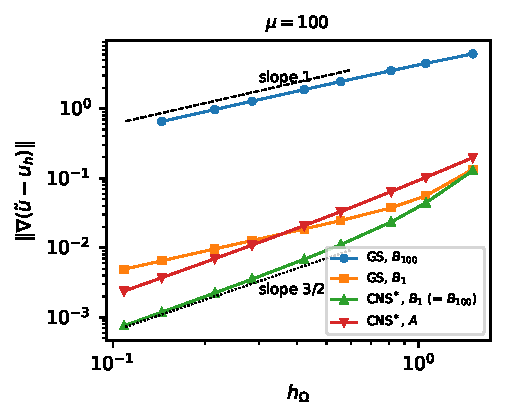
\includegraphics[width=0.48\textwidth]{figures/h1_rates.pdf}\hfill
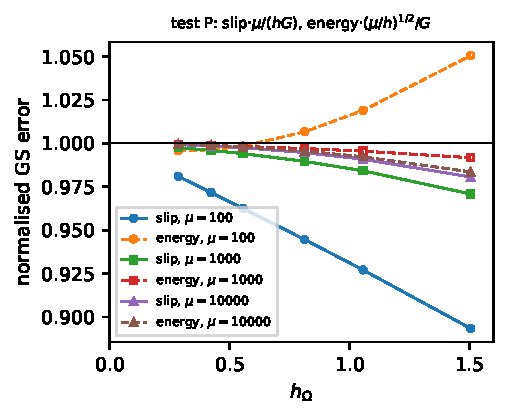
\includegraphics[width=0.48\textwidth]{figures/leading_term.pdf}
\caption{Left: $H^1$ errors at $\mu=100$. Once $G>0$, $\GS$ eventually has slope $1$, while $\CNS$ tends to slope $\frac32$ independently of the pressure. Right: the normalised slip and energy errors of $\GS$ on test P approach $1$ (Corollary~\ref{cor:Bp}).}
\label{fig:rates}
\end{figure}

\subsection{Pressure errors}
The pressure errors follow Section~\ref{sec:further} (Tables~\ref{tab:B100} and~\ref{tab:pB1}). For $\CNS$ the pressure error does not depend on the pressure data (for B$_1$, B$_{100}$ and C it agrees to $10^{-6}$ at $N=16$ and $3\cdot10^{-11}$ at $N=96$), and its $L^2$ rate decreases towards $\frac32$. For $\GS$ with $G>0$ the $L^2$ rate decreases towards $\frac12$; the first layer of triangles carries rate $0.48$--$0.50$ and the rest rate $0.9$--$1.0$, and the $L^\infty$ error on the first layer does not converge ($0.78$ for B$_1$, $77$ for B$_{100}$). On test P the first-layer pressure error of $\GS$ is $0.0958$ and $0.0793$ at $N=64$ and $96$, against $0.0961$ and $0.0796$ for the explicit first-layer field predicted by the theory. With $G=0$ (test A), $\GS$ behaves like $\CNS$.

\begin{table}[t]
\centering\small
\caption{$L^2$ pressure error $\norm{p^\circ-p_h}$, $\mu=100$. The ``off layer'' column is the $\GS$ error outside the first row of triangles, with the optimal constant removed.}\label{tab:pB1}
\begin{tabular}{rcccccc|cccc}
\toprule
 & \multicolumn{6}{c|}{test B$_1$ ($G>0$)} & \multicolumn{4}{c}{test A ($G=0$)}\\
$N$ & $\GS$ & rate & off layer & rate & $\CNS$ & rate & $\GS$ & rate & $\CNS$ & rate\\
\midrule
16 & $0.530$ & -- & $0.500$ & -- & $0.497$ & -- & $0.205$ & -- & $0.378$ & --\\
32 & $0.180$ & 1.22 & $0.121$ & 1.84 & $0.0767$ & 3.03 & $0.0648$ & 1.85 & $0.121$ & 1.81\\
48 & $0.137$ & 0.72 & $0.0805$ & 1.08 & $0.0287$ & 2.59 & $0.0329$ & 1.79 & $0.0623$ & 1.75\\
64 & $0.115$ & 0.61 & $0.0632$ & 0.88 & $0.0162$ & 2.08 & $0.0204$ & 1.73 & $0.0392$ & 1.69\\
96 & $0.0913$ & 0.60 & $0.0445$ & 0.89 & $0.00801$ & 1.80 & $0.0106$ & 1.68 & $0.0205$ & 1.65\\
\bottomrule
\end{tabular}
\end{table}

\subsection{The leak law and its constants}
Test P isolates the traction response exactly. Table~\ref{tab:P} and Figure~\ref{fig:rates} (right) show that the normalised slip and energy errors approach $1$, as Corollary~\ref{cor:Bp} predicts: at $N=96$ the energy ratios are within $0.5\%$ of $1$ for every $\mu$, and the defect of the slip ratio shrinks with $h/\mu$ ($0.019$, $0.0025$, $0.0007$ for $\mu=10^2,10^3,10^4$). Figure~\ref{fig:leak} shows the leak itself: at $N=32$, $\mu=100$, the normal trace of $u_h$ matches $(h/\mu)(p-\pbar)$ with relative $L^2(\Gh)$ misfit $0.055$, and the tangential trace is small and oscillates on the element scale. On test B$_1$ at $N=256$, $\GS$ itself gives slip and energy ratios $0.995$ and $1.001$.

The $H^1$ constant approaches the value $K=2.7565$ of Section~\ref{sec:leakflow} from both sides (Table~\ref{tab:hc}): from below at $\mu=100$, and from above at large $\mu$, where the excess is an element-scale oscillation nearly orthogonal to $U$ ($K_h^2\approx K^2(1+d_h^2)$; for example $2.7565\sqrt{1+0.175^2}=2.798$ against $2.796$ at $N=96$, $\mu=10^8$). The same slip and energy constants, and $H^1$ constants close to $K$, are observed for $k=5,6$ and on Clough--Tocher refinements with $k=2,3$ (Table~\ref{tab:Pv3}); for these elements the agreement with $K$ is observed, not proved.

\begin{table}[t]
\centering\small
\caption{The leading term of Corollary~\ref{cor:Bp}: normalised $\GS$ error on test P ($G=1.658$), $e=\ut-u_h$.}\label{tab:P}
\begin{tabular}{rrccc}
\toprule
$N$ & $\mu$ & $\norm{\nabla e}\,\mu/(hG)$ & $\norm{e}_{\Gh}\,\mu/(hG)$ & $\tnorm{e}(\mu/h)^{1/2}/G$\\
\midrule
16 & 100 & 2.464 & 0.893 & 1.050\\
32 & 100 & 2.612 & 0.945 & 1.007\\
64 & 100 & 2.684 & 0.972 & 0.996\\
96 & 100 & 2.708 & 0.981 & 0.996\\
96 & 1000 & 2.770 & 0.998 & 0.999\\
96 & 10000 & 2.790 & 0.9993 & 0.9994\\
\bottomrule
\end{tabular}
\end{table}

\begin{table}[t]
\centering\small
\caption{Approach to the $H^1$ constant $K=2.7565157$ (Theorem~\ref{thm:hc}) on test P: normalised $H^1$ error $K_h$ and relative $H^1$ distance $d_h$ between $(\mu/h)(\ut-u_h)$ and the leak flow, computed pointwise against the series solution.}\label{tab:hc}
\begin{tabular}{r|cc|cc|cc|cc}
\toprule
 & \multicolumn{2}{c|}{$\mu=10^2$} & \multicolumn{2}{c|}{$\mu=10^3$} & \multicolumn{2}{c|}{$\mu=10^4$} & \multicolumn{2}{c}{$\mu=10^8$}\\
$N$ & $K_h$ & $d_h$ & $K_h$ & $d_h$ & $K_h$ & $d_h$ & $K_h$ & $d_h$\\
\midrule
16 & 2.4642 & 0.193 & 2.7844 & 0.318 & 3.0562 & 0.539 & 3.3254 & 0.717\\
32 & 2.6117 & 0.124 & 2.7880 & 0.222 & 2.8751 & 0.323 & 2.9339 & 0.385\\
64 & 2.6843 & 0.084 & 2.7759 & 0.154 & 2.8082 & 0.206 & 2.8208 & 0.226\\
96 & 2.7084 & 0.067 & 2.7701 & 0.124 & 2.7899 & 0.163 & 2.7959 & 0.175\\
\bottomrule
\end{tabular}
\end{table}

\begin{figure}[t]
\centering
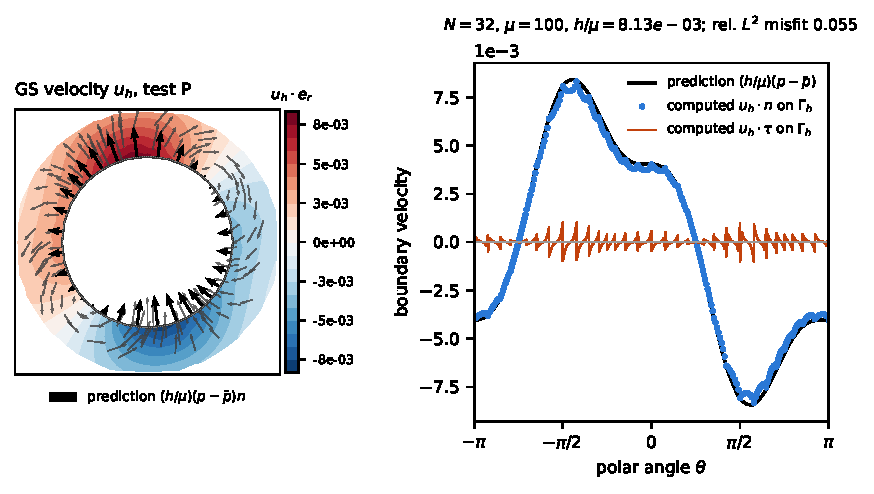
\includegraphics[width=\textwidth]{figures/leak_field.pdf}
\caption{The leak of the printed method on test P ($u=0$, so $u_h=-(\ut-u_h)$), $N=32$, $\mu=100$. Left: radial velocity $u_h\cdot e_r$ near the wall (colour) and $u_h$ (thin arrows); thick arrows show the prediction $(h/\mu)(p-\pbar)n$ at the chord midpoints. Right: normal and tangential traces of $u_h$ along $\Gh$ against $(h/\mu)(p-\pbar)$.}
\label{fig:leak}
\end{figure}

\begin{table}[t]
\centering\small
\caption{Normalised $\GS$ error on test P for other elements, at the finest level run.}\label{tab:Pv3}
\begin{tabular}{lrrccc}
\toprule
element & $\mu$ & $N$ & $\norm{\nabla e}\,\mu/(hG)$ & $\norm{e}_{\Gh}\,\mu/(hG)$ & $\tnorm{e}(\mu/h)^{1/2}/G$\\
\midrule
$k=5$ & 1000 & 128 & 2.768 & 0.9983 & 0.9994\\
$k=6$ & 1000 & 96 & 2.769 & 0.9976 & 0.9993\\
Clough--Tocher, $k=2$ & 1000 & 128 & 2.751 & 0.9982 & 0.9992\\
Clough--Tocher, $k=3$ & 1000 & 128 & 2.763 & 0.9983 & 0.9996\\
\bottomrule
\end{tabular}
\end{table}

\emph{Incompressibility is what saves the rate.} We computed exact discrete dual norms of the functionals used in the proofs, by saddle-point solves with the pointwise divergence constraint (Table~\ref{tab:lemma}). The dual norm of $v\mapsto\ip{S}{\dn v}$ with $S$ normal stays bounded on $\Zh$, but grows like $\hG^{-1/2}$ on $\VR$, and also on $\Zh$ for tangential $S$: exactly the dichotomy of Lemma~\ref{lem:cancel}. The transposed-gradient functional decays at rate $1.56$--$1.57$, confirming that the rate $\frac32$ of Lemma~\ref{lem:transposed} is sharp.

\begin{table}[t]
\centering\small
\caption{Exact discrete dual norms; rate in $\hG$ between $N=48$ and $N=64$ (positive means decay).}\label{tab:lemma}
\begin{tabular}{llc}
\toprule
functional & space & rate\\
\midrule
$\ip{S}{\dn v}$, $S$ normal & $\Zh$ & $+0.05$ (bounded, $\approx1.75$)\\
$\ip{S}{\dn v}$, $S$ normal & $\VR$ & $-0.52$\\
$\ip{S}{\dn v}$, $S$ tangential & $\Zh$ & $-0.52$\\
$\ip{(\nabla\ut)^{\mathsf T}n}{v}$, tests A / B & $\VR$ & $1.57$ / $1.56$\\
\bottomrule
\end{tabular}
\end{table}

\subsection{The penalty study}
The coercivity threshold $\mu^\ast$ on $\Zh$ is located by bisection on the inertia of the (unpivoted symmetric factorisation of the) velocity block augmented by a large multiple of the divergence penalty. Table~\ref{tab:thresh} and Figure~\ref{fig:thresh} give the results. Under refinement at fixed $h/\hG$, $\gamma^\ast$ increases by $3.4$, $1.8$ and $0.95$ per doubling, approaching the periodic-cell value $\gamma^\ast_\infty\approx21.4$ of Section~\ref{sec:penalty}. When the far field is coarsened with the wall fixed (part (b)), $\mu^\ast$ is linear in $h/\hG$ over more than a decade with slope $18$--$20$: the threshold is set locally at the wall, and the global normalisation of the penalty turns it into a $\rho$-scaling. For higher degree and on Clough--Tocher refinements the threshold is larger (Table~\ref{tab:threshv3}); in particular $\mu=100$ is \emph{below} the threshold for $k=5$ ($N\ge32$), $k=6$ and Clough--Tocher $k=3$, and our runs for those elements use $\mu=300$ and $1000$.

\begin{table}[t]
\centering\small
\caption{Coercivity threshold $\mu^\ast$ and $\gamma^\ast=\mu^\ast\hG/h$ ($k=4$).}\label{tab:thresh}
\textit{(a) Refinement at fixed $h/\hG\approx3.3$.}\\[2pt]
\begin{tabular}{lcccccccc}
\toprule
$N$ & 8 & 12 & 16 & 20 & 24 & 32 & 48 & 64\\
\midrule
$\rho$ & 3.41 & 4.16 & 4.70 & 5.08 & 5.36 & 5.73 & 6.13 & 6.35\\
$\mu^\ast$ & 50.3 & 51.8 & 59.3 & 60.3 & 63.3 & 66.0 & 69.1 & 70.7\\
$\gamma^\ast$ & 14.7 & 17.1 & 18.1 & 19.1 & 19.2 & 19.9 & 20.5 & 20.8\\
\bottomrule
\end{tabular}\par\vspace{6pt}
\textit{(b) Varying $h/\hG$ through the outer box $(-L,L)^2$.}\\[2pt]
\begin{tabular}{llccccc}
\toprule
 & $L$ & 2.5 & 5 & 10 & 20 & 40\\
\midrule
$N=16$ & $h/\hG$ & 3.28 & 5.90 & 11.3 & 22.2 & 43.9\\
 & $\mu^\ast$ & 59.3 & 112.1 & 208.0 & 411.5 & 809.3\\
\midrule
$N=32$ & $h/\hG$ & 3.33 & 5.79 & 10.8 & 21.1 & 41.5\\
 & $\mu^\ast$ & 66.0 & 113.9 & 218.0 & 422.2 & 835.7\\
\bottomrule
\end{tabular}
\end{table}

\begin{figure}[t]
\centering
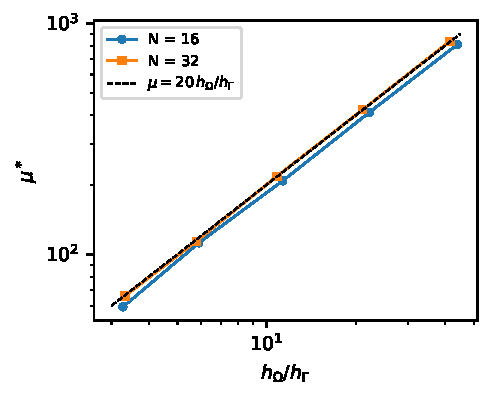
\includegraphics[width=0.55\textwidth]{figures/threshold.pdf}
\caption{Coercivity threshold $\mu^\ast$ against $h/\hG$ (Table~\ref{tab:thresh}(b)).}
\label{fig:thresh}
\end{figure}

\begin{table}[t]
\centering\small
\caption{Coercivity threshold $\gamma^\ast$ for higher degree and on Clough--Tocher (CT) refinements.}\label{tab:threshv3}
\begin{tabular}{lccccc}
\toprule
 & $N=8$ & $16$ & $32$ & $64$ & $128$\\
\midrule
$k=4$ & 14.7 & 18.1 & 19.9 & 20.8 & --\\
$k=5$ & 25.7 & 30.3 & 32.1 & 33.0 & --\\
$k=6$ & -- & 45.2 & 47.4 & 48.3 & --\\
CT, $k=2$ & 5.7 & 9.1 & 10.5 & 11.2 & 11.5\\
CT, $k=3$ & -- & 31.6 & 33.9 & 34.6 & --\\
\bottomrule
\end{tabular}
\end{table}

\emph{A growing penalty.} With $\mu=c(h_{16}/h)^\alpha$, $h_{16}=1.505$, the rates follow the predictions of Section~\ref{sec:growing} (Table~\ref{tab:rescue}). On test P, where only the leak is present, they are exactly $1+\alpha$ ($H^1$) and $(1+\alpha)/2$ (energy). On B$_1$ the $H^1$ rate of $\GS$ moves from $0.96$ to $1.42$--$1.52$ and the error at $N=96$ halves; on B$_1$ with $\alpha=\frac12$, $c=1000$ the measured energy rate $1.28$ is the geometric branch $(3-\alpha)/2$, the leak branch taking over only later.

\begin{table}[t]
\centering\small
\caption{$\GS$ (and $\CNS$) with $\mu=c(h_{16}/h)^\alpha$: rates between $N=64$ and $N=96$, and the asymptotic rates predicted in Section~\ref{sec:growing} (on test P, where only the leak is present, $1+\alpha$ and $(1+\alpha)/2$).}\label{tab:rescue}
\begin{tabular}{llccccc}
\toprule
test & method & $(\alpha,c)$ & $\norm{\nabla e}$ at $N=96$ & $H^1$ rate & energy rate & predicted\\
\midrule
P & $\GS$ & $(0,100)$ & $1.28\cdot10^{-2}$ & 0.95 & 0.49 & 1, 0.5\\
P & $\GS$ & $(\frac12,100)$ & $5.64\cdot10^{-3}$ & 1.45 & 0.73 & 1.5, 0.75\\
P & $\GS$ & $(1,100)$ & $2.47\cdot10^{-3}$ & 1.94 & 0.97 & 2, 1\\
B$_1$ & $\GS$ & $(0,100)$ & $1.27\cdot10^{-2}$ & 0.96 & 0.56 & 1, 0.5\\
B$_1$ & $\GS$ & $(\frac12,1000)$ & $5.81\cdot10^{-3}$ & 1.52 & 1.28 & 1.5, 0.75\\
B$_1$ & $\GS$ & $(1,100)$ & $5.03\cdot10^{-3}$ & 1.47 & 1.06 & 1.5, 1\\
B$_1$ & $\CNS$ & $(0,100)$ & $3.54\cdot10^{-3}$ & 1.64 & 1.53 & 1.5, 1.5\\
B$_1$ & $\CNS$ & $(1,100)$ & $5.21\cdot10^{-3}$ & 1.45 & 1.16 & 1.5, 1\\
A & $\GS$ & $(1,100)$ & $1.48\cdot10^{-2}$ & 1.34 & 1.16 & 1.5, 1\\
\bottomrule
\end{tabular}
\end{table} On test A ($G=0$) a growing penalty only costs: the $H^1$ constant moves towards that of the Dirichlet limit, $2.5$ times larger, and the energy error grows like $\gamma^{1/2}\hG^{3/2}$.

\emph{Flux correction.} Test F uses $\psi=(r^2-1)^3\sin(2x+1)\cos(\frac32y+\frac7{10})/400$ and $p=x^2y-y+x/2$: the cube makes $W\equiv0$, so the geometric slip $\norm{\ut}_{\Gh}$ is small, and the phase shifts break the symmetries, so the outer flux $m_R$ is nonzero (it decays like $h^{6.6}$). Every $z\in\Wh$ satisfies $\tnorm{\ut-z}\ge(\mu/h)^{1/2}|m_R|/|\Gh|^{1/2}$, a floor with constant exactly $1$. Table~\ref{tab:flux} shows the floor and its removal by the correction of Definition~\ref{def:flux}. Without correction the slip error of $\CNS$ is $(|m_R|^2/|\Gh|+\norm{\ut}^2_{\Gh})^{1/2}$ to three digits; with it, the slip error is $\norm{\ut}_{\Gh}$ to five digits. The $H^1$ errors with and without correction agree to relative $3\cdot10^{-6}$ ($N=16$) down to $10^{-9}$ ($N=64$), as Theorem~\ref{thm:unif} predicts.

\begin{table}[t]
\centering\small
\caption{Test F, $\CNS$ with uncorrected ($\gI$) and flux-corrected ($\tilde g_I$) outer data. Slip errors at $\mu=10^6$; energy errors at $\mu=10^8$, with the floor $(\mu/h)^{1/2}|m_R|/|\Gh|^{1/2}$.}\label{tab:flux}
\setlength{\tabcolsep}{3pt}
\begin{tabular}{rcccccccc}
\toprule
$N$ & $m_R$ & $\frac{|m_R|}{|\Gh|^{1/2}}$ & $\norm{\ut}_{\Gh}$ & slip, $\gI$ & slip, $\tilde g_I$ & $\tnorm e$, $\gI$ & $\tnorm e$, $\tilde g_I$ & floor\\
\midrule
16 & $2.04\cdot10^{-3}$ & $8.19\cdot10^{-4}$ & $2.40\cdot10^{-5}$ & $8.204\cdot10^{-4}$ & $2.396\cdot10^{-5}$ & 6.752 & 0.955 & 6.672\\
32 & $2.56\cdot10^{-5}$ & $1.02\cdot10^{-5}$ & $1.70\cdot10^{-6}$ & $1.038\cdot10^{-5}$ & $1.697\cdot10^{-6}$ & 0.187 & 0.149 & 0.114\\
64 & $3.75\cdot10^{-7}$ & $1.50\cdot10^{-7}$ & $1.09\cdot10^{-7}$ & $1.851\cdot10^{-7}$ & $1.091\cdot10^{-7}$ & 0.0123 & 0.0121 & 0.0023\\
\bottomrule
\end{tabular}
\end{table}

\emph{Higher degree and Clough--Tocher refinements.} Table~\ref{tab:ratesv3} gives $H^1$ rates at the finest pair of levels for $k=5,6$ and for Clough--Tocher refinements. $\CNS$ tends to rate $\frac32$ for $k=5,6$; $\GS$ tends to rate $1$ once $G>0$ (for $k=5$, $\mu=300$, its rate on B$_1$ decreases monotonically, $1.63,1.58,1.48,1.38,1.28,1.20$ for $N=24,\dots,128$), and the leak part $D:=u_{\GS}-u_{\CNS}$ already has rate $1.03$--$1.15$ and normalised slip and energy ratios within $1.5\%$ of $1$. At $\mu=1000$ the crossover of $\GS$ comes later, exactly as for $k=4$.

\begin{table}[t]
\centering\small
\caption{$H^1$ rates at the finest pair of levels (energy rate of $\CNS$ in parentheses); $D=u_{\GS}-u_{\CNS}$ is the leak part.}\label{tab:ratesv3}
\begin{tabular}{llrrccc}
\toprule
element & test & $\mu$ & $N$ & $\GS$ & $\CNS$ & $D$\\
\midrule
$k=5$ & B$_1$ & 300 & $96\to128$ & 1.20 & 1.59 (1.53) & 1.03\\
$k=5$ & B$_1$ & 1000 & $96\to128$ & 1.53 & 1.58 (1.54) & 1.13\\
$k=6$ & B$_1$ & 300 & $64\to96$ & 1.27 & 1.61 (1.54) & 1.04\\
$k=6$ & B$_1$ & 1000 & $64\to96$ & 1.57 & 1.61 (1.54) & 1.15\\
CT, $k=3$ & A & 1000 & $96\to128$ & 1.56 & 1.56 (1.55) & --\\
CT, $k=2$ & B$_1$ & 100 & $192\to256$ & 1.91 & 1.91 (1.91) & 1.01\\
\bottomrule
\end{tabular}
\end{table}

\subsection{Strong imposition and the \texorpdfstring{$h^{1/2}$}{h^(1/2)} phenomenon}\label{sec:num:strong}
Table~\ref{tab:strong} compares strongly imposed no-slip ($u_h=0$ at every node of $\Gh$, no Nitsche terms, same element) with $\GS$ and $\CNS$ on test A.
\begin{itemize}
\item On mesh (a) the first-layer diagonals alternate, so every other polygon vertex lies in only two triangles. The $H^1$ rate of strong imposition falls towards $\frac12$ ($0.56$ at $N=128$); the largest vertex-gradient error tends to $1.99$, which is $|\dn u\cdot\tau|=2$ for this flow: the discrete gradient vanishes at the locked vertices, and the pressure grows like $h^{-1/2}$ although $p\equiv0$. The counting lower bound of Theorem~\ref{thm:st:count} is within a factor $3.0$--$3.15$ of the measured error.
\item On mesh (s) every polygon vertex lies in three triangles, and strong imposition converges with rates $1.93\to1.61$, like the Nitsche methods, with an error about $2.5$ times larger. The slow drift of the rate (to $1.547$ at $N=192$) is a relative $O(\hG)$ correction: the data fit $E\approx a\hG^{3/2}(1+\beta\hG)$ with $\beta\approx1.1$--$1.3$. The vertex-gradient error decays like $h$, exactly as Lemma~\ref{lem:st:local}(d) predicts. Imposing $u_h=\ut$ instead of $0$ at the nodes of $\Gh$ gives rate about $4$: the whole defect is the transfer of the no-slip value from $\Gamma$ to $\Gh$.
\item $\GS$ and $\CNS$ do not see the change of mesh: at every $N\le128$ their errors on meshes (a) and (s) differ by at most $6\%$.
\item With a single locked vertex the strong-imposition rate falls to $1$ ($1.06$ at $N=128$), the raw pressure error does not converge, and the filtered pressure of Theorem~\ref{thm:st:locks}(d) converges at the velocity rate. With needles at the wall of angle $\varepsilon=0.3,\hG,\hG^2$ the rates approach $\frac32$, $1$, $\frac12$ as predicted, although the last two limits are not yet reached at $N\le96$.
\end{itemize}

\begin{table}[t]
\centering\small
\caption{Strong imposition against Nitsche: $H^1$ error, test A, $k=4$, $\mu=100$. Mesh (s): every polygon vertex in three triangles; mesh (a): alternating first-layer diagonals (vertices in two or four triangles).}\label{tab:strong}
\begin{tabular}{rrrrrrrrr}
\toprule
$N$ & \multicolumn{2}{c}{strong, (a)} & \multicolumn{2}{c}{strong, (s)} & \multicolumn{2}{c}{$\GS$, (s)} & \multicolumn{2}{c}{$\CNS$, (s)}\\
\cmidrule(lr){2-3} \cmidrule(lr){4-5} \cmidrule(lr){6-7} \cmidrule(lr){8-9}
 & error & rate & error & rate & error & rate & error & rate\\
\midrule
16 & $9.03\cdot10^{-1}$ & -- & $4.62\cdot10^{-1}$ & -- & $1.72\cdot10^{-1}$ & -- & $1.98\cdot10^{-1}$ & --\\
32 & $5.72\cdot10^{-1}$ & 0.72 & $1.43\cdot10^{-1}$ & 1.86 & $5.55\cdot10^{-2}$ & 1.79 & $6.41\cdot10^{-2}$ & 1.80\\
64 & $3.75\cdot10^{-1}$ & 0.62 & $4.56\cdot10^{-2}$ & 1.71 & $1.81\cdot10^{-2}$ & 1.68 & $2.08\cdot10^{-2}$ & 1.69\\
96 & $2.98\cdot10^{-1}$ & 0.59 & $2.38\cdot10^{-2}$ & 1.65 & $9.57\cdot10^{-3}$ & 1.63 & $1.09\cdot10^{-2}$ & 1.64\\
128 & $2.54\cdot10^{-1}$ & 0.56 & $1.52\cdot10^{-2}$ & 1.61 & $6.11\cdot10^{-3}$ & 1.59 & $6.96\cdot10^{-3}$ & 1.60\\
\bottomrule
\end{tabular}
\end{table}

\subsection{Caveats}
Three limitations should be kept in mind. First, the production penalty $\mu=100$ is close to the stability thresholds, as discussed above, so the measured constants are partly pre-asymptotic. Second, the manufactured solutions are smooth up to the corners of the box; for data-driven problems the corner singularities of the box would limit the bulk term (Assumption~\ref{ass:D}), though not the wall term that is the subject of this paper. Third, on Clough--Tocher refinements with $k=2,3$ the test pressure is not in the pressure space, and the pressure-independence of $\CNS$ holds only up to a term of order $h^{k+1/2}$ that scales with the amplitude of $p$; on test B$_1$ the rate $\frac32$ is not yet visible there, because the interpolation error of the steep velocity dominates \cite{PadhiExt}.

\section{Conclusions and open problems}\label{sec:conclusions}

Scott asked whether the Scott--Vogelius--Nitsche method on an inscribed polygon converges with error $\hG^{3/2}+\hO^k$ and, if not, why not. The answer has two halves. The first, announced in the joint letter \cite{CavalcantePadhiLetter} and proved in full here, concerns the method as printed: it converges, but with the expected error only when the pressure is constant along the wall, because without the pressure traction the penalty must balance the wall pressure and the discrete flow leaks through the wall at the rate $(h/\mu)(p-\pbar)$; restoring the traction with its wall mean removed, a device due to Frachon, Nilsson and Zahedi, gives a well-posed, exactly divergence-free method that attains $\hG^{3/2}+\hO^k$ for general data, and the term $\hG^{3/2}$ is sharp. The second half, which is the main new content of this paper, concerns the difficulty that motivated weak imposition in the first place. The zero-gradient lock is a property of the wall mesh: under the Guzm\'an--Scott angle condition strong imposition has the same two-sided rate $\hG^{3/2}+h^k$, and the lock comes from wall vertices in only two triangles, each costing $\hG|\dn u(z)|$, or from nearly singular wall stars. With Scott's normalisation the penalty must grow with the ratio of bulk to boundary mesh size, on every shape-regular mesh, but necessity cannot be read off a single wall star. Finally, the leak is explicit, with constant $1$ in the natural norms, and its $H^1$ size is the energy of a Stokes flow in the whole domain; incompressibility is what keeps the $H^1$ rate at $1$ rather than $\frac12$.

For practitioners the conclusions are simple. If exactly divergence-free velocities are to be combined with Nitsche's method on a polygonal approximation of a curved wall, the pressure traction must be included, with its wall mean removed, and the outer Dirichlet data should be corrected to zero net flux. The penalty should be scaled with the local chord length ($\gamma=\mu\hG/h\ge25$ is safe for $k=4$ on our meshes), and a mesh in which every wall vertex lies in at least three well-shaped triangles should be used, whatever the imposition. The attainable rate is $\hG^{3/2}$; higher rates require curved elements or boundary corrections \cite{NeilanOtus2021,DurstNeilan2024,LiuNeilanOtus2023,ChenLiu2026}.

Several questions remain open.
\begin{itemize}
\item \emph{Constants in the penalty analysis.} Necessity of $\mu\gtrsim\rho$ is proved on every shape-regular mesh, but with astronomically small constants; numerically $\mu^\ast\approx(15\text{--}16)\,h/\delta_1$, with $\delta_1$ the height of the first layer of triangles. An explicit, moderate constant for general meshes is open. The limit $\gamma^\ast_\infty\approx21.41$ of the threshold on our meshes is identified with a periodic cell value only modulo a discrete localisation inequality and a spline cut-off lemma that we have not proved.
\item \emph{The pressure of the corrected method.} Its lower bound needs a hypothesis on a boundary pressure moment; the cell problem that decides this hypothesis rests on a decay property verified only numerically and on a transplant lemma that is not proved. The sharpness of the rate $2$ for the drag of $\CNS$ at fixed penalty is open.
\item \emph{Other variants.} We have analysed the symmetric Nitsche form. The leak comes from the missing pressure term, not from the symmetry of the viscous terms, so we expect it in nonsymmetric variants as well, but we have not analysed these, nor penalty-free variants \cite{Burman2012,BoiveauBurman2016}, the slip-condition method of Gjerde and Scott \cite{GjerdeScott2022}, other divergence-free families, or cut meshes.
\item \emph{Strong imposition on general anisotropic meshes.} Our two-sided needle law assumes that every needle sits in its own pair at the wall; meshes whose needles do not come in isolated wall pairs are not covered.
\item \emph{Three dimensions.} The companion paper \cite{PadhiThreeD} treats inscribed polyhedra; the loss of the chordwise odd-symmetry cancellation changes several arguments there.
\end{itemize}
Finally, although Nitsche's method does not improve the rate on good meshes, it is robust on bad ones: the Nitsche methods were insensitive to locked wall vertices in all our computations. Proving this robustness, on meshes that violate (M2) at the wall, is perhaps the most natural next question.

\section*{Declarations}

\subsection*{Use of generative AI}
The research reported here was carried out by the author with extensive use of a generative AI model, Claude (Anthropic; model Claude Opus~5.5), and we describe that use in detail.
\begin{itemize}
\item \emph{Mathematics.} The model was used to develop proof strategies and to draft and check proofs of the lemmas and theorems, including the leak analysis, the lower bounds, the penalty witnesses and the strong-imposition theory.
\item \emph{Code.} The model wrote and ran the finite element code (the Scott--Vogelius--Nitsche solver, the penalty-threshold and dual-norm computations), the exact rational-arithmetic and interval certificates, and the scripts that produce the tables and figures.
\item \emph{Literature.} The model was used for literature search and for checking bibliographic data and the content of cited results.
\item \emph{Writing.} The model drafted and edited the text of this article and of its extended version.
\end{itemize}
We did not treat the model's output as verified. The proofs were subjected to independent checks by separate AI instances (fresh sessions of the model instructed to act as critical referees of individual arguments), and every error found in this way was corrected or the corresponding claim weakened; the author reviewed these referee reports and the resulting corrections, which are recorded in the public repository. Claims that could not be fully proved are labelled as numerical, conditional or open, here and in \cite{PadhiExt}. The computer-assisted steps (the penalty certificates and the star-condition constants) use exact rational or rigorous interval arithmetic, with negative controls. All numbers in the tables were checked against the logs of reproducible runs, and the code, raw outputs and logs are public \cite{ZeroGradRepo}. The author directed the project, made the decisions on what to prove and how to present it, and takes full responsibility for the content of this article, including any remaining errors. The AI model is not an author.

\subsection*{Data and code availability}
All code, raw results and logs, and the scripts that regenerate every table and figure, are available at \url{https://github.com/jaideepsaipadhi/zero-gradient-prize} \cite{ZeroGradRepo}. The extended version of this article, with all omitted proofs and computations, is archived on Zenodo \cite{PadhiExt}.

\subsection*{Competing interests}
The question studied in this article is the subject of a prize offered by L.~R.~Scott (Prize Problem Ledger problem PPL~115 \cite{ScottPrize}), and the author intends to submit this work for it. The author declares no other competing interests.
%% TBD: if the joint AML letter with C. de S. Cavalcante is submitted, disclose it here (and cite it in Section 2).

\subsection*{Funding}
This research received no external funding.
%% VERIFY with the author.

\subsection*{Acknowledgements}
The author thanks L.~Ridgway Scott for posing the problem and for making the prize statement and the computations of \cite{GjerdeScott2024} publicly available.
%% TBD: further acknowledgements (e.g. correspondence with Scott and Cavalcante), at the author's discretion.


\bibliographystyle{amsplain}
\bibliography{refs}

\end{document}
